\documentclass[11pt]{article}
\ifdefined\pdfinfoomitdate\pdfinfoomitdate=1\fi
\ifdefined\pdftrailerid\pdftrailerid{}\fi
\ifdefined\pdfsuppressptexinfo\pdfsuppressptexinfo=15\fi
\usepackage[T1]{fontenc}
\usepackage{lmodern}
\usepackage[margin=1in]{geometry}
\usepackage{amsmath,amssymb,amsthm,mathtools}
\usepackage{microtype}
\usepackage{enumitem,booktabs}
\usepackage{xcolor,tikz}
\usetikzlibrary{arrows.meta,positioning,calc,patterns,decorations.pathreplacing}
\usepackage[numbers,sort&compress]{natbib}
\usepackage[hyphens]{url}
\usepackage{hyperref}
\hypersetup{colorlinks=true,linkcolor=blue!45!black,citecolor=blue!45!black,
 urlcolor=blue!45!black,pdfauthor={OpenAI},
 pdftitle={Equidistribution of Primitive Sextic Torus Packets}}
\numberwithin{equation}{section}
\newtheorem{theorem}{Theorem}[section]
\newtheorem{lemma}[theorem]{Lemma}
\newtheorem{proposition}[theorem]{Proposition}
\newtheorem{corollary}[theorem]{Corollary}
\theoremstyle{definition}
\newtheorem{definition}[theorem]{Definition}
\theoremstyle{remark}
\newtheorem{remark}[theorem]{Remark}
\newcommand{\R}{\mathbb R}
\newcommand{\Z}{\mathbb Z}
\newcommand{\N}{\mathbb N}
\newcommand{\Q}{\mathbb Q}
\newcommand{\C}{\mathbb C}
\newcommand{\E}{\mathbb E}
\newcommand{\Prb}{\mathbb P}
\newcommand{\one}{\mathbf 1}
\newcommand{\dd}{\mathop{}\!d}
\newcommand{\idtext}[1]{\begingroup\urlstyle{same}\nolinkurl{#1}\endgroup}
\DeclareMathOperator{\supp}{supp}
\DeclareMathOperator{\SL}{SL}
\DeclareMathOperator{\GL}{GL}
\DeclareMathOperator{\Ad}{Ad}
\DeclareMathOperator{\diag}{diag}
\DeclareMathOperator{\Tr}{Tr}
\DeclareMathOperator{\covol}{covol}
\DeclareMathOperator{\Disc}{Disc}
\DeclareMathOperator{\vol}{vol}
\DeclareMathOperator{\Res}{Res}
\DeclareMathOperator{\Fix}{Fix}
\DeclareMathOperator{\Mat}{Mat}
\DeclareMathOperator{\End}{End}
\DeclareMathOperator{\Var}{Var}
\DeclareMathOperator{\dist}{dist}
\DeclareMathOperator{\diam}{diam}
\DeclareMathOperator{\sgn}{sgn}
\DeclareMathOperator{\rank}{rank}
\setlist[enumerate]{leftmargin=*,itemsep=4pt}
\setlength{\emergencystretch}{2em}
\setcounter{tocdepth}{1}
\title{Equidistribution of Primitive Sextic Torus Packets}
\author{OpenAI}
\date{October 5, 2026}
\begin{document}
\maketitle
\begin{abstract}
We prove that the complete ideal-class packets of maximal orders in
totally real sextic fields with no proper intermediate fields become
equidistributed, with no escape of mass, in the space of unimodular
lattices as their field discriminants tend to infinity. The limit is
Haar probability measure. Each packet includes all coordinate-sign
translates and is weighted by diagonal-orbit volume.
\end{abstract}
\tableofcontents
\section{Introduction}\label{sec:introduction}

The real embeddings of a totally real number field turn its ideals into
lattices. Multiplication by positive diagonal matrices changes the relative
sizes of the embedding coordinates while preserving covolume. The units
make each resulting diagonal orbit compact, and the ideal classes assemble
these orbits into a finite packet. The distribution of such packets connects
the arithmetic of number fields with the dynamics of higher-rank diagonal
groups. We prove equidistribution for totally real sextic fields having no
proper intermediate field.

\subsection{Packets and the main theorem}

Let
\[
 X_6=\SL_6(\Z)\backslash\SL_6(\R),\qquad
 A_6=\{\diag(e^{u_1},\ldots,e^{u_6}):\textstyle\sum_j u_j=0\}.
\]
We regard $X_6$ as the space of covolume-one lattices in $\R^6$, with
matrices acting on row vectors on the right. Let $m_6$ denote its
$\SL_6(\R)$-invariant probability. We normalize Haar measure on $A_6$
as $\dd u_1\cdots\dd u_5$, with $u_6=-\sum_{j=1}^5u_j$.

A degree-six number field $K$ is \emph{primitive} if there is no field
$F$ with $\Q\subsetneq F\subsetneq K$. Suppose $K$ is totally real,
choose an ordering $\sigma=(\sigma_1,\ldots,\sigma_6)$ of its real
embeddings, and write $\mathcal O_K$ for its ring of integers. For a
nonzero fractional $\mathcal O_K$-ideal $I$, set
\[
 \sigma(I)=\{(\sigma_1(d),\ldots,\sigma_6(d)):d\in I\},\qquad
 \Lambda_{I,\sigma}=\covol(\sigma(I))^{-1/6}\sigma(I).
\]
Choose one representative of each ordinary ideal class. Let
$\mathcal P_{K,\sigma}$ be the set of distinct compact orbits
\[
 \Lambda_{I,\sigma}wA_6,
 \qquad w=\diag(\epsilon_1,\ldots,\epsilon_6),\quad
 \epsilon_j\in\{1,-1\}.
\]
Here every sign matrix acts on the underlying lattice, including those
of determinant $-1$. Dirichlet's unit theorem gives compactness of the
orbits. Including all signs makes the packet independent of the chosen
ordinary ideal-class representatives.

For $\mathcal O\in\mathcal P_{K,\sigma}$, let $m_{\mathcal O}$ be
its invariant probability and $\vol_A(\mathcal O)$ its volume for the
specified Haar measure. The packet probability is
\begin{equation}\label{eq:packet-definition}
 \mu_{K,\sigma}=
 \frac{\displaystyle\sum_{\mathcal O\in\mathcal P_{K,\sigma}}
              \vol_A(\mathcal O)m_{\mathcal O}}
      {\displaystyle\sum_{\mathcal O\in\mathcal P_{K,\sigma}}
              \vol_A(\mathcal O)}.
\end{equation}

\begin{theorem}\label{thm:main}
Let $K_i$ be totally real primitive fields of degree six, with
$|\Disc(K_i)|\to\infty$, and choose any ordering $\sigma_i$ of the
embeddings of each field. Then
\[
 \int_{X_6} f\,\dd\mu_{K_i,\sigma_i}
       \longrightarrow\int_{X_6} f\,\dd m_6
       \qquad(f\in C_c(X_6)).
\]
There is no escape of mass: for every $\epsilon>0$ there is a compact
$C\subset X_6$ such that
$\mu_{K_i,\sigma_i}(C)\ge1-\epsilon$ for all sufficiently large $i$.
\end{theorem}

The theorem concerns each complete packet attached to a field. It allows
the fields and their embedding orderings to vary freely under the stated
hypotheses. The arithmetic role of primitivity is to make every
nonrational integer of $K_i$ generate the full field; this will yield
uniform separation in the dual lattice used to count thin tubes.

\subsection{History and the composite-degree obstruction}

For real quadratic fields, the corresponding packets project to packets
of closed geodesics on the modular surface. Linnik's ergodic method,
including Skubenko's treatment of the one-sheeted hyperboloid, gave
equidistribution under an auxiliary splitting condition
\cite[Chapter~VI]{Linnik1968}; see also the historical statements in
\cite[Theorems~1.1--1.2]{ELMV2012}. Duke removed this condition for
fundamental discriminants by analytic methods
\cite[Theorem~1]{Duke1988}. Einsiedler, Lindenstrauss, Michel, and
Venkatesh later gave a dynamical proof formulated for all positive
nonsquare order discriminants~\cite[Theorem~2.3]{ELMV2012}.
In higher degree the compact diagonal orbits have dimension greater
than one, and the dynamics of the full diagonal group provides
additional rigidity.

Einsiedler, Katok, and Lindenstrauss proved that, on
$\SL_d(\Z)\backslash\SL_d(\R)$ for $d\ge3$, an ergodic probability
invariant under the full positive diagonal group and having positive
entropy for a diagonal flow is algebraic~\cite[Theorem~1.3]{EKL2006}.
Einsiedler, Lindenstrauss, Michel,
and Venkatesh developed the connection between arithmetic separation of
periodic torus orbits and entropy of their limiting measures
\cite{ELMV2009}. Their subsequent cubic equidistribution theorem
combined measure classification, subconvexity, and local harmonic
analysis~\cite{ELMV2011}. These works distinguish two tasks that remain
central here: establishing nonescape and entropy, and identifying the
algebraic components of a limit.

The second task is particularly important in composite degree
\cite[Section~1.6.3]{ELMV2011}. In prime
degree, the positive-entropy classification gives Haar measure directly
\cite[Corollary~1.4]{EKL2006}. In degree six there are proper block
subgroups containing the full diagonal group whose closed orbits can
carry finite invariant measures. Primitivity of the fields in the
sequence does not, by itself, rule out concentration near such orbits.
The proof must retain enough information from the sequence to exclude
these limiting components.

Subsequent work has sharpened the entropy estimates in higher degree.
Khayutin obtained bounds for maximal-order packets whose Galois closures
act two-transitively on the embeddings~\cite[Theorem~1.1]{Khayutin2019}.
Wieser and Yang obtained entropy bounds for quartic packets of maximal
type with quadratic subfields, under a fixed split-place condition and
additional discriminant-growth hypotheses~\cite{WieserYang2026}.
These results clarify the arithmetic information available in composite
degree; identifying every component of a limit remains a separate step
in the argument here.

The arithmetic preparation adapts the ordinary-vector method used for
prime-degree packets~\cite[Sections~2--6]{PrimeDegreePackets} and primitive
quartic packets~\cite[Section~3]{QuarticPackets}. We give the needed estimates in full.
They use Stark's effective zero-free information
\cite{Stark1974} and the short-interval bounds of Shiu and Pollack
\cite{Shiu1980,Pollack2020}. The quartic work treats its additional
obstruction using exterior-square arithmetic. Here an ordinary vector
and a dual vector produce a codifferent element, and primitivity gives
the separation needed to estimate its partial traces.

\subsection{The intermediate-resolution argument}

The main additional argument concerns conditional measures that retain
information at growing, but separated, resolutions. We describe its
purpose before introducing the construction.

Let $\mu_i=\mu_{K_i,\sigma_i}$. Ordinary-vector estimates prove
tightness and give every probability limit $\mu$ an $O(r^6)$ bound
for the mass of radius-$r$ balls, uniformly when their centers range
over a compact set. Since $A_6$ has dimension five, this bound
forces positive entropy in almost every $A_6$-ergodic component.
Theorem~\ref{thm:ekl} then makes those components homogeneous.
Every proper component is supported on points fixed by a nonidentity
diagonal matrix with algebraic entries, so only a countable family of
fixed-point sets must be excluded.

The arithmetic estimate used for this exclusion concerns two-sided
tubes, with $O$ a sufficiently small identity neighborhood,
\[
 x\bigl(a(tb)Oa(-tb)\cap a(-tb)Oa(tb)\bigr),
 \qquad a(b)=\diag(e^{b_1},\ldots,e^{b_6}),\quad\sum_jb_j=0.
\]
If the coordinates of $b$ are separated across a prescribed cut of the
indices, ordinary and dual vectors bound the packet mass of such a
tube by $e^{-\eta t}$ for a fixed $\eta>0$. The estimate holds throughout a growing interval
$[T_{-,i},T_{+,i}]$ with $T_{+,i}/T_{-,i}\to\infty$.
The breadth of this interval is used throughout the proof.

For $j\ne k$, let $U_{jk}=\{1+sE_{jk}:s\in\R\}$.
Exact conditional measures of a finite packet along these root groups
are supported at a single point. They therefore cannot express the
spread detected by the arithmetic tube bound. Instead, in a local box
$(q,h)$ for a unipotent group, we condition the plaque coordinate $h$
on a small cell of the transverse coordinate $q$. We choose logarithmic
cell depths inside the growing interval so that the conditional
probabilities change negligibly across a much wider internal range.
In their joint limits with the sampled lattice, the plaque point still
has the recorded probability as its conditional law, given the transverse
coordinate and that one probability. This sampling identity will detect
atoms on sets meeting each root plaque in only countably many points.
The limiting probabilities also retain their behavior under suitable
long diagonal motions.

Product structure for genuine leafwise measures and the use of
noncommuting root foliations are basic ingredients of the higher-rank
entropy method of Einsiedler and Katok
\cite[Proposition~8.3]{EK2003}~\cite[Theorems~8.4--8.5]{EK2005};
see also~\cite[Corollary~8.8 and Theorem~9.8]{EL2010}. The point here is
to prove the corresponding structure for the conditional probabilities
formed before taking the limit. If a diagonal element fixes one root
group $U$ and contracts a complementary unipotent subgroup $W$ generated
by root groups and normal in $WU$,
the limiting measure on $WU$ is the product of the limiting measures
on $W$ and $U$. Contraction identifies the $U$ factor. A separate
conditional-information argument shows that adding a fine $U$-cell label
barely changes the law of any fixed further subdivision of a typical
$W$ tile. Expanding that tile turns this comparison into one for bounded
$W$ tests and identifies the $W$ factor. Both arguments are needed, and neither
follows by simply disintegrating the weak limit.

Call $j\to k$ active when the resulting $U_{jk}$ measure has support
beyond the identity. The product rule makes activity transitive under
composition of roots. It also permits an entropy argument: if crossing
roots are inactive along a positive proportion of long trajectories,
then their names can be encoded using only the slowly expanding
directions inside the two sides of a cut. This contradicts the tube
bound. Long motions in the diagonal wall $b_j=b_k$ fixing $U_{jk}$ leave
its activity unchanged. Combining the resulting one-dimensional functions
of the differences $b_k-b_j$ upgrades activity along trajectories to full
activity at almost every limiting state. A proper homogeneous
fixed-point piece forces an inactive root and is therefore excluded.

The construction separates the arithmetic estimate from this last
argument. Its potentially reusable ingredients are the comparison of
conditional probabilities across a broad range of transverse depths,
their product rule, and the passage from entropy bounds for long segments
starting in any fixed positive proportion of a packet to full root activity.

Section~\ref{sec:arithmetic} proves the arithmetic bounds, and
Section~\ref{sec:homogeneous} identifies the homogeneous alternatives.
Sections~\ref{sec:conditioning} and~\ref{sec:product} construct and
factor the intermediate conditional measures.
Section~\ref{sec:activity} records their root-group consequences.
Sections~\ref{sec:segment-entropy} and~\ref{sec:combination} prove the
long-segment and full-activity assertions, respectively, and
Section~\ref{sec:assembly} concludes the proof.

\subsection{Conventions}

For the remainder of the paper write $n=6$,
$G=\SL_n(\R)$, $\Gamma=\SL_n(\Z)$, $X=\Gamma\backslash G$,
and $A=A_n$. Let $L=\{b\in\R^n:\sum_j b_j=0\}$, identified with the
traceless diagonal matrices, and
$a(b)=\diag(e^{b_1},\ldots,e^{b_n})$. We use the right action
throughout. Thus motion by $a(b)$ changes a relative displacement $h$
to $a(-b)ha(b)$.
Matrix neighborhoods of the identity and smooth metrics are interchangeable
on fixed compact sets. When a metric on all of $X$ is needed, we use
the quotient of a left-invariant Riemannian metric on $G$.
The notation $B(r)$ denotes a sufficiently small identity neighborhood
of radius $r$. Implicit constants may depend on fixed compact sets,
charts, and $n$, but not on the varying field. All passages to
subsequences preserve the probability limit under consideration.

\section{Arithmetic estimates for the packets}\label{sec:arithmetic}

This section establishes the three estimates on which the dynamical
argument rests: uniform control of the cusp, a dimension bound for
probability limits, and exponential decay on two-sided diagonal tubes.
The first two follow by counting ordinary lattice vectors.  For the
third, we count an ordinary vector together with a dual vector; their
coordinatewise product lies in the codifferent and can be counted in a
thin slice.

For the volume, unfolding, and ordinary-vector estimates, we adapt
the method of \cite[Sections~2--6]{PrimeDegreePackets} and
\cite[Section~3]{QuarticPackets}.  We reproduce the needed arguments
in the packet and Haar normalizations of this paper.

Throughout this section, $K$ is a totally real field of degree six with
no proper intermediate field, and $\sigma$ is an ordering of its real
embeddings.  Write
\[
 D=|\Disc(K)|,\qquad Q=D^{1/2},\qquad
 \kappa=\mathop{\rm Res}_{s=1}\zeta_K(s),\qquad
 d_K(l)=\#\{\mathfrak b\subset\mathcal O_K:N\mathfrak b=l\}.
\]
All ideals counted here are nonzero.  For a sequence of fields and
embedding orderings, we use the corresponding notation
\[
 D_i=|\Disc(K_i)|,\qquad Q_i=D_i^{1/2},\qquad
 \kappa_i=\mathop{\rm Res}_{s=1}\zeta_{K_i}(s),\qquad
 \mu_i=\mu_{K_i,\sigma_i}.
\]
Unless another dependence is indicated, constants below are absolute
for this fixed degree.  In particular, they are independent of the
field and of the ordering of its embeddings.

\subsection{Volume and unfolding}

We first make the sign convention in the packet definition explicit.
The space $X=\SL_6(\Z)\backslash\SL_6(\R)$ parametrizes ordinary
unimodular lattices: a lattice has a positively oriented basis, and
any two such bases differ by an element of $\SL_6(\Z)$.  Consequently
a diagonal sign matrix acts on lattices even when its determinant is
$-1$.  The resulting lattice again represents a point of $X$ by choosing
a positively oriented basis.  There is no additional orientation
coordinate.

Let $h_K$ and $R_K$ denote the ordinary class number and regulator,
respectively.  Our convention for $R_K$ is the covolume of the absolute
logarithms of the units after deleting the sixth coordinate.  Put
\[
 U=\mathcal O_K^\times,\qquad
 U^+=\{\epsilon\in U:\sigma_j(\epsilon)>0\ (1\le j\le6)\},
 \qquad s=[U:U^+].
\]
For a nonnegative Borel function $f$ on $\R^6$, define its lattice sum by
\[
 \widehat f(\Lambda)=\sum_{v\in\Lambda\setminus\{0\}}f(v).
\]
For $p>0$, define a logarithmic fiber integral
\begin{align}
 V_f(p)
  =\sum_{\epsilon\in\{\pm1\}^6}\int_{\R^5}
  f\bigl(\epsilon_1e^{u_1},\ldots,\epsilon_5e^{u_5},
     \epsilon_6p e^{-u_1-\cdots-u_5}\bigr)
       \,\dd u_1\cdots\dd u_5 .                 \label{eq:fiber-integral}
\end{align}
Thus $V_f(p)$ integrates over the set on which the absolute product of
the six coordinates is $p$, with the Haar normalization used for $A$.

\begin{proposition}[Packet volume and vector unfolding]
\label{prop:packet-volume}
Every orbit in $\mathcal P_{K,\sigma}$ has $A$-volume $(s/2)R_K$,
and there are $h_K2^6/s$ distinct orbits.  In particular, the total
packet volume is $Q\kappa$.  For every nonnegative Borel function $f$,
\begin{equation}
 \int_X\widehat f\,\dd\mu_{K,\sigma}
   =\frac1{Q\kappa}\sum_{l\ge1}d_K(l)V_f(l/Q),
                                                        \label{eq:vector-unfolding}
\end{equation}
where both sides are allowed to be infinite.
\end{proposition}

\begin{proof}
The only roots of unity in a totally real field are $1$ and $-1$.
The kernel of the absolute logarithmic map on $U$ therefore has
order two.  Its image on $U^+$ has index $s/2$ in its image on $U$.
The unit theorem now gives covolume $(s/2)R_K$ for the positive-unit
logarithms in the coordinates $u_1,\ldots,u_5$.

We check that these are exactly the stabilizers and identifications
in the packet.  Suppose a real diagonal map sends $\sigma(I)$ onto
$\sigma(J)$.  Choose $0\ne d\in I$, and let its image be $\sigma(e)$
with $e\in J$.  All embeddings of $d$ are nonzero, so the diagonal
entries of the map are $\sigma_j(e/d)$.  It is multiplication by
$e/d\in K^\times$, and hence $J=(e/d)I$.  This observation also
applies to normalized lattices after their positive covolume factors
have been undone.  It follows that different ordinary ideal classes
give disjoint packet orbits.  For a fixed ideal, the diagonal
automorphisms are its units, because $(I:I)=\mathcal O_K$.

The stabilizer in $A$ is consequently the image of $U^+$.
Two sign translates belong to the same $A$-orbit exactly when their
signs differ by a unit signature.  The signature image has cardinality
$s$, giving $2^6/s$ orbits for each ordinary class and the stated orbit
volume.  The analytic class number formula, in this normalization, is
\[
 Q\kappa=2^5h_KR_K.
\]
It agrees with the product of the orbit number and orbit volume.

For completeness, let $\mathcal F$ be a fundamental domain for the
positive-unit logarithms in the traceless diagonal algebra.  Summing
over ordinary ideal-class representatives and all sign matrices
counts each orbit exactly $s$ times.  Thus for any nonnegative $F$ on
$X$,
\begin{equation}
 \int_XF\,\dd\mu_{K,\sigma}
 =\frac1{sQ\kappa}\sum_{[I]}\sum_w
   \int_{\mathcal F}F(\Lambda_{I,\sigma}w a(u))\,\dd u.
                                                        \label{eq:packet-integral}
\end{equation}
Here $\dd u=\dd u_1\cdots\dd u_5$ and the sixth coordinate is minus
their sum.

Apply this identity to $F=\widehat f$.  A nonzero $d\in I$ determines
the integral ideal
\[
 \mathfrak b=(d)I^{-1},
 \qquad
 \prod_{j=1}^6
 \left|\covol(\sigma(I))^{-1/6}\sigma_j(d)\right|
 =\frac{N\mathfrak b}{Q},
\]
because $\covol(\sigma(I))=QNI$.  The ideal $\mathfrak b$
determines the class $[I]=[\mathfrak b]^{-1}$, and every integral
$\mathfrak b$ occurs.  For that ideal, the possible $d$ form a single
$U$-orbit, or $s$ orbits under $U^+$.  Summing a positive-unit orbit
and integrating over $\mathcal F$ unfolds to the entire traceless
diagonal algebra.  Multiplication by a representative of $U/U^+$
translates the absolute logarithms and permutes the signs.  After the
sum over $w$, each of these $s$ orbits therefore contributes
$V_f(N\mathfrak b/Q)$.  Their number cancels the factor $s$ in
\eqref{eq:packet-integral}, proving \eqref{eq:vector-unfolding}.
All rearrangements are justified by nonnegativity.
\end{proof}

\subsection{Uniform counts of ideals}

The normalization by $\kappa$ in \eqref{eq:vector-unfolding} makes it
important to keep this same factor in upper bounds for ideal counts.
We obtain it from a zero-free neighborhood of $1$, followed by Shiu's
estimate for nonnegative multiplicative functions.

\begin{lemma}[Uniform ideal estimates]\label{lem:ideal-estimate}
For all sufficiently large discriminants $D$ in the present family,
\begin{align}
 \kappa&\gg (\log D)^{-1},                         \label{eq:residue-lower}\\
 \sum_{p\le D}\frac{d_K(p)}p
   &\le \log(\kappa\log D)+O(1),                 \label{eq:prime-sum}\\
 \sum_{x-y<l\le x}d_K(l)&\ll y\kappa
 \quad\left(D^{1/4}\le x\le D,
                    \ x^{1/2}\le y\le x\right).  \label{eq:ideal-interval}
\end{align}
In \eqref{eq:prime-sum}, $p$ ranges over rational primes.  The constants
and the discriminant threshold are uniform in $K$.
\end{lemma}

\begin{proof}
We first record the precise zero exclusion needed here.  Stark's
Lemma~3 shows that the rectangle
\[
 \Re s\ge1-\frac1{4\log D},\qquad
 |\Im s|\le\frac1{4\log D}
\]
contains at most one nontrivial zero of $\zeta_K$, and that such a
zero is real and simple.  His Lemma~8 applies also to nonnormal
fields: a real zero $\beta$ with
\[
 1-\frac1{4\cdot6!\log D}\le\beta<1
\]
would be a zero of the zeta function of a quadratic subfield of $K$
\cite[Lemmas~3 and~8]{Stark1974}.  Our field has no such subfield.
Consequently, for an absolute $c_0>0$,
\begin{equation}
 |1-\rho|\ge \frac{c_0}{\log D}
 \quad\text{for every nontrivial zero $\rho$ of $\zeta_K$}.
                                                        \label{eq:zero-exclusion}
\end{equation}
One can take $c_0=1/2880$.  This use of Stark's result does not require
$K/\Q$ to be normal.

Set $s_0=1+1/\log D$.  The logarithmic derivative of the completed
Dedekind zeta function gives, for real $1<s\le s_0$,
\begin{equation}
 S(s):=\sum_\rho\Re\frac1{s-\rho}
   =\frac1{s-1}+\frac12\log D
        +\frac{\zeta'_K(s)}{\zeta_K(s)}+O(1).
                                                        \label{eq:zeta-derivative}
\end{equation}
The zeros are counted with multiplicity.  The real-part sum converges,
and the gamma-factor contribution is bounded uniformly because the
degree and signature are fixed.  Each summand on the left is
nonnegative, and $\zeta'_K(s_0)/\zeta_K(s_0)\le0$ by its Dirichlet
series.  Hence $S(s_0)\ll\log D$.

The same estimate holds throughout $(1,s_0]$.  Indeed, writing
$a=1-\Re\rho\ge0$, $v=\Im\rho$, and $u=s-1$, the relevant term is
\[
 \frac{a+u}{(a+u)^2+v^2}.
\]
For $0<u\le1/\log D$, its numerator does not exceed its numerator
at $s_0$, while \eqref{eq:zero-exclusion} gives
$a^2+v^2\ge c_0^2/(\log D)^2$.  The denominator at $s_0$ is
therefore at most a constant multiple of the denominator at $s$.
Termwise comparison proves the asserted uniform estimate for $S(s)$.
Integrating \eqref{eq:zeta-derivative} after moving $1/(s-1)$ to the
other side now gives
\begin{equation}
 \zeta_K(s_0)\asymp\kappa\log D.                 \label{eq:zeta-residue-comparison}
\end{equation}
More explicitly, the logarithmic derivative of
$(s-1)\zeta_K(s)$ is $S(s)-\tfrac12\log D+O(1)$, whose integral
over this interval is $O(1)$, and its limit at $s=1$ is $\kappa$.
Since $\zeta_K(s_0)\ge1$, this proves \eqref{eq:residue-lower}.

The Euler product gives
\[
 \sum_{p\le D}\frac{d_K(p)}{p^{s_0}}
      \le\log\zeta_K(s_0).
\]
Also $d_K(p)\le6$ and
\[
 \sum_{p\le D}d_K(p)\left(\frac1p-\frac1{p^{s_0}}\right)
 \le\frac6{\log D}\sum_{p\le D}\frac{\log p}{p}\ll1,
\]
where the final estimate follows from Chebyshev's bound by partial
summation.  Equation~\eqref{eq:zeta-residue-comparison} now proves
\eqref{eq:prime-sum}.

To obtain the interval estimate, we use Shiu's theorem
\cite{Shiu1980}, in the formulation of
\cite[Theorem~1.1]{Pollack2020} with empty excluded residue sets.
For a nonnegative multiplicative function $f$, the hypotheses are
\[
 f(p^a)\le A_1^a,
 \qquad
 f(m)\le A_2(\epsilon)m^\epsilon
       \quad(\epsilon>0).
\]
For any fixed $0<\beta<1/2$, the conclusion is
\begin{equation}
 \sum_{x-y<m\le x}f(m)
 \ll\frac y{\log x}
     \exp\left(\sum_{p\le x}\frac{f(p)}p\right)
 \qquad(x^\beta<y\le x).                         \label{eq:shiu-form}
\end{equation}
Both the constant and the sufficiently-large threshold for $x$
depend only on $\beta,A_1$, and the function $A_2$.

The coefficients $d_K$ are multiplicative and are bounded by the
ordinary six-fold divisor function $d_6$.  In particular,
\[
 d_K(p^a)\le\binom{a+5}{5}\le6^a,
 \qquad d_K(m)\le d_6(m)\ll_\epsilon m^\epsilon.
\]
The hypotheses of \eqref{eq:shiu-form} thus hold with constants
independent of $K$.  We take, for example, $\beta=1/3$; the assumed
length $y\ge x^{1/2}$ lies in the required range.  Since $x\le D$,
\eqref{eq:prime-sum} bounds the exponential factor by
$O(\kappa\log D)$.  Finally $x\ge D^{1/4}$ implies
$\log D/\log x\le4$, proving \eqref{eq:ideal-interval}.
\end{proof}

\subsection{The cusp and balls in the space of lattices}

For a lattice $x\in X$, let $m(x)$ be the length of its shortest
nonzero vector in the sup norm on $\R^6$.  We use the sup norm only
to simplify the fiber integral; replacing it by any fixed norm
changes the constants.

\begin{proposition}[Uniform cusp bound]\label{prop:cusp}
There are $C>0$ and $c>0$ such that, for all sufficiently large $D$,
\[
 \mu_{K,\sigma}\{x:m(x)\le r\}\le Cr^c
       \qquad(0<r<1).
\]
Consequently the packet probabilities form a tight family as
$D\to\infty$, and every weak subsequential limit is an
$A$-invariant probability measure on $X$.
\end{proposition}

\begin{proof}
Take $f=\one_{[-r,r]^6}$ and put $X_r=Qr^6$.  For $0<p\le r^6$,
the change of variables $t_j=\log r-u_j$ in
\eqref{eq:fiber-integral} identifies the positive-sign integration
region with
\[
 t_j\ge0\quad(1\le j\le5),\qquad
 \sum_{j=1}^5t_j\le\log(r^6/p).
\]
Thus
\[
 V_f(p)=\frac{2^6}{5!}\bigl(\log(r^6/p)\bigr)^5
       \quad(0<p\le r^6),
 \qquad V_f(p)=0\quad(p>r^6).
\]
Since the occurrence of a short vector is bounded by its count,
\eqref{eq:vector-unfolding} gives
\begin{equation}
 \mu_{K,\sigma}\{m\le r\}
 \ll\frac1{Q\kappa}
       \sum_{l\le X_r}d_K(l)
                   \bigl(1+\log(X_r/l)\bigr)^5.          \label{eq:cusp-sum}
\end{equation}
The sum is empty if $X_r<1$.

Suppose first that $r\ge D^{-1/48}$, so $X_r\ge D^{3/8}$.
For $l\ge D^{1/4}$, divide the range of summation into intervals
$(2^{-j-1}X_r,2^{-j}X_r]$.  Whenever such an interval contains one
of these $l$, its upper endpoint is at least $D^{1/4}$ and at most
$Q$.  Lemma~\ref{lem:ideal-estimate}, with interval length half the
upper endpoint, bounds its ideal count by
$O(\kappa 2^{-j}X_r)$.  Its weight in \eqref{eq:cusp-sum} is
$O((j+1)^5)$.  The total contribution of these terms before division
by $Q\kappa$ is therefore at most
\[
 C\kappa X_r\sum_{j\ge0}2^{-j}(j+1)^5\ll\kappa X_r.
\]
For the remaining terms, the elementary divisor estimate
$\sum_{l\le Y}d_6(l)\ll Y(\log(2Y))^5$ gives an upper bound
$CD^{1/4}(\log D)^{10}$ before normalization.  In view of
\eqref{eq:residue-lower}, its normalized contribution is at most
\[
 CD^{-1/4}(\log D)^{11}\ll r^6;
\]
the last inequality follows from $r^6\ge D^{-1/8}$.
This proves an $O(r^6)$ bound in the present range.

Now let $r<D^{-1/48}$ and $X_r\ge1$.  Dyadic summation of the
same elementary divisor estimate yields
\[
 \sum_{l\le X_r}d_6(l)\bigl(1+\log(X_r/l)\bigr)^5
      \ll X_r(\log(2X_r))^5.
\]
Using $X_r\le Q$ and \eqref{eq:residue-lower},
\eqref{eq:cusp-sum} is therefore at most
$Cr^6(\log D)^6$.  But $\log D<48\log(1/r)$ in this range, and
$r^6(\log(1/r))^6\ll r^3$.  The claimed estimate follows, for
example with $c=3$, after increasing $C$.

Mahler's compactness criterion says that
$\{x:m(x)\ge r\}$ is compact for every $r>0$.  The bound just proved
therefore gives tightness.  Any weak limit has mass one, and
$A$-invariance passes to the limit because right translation by each
fixed element of $A$ is continuous and preserves compact supports.
\end{proof}

Let $B(r)$ denote an open matrix ball about the identity in $G$, for
$r$ small; all fixed smooth local metrics give equivalent estimates.

\begin{proposition}[Ordinary balls in a probability limit]
\label{prop:ball}
Suppose $D_i\to\infty$ and $\mu_i$ converges weakly to a probability
$\mu$.  For every compact $\Omega\subset X$, there are constants
$C_\Omega,r_\Omega>0$ such that
\[
 \mu(xB(r))\le C_\Omega r^6
       \qquad(x\in\Omega,\ 0<r<r_\Omega).
\]
\end{proposition}

\begin{proof}
At any lattice $x_0$, choose a nonzero lattice vector none of whose
coordinates is zero.  Such a vector exists because a full-rank lattice
cannot be contained in a finite union of proper linear subspaces.
In an injective local chart at $x_0$, continue this marked vector as
$v(x)$.  By reducing the chart, its coordinates remain bounded and
bounded away from zero.  A finite collection of these charts covers
$\Omega$, so these bounds and all local derivative bounds can be
taken uniform.

For $x$ in one of the charts and sufficiently small $r$, every lattice
in $xB(r)$ has a nonzero vector in the ordinary Euclidean ball
$B_{\R^6}(v(x),C_1r)$.  Let $f_{x,r}$ be the indicator of that ball.
Its support has absolute coordinate product in an interval $J_{x,r}$ of length
at most $C_2r$; these intervals all lie in a fixed compact subinterval
of $(0,\infty)$ when $r<r_\Omega$.  On this support the first five
logarithmic coordinates each vary by $O(r)$.  Consequently
\[
 V_{f_{x,r}}(p)\le C_3r^5\one_{J_{x,r}}(p).
\]
Fix $r>0$.  For all sufficiently large $i$, uniformly in the finitely
many charts and in $x\in\Omega$, the ideal norms in $Q_iJ_{x,r}$
can be covered by an interval with upper endpoint comparable to $Q_i$
and length at most $C_4Q_ir$.  We may choose that length comparable
to $Q_ir$, so it is at least the square root of its upper endpoint
for large $i$.  The upper endpoint lies between $D_i^{1/4}$ and
$D_i$.  Lemma~\ref{lem:ideal-estimate} and
\eqref{eq:vector-unfolding} therefore give
\[
 \mu_i(xB(r))
 \le\int_X\widehat f_{x,r}\,\dd\mu_i
 \le\frac{C_3r^5}{Q_i\kappa_i}
       \sum_{l\in Q_iJ_{x,r}}d_{K_i}(l)
 \le C_5r^6.
\]
The constants are independent of $x$ and $r$ in the stated range;
the threshold for $i$ may depend on $r$.  Since $xB(r)$ is open,
the open-set inequality for weak convergence gives the same bound
for $\mu(xB(r))$.  This proves the assertion for each $x$ and $r$
with the uniform constants supplied by the finite cover.
\end{proof}

\subsection{Trace slices of the codifferent}

The vector estimate has now supplied tightness and the ordinary-ball
bound.  To control diagonal tubes, we need to count a quantity which
is nearly preserved by block-diagonal matrices.  For an ordinary
vector $v$ and a dual vector $y$, that quantity is a partial sum of
the products $v_jy_j$.  The following lattice estimate makes such
partial sums effective arithmetic coordinates.

Let $\mathfrak D_K$ be the different of $K$, so
\[
 \mathfrak D_K^{-1}
 =\{z\in K:\Tr_{K/\Q}(z\mathcal O_K)\subset\Z\}.
\]
Give $\R^6$ its Euclidean inner product, let
$\mathbf e=(1,\ldots,1)$, and put
\[
 H=\mathbf e^\perp,
 \qquad \mathcal L_K=\sigma(\mathfrak D_K^{-1})\cap H.
\]

\begin{lemma}[Small cells in a trace slice]\label{lem:trace-slice}
The lattice $\mathcal L_K$ has Euclidean covolume $\sqrt6/Q$ in
$H$ and admits a fundamental parallelotope of diameter
$O(D^{-1/30})$.  Let $S$ be a nonempty proper subset of
$\{1,\ldots,6\}$.  For fixed $M>0$, uniformly in $m\in\Z$ and
intervals $J\subset\R$ of length $\delta>0$,
\begin{equation}
 \#\left\{z\in\mathfrak D_K^{-1}:
     \Tr_{K/\Q}z=m,
     \ |\sigma_j(z)|\le M\ (1\le j\le6),
     \ \sum_{j\in S}\sigma_j(z)\in J\right\}
 \ll_M Q\bigl(\delta+D^{-1/30}\bigr).
                                                        \label{eq:trace-slice-count}
\end{equation}
\end{lemma}

\begin{proof}
Since $1$ is primitive in the free abelian group $\mathcal O_K$,
choose an integral basis $\alpha_1=1,\alpha_2,\ldots,\alpha_6$.
Let $\beta_1,\ldots,\beta_6$ be its trace-dual basis, so
$\Tr_{K/\Q}(\alpha_j\beta_k)=\delta_{jk}$.  By the definition of
the codifferent, these $\beta_k$ form a basis of
$\mathfrak D_K^{-1}$.  In particular,
$\Tr_{K/\Q}\beta_k=\delta_{1k}$, which proves that the trace map
onto $\Z$ is surjective and that
$\sigma(\beta_2),\ldots,\sigma(\beta_6)$ form a basis of
$\mathcal L_K$.  For $2\le j,k\le6$, orthogonal projection gives
\[
 \bigl\langle\operatorname{proj}_H\sigma(\alpha_j),
                    \sigma(\beta_k)\bigr\rangle=\delta_{jk}.
\]
These projected vectors are therefore the dual basis inside $H$.
Since $\operatorname{proj}_H\sigma(\alpha_1)=0$, we obtain
\begin{equation}
 \mathcal L_K^*=\operatorname{proj}_H\sigma(\mathcal O_K).
                                                        \label{eq:projected-dual}
\end{equation}

Take a nonzero vector in the right side of
\eqref{eq:projected-dual}, arising from $\alpha\in\mathcal O_K$.
The vector is nonzero precisely when $\alpha\notin\Q$.
Primitivity of the field implies $\Q(\alpha)=K$, so the order
$\Z[\alpha]$ has discriminant at least $D$.  Differences of
embedding coordinates are unchanged by orthogonal projection to
$H$.  It follows that
\[
 D\le |\Disc(\Z[\alpha])|
   =\prod_{j<k}|\sigma_j(\alpha)-\sigma_k(\alpha)|^2
   \le C\|\operatorname{proj}_H\sigma(\alpha)\|^{30}.
\]
Thus the first successive minimum of $\mathcal L_K^*$ is at least
$cD^{1/30}$.  Transference of successive minima in dimension five
gives
\[
 \lambda_5(\mathcal L_K)
       \ll\lambda_1(\mathcal L_K^*)^{-1}
       \ll D^{-1/30}.
\]
A fixed-dimensional lattice basis bound then provides a basis for
$\mathcal L_K$ all of whose lengths are $O(D^{-1/30})$; these
standard geometry-of-numbers facts may be found in \cite{Cassels1959}.
The associated fundamental parallelotope has the asserted diameter.

The full codifferent lattice has covolume $Q^{-1}$.  Its trace
planes have spacing $1/\sqrt6$, since the trace takes every integer
value and has normal vector $\mathbf e$.  Decomposing a basis into
five vectors in $H$ and a vector of trace one therefore gives
\[
 Q^{-1}=\frac1{\sqrt6}\covol_H(\mathcal L_K).
\]

The trace-$m$ points, if any, form a translate of $\mathcal L_K$.
Tile that affine hyperplane by translates of the fundamental
parallelotope, assigning boundaries measurably.  A cell attached to
a point counted in \eqref{eq:trace-slice-count} lies in the
$O(D^{-1/30})$ enlargement of its bounded slice.  The linear
functional $z\mapsto\sum_{j\in S}z_j$ is nonconstant on $H$ because
$S$ is nonempty and proper.  The five-dimensional volume of the
enlarged slice is consequently
$O_M(\delta+D^{-1/30})$, uniformly in its location and in $m$.
Dividing by the cell covolume $\sqrt6/Q$ proves the counting bound.
\end{proof}

\subsection{Exponential decay on diagonal tubes}

For $D_i$ sufficiently large, define
\begin{equation}
 T_{-,i}=\frac{\log D_i}{(\log\log D_i)^{2/3}},\qquad
 T_{+,i}=\frac{\log D_i}{(\log\log D_i)^{1/3}}.
                                                        \label{eq:time-range}
\end{equation}
Both tend to infinity, their ratio tends to infinity, and
$T_{+,i}=o(\log D_i)$.  The last property ensures that the cells in
Lemma~\ref{lem:trace-slice} are much smaller than the slices required
at these times.

\begin{proposition}[Two-sided tube estimate]\label{prop:bowen}
Let $S$ be a nonempty proper subset of $\{1,\ldots,6\}$, and let
$b=(b_1,\ldots,b_6)\in L$ satisfy
\[
 |b_j-b_k|\ge1\qquad(j\in S,\ k\notin S).
\]
For every compact $\Omega\subset X$, there is an identity
neighborhood $O\subset G$ such that, for all sufficiently large
$i$, all $x\in\Omega$, and all $T_{-,i}\le t\le T_{+,i}$,
\begin{equation}
 \mu_i\bigl(x(a(tb)Oa(-tb)\cap a(-tb)Oa(tb))\bigr)
       \le e^{-t/3}.                              \label{eq:bowen-bound}
\end{equation}
The neighborhood and discriminant threshold may be chosen
simultaneously for any fixed finite collection of pairs $(S,b)$.
\end{proposition}

\begin{proof}
For a lattice $\Lambda$, its Euclidean dual is
$\Lambda^*=\{y:\langle v,y\rangle\in\Z\text{ for all }v\in\Lambda\}$.
At each point of $\Omega$, choose nonzero marked vectors in the
lattice and its dual, both avoiding all coordinate hyperplanes.
Continue the pair in a local lattice chart.  Finitely many such
charts cover $\Omega$, and the marked vectors in these charts lie
in fixed bounded boxes separated from the coordinate hyperplanes.
Their inner product is an integer, constant in each chart.  Indeed,
under right multiplication by $h$, the pair transforms as
$v\mapsto vh$, $y\mapsto yh^{-\mathsf T}$.

Choose $O$ sufficiently small in matrix coordinates.  If
\[
 h\in a(tb)Oa(-tb)\cap a(-tb)Oa(tb),
\]
then $h$ is uniformly close to the identity, and each entry crossing
the cut $S\sqcup S^c$ is $O(e^{-t})$.  To verify the latter bound,
the two membership conditions respectively bound its $(j,k)$ entry
by a constant times $e^{t(b_j-b_k)}$ and $e^{-t(b_j-b_k)}$;
their minimum is $O(e^{-t|b_j-b_k|})$.  Reducing $O$ also makes
$h^{-1}$ uniformly bounded.  Let $P_S$ be the diagonal projection
onto the coordinates in $S$.  Then
\[
 hP_Sh^{-1}-P_S=[h,P_S]h^{-1}=O(e^{-t}).
\]
For the marked pair $v_0,y_0$ at the center $x$, put
$v=v_0h$ and $y=y_0h^{-\mathsf T}$.  These vectors remain in fixed
bounded boxes avoiding the coordinate hyperplanes, and
\begin{align*}
 \sum_{j=1}^6v_jy_j&=\langle v_0,y_0\rangle=:m\in\Z,\\
 \sum_{j\in S}v_jy_j
   &=v_0hP_Sh^{-1}y_0^{\mathsf T}
     =v_0P_Sy_0^{\mathsf T}+O(e^{-t}).
\end{align*}
All constants are uniform over the finite cover of $\Omega$.
Thus membership in the tube forces the existence of an ordinary
and dual vector pair satisfying these boundedness, trace, and
partial-sum conditions.  The short partial-sum interval may depend
on $x$.

We count such pairs in the packet.  For a representative ideal $I$
and a packet lattice $c\sigma(I)wa$, where
$c=\covol(\sigma(I))^{-1/6}$, its dual is
\[
 c^{-1}\sigma(\mathfrak D_K^{-1}I^{-1})wa^{-1}.
\]
Consequently a nonzero pair comes from
\[
 d\in I\setminus\{0\},\qquad
 \ell\in\mathfrak D_K^{-1}I^{-1}\setminus\{0\}.
\]
The scalar, sign, and diagonal factors cancel in their
coordinatewise product:
\begin{equation}
 v_jy_j=\sigma_j(z),\qquad z=d\ell\in\mathfrak D_K^{-1}.
                                                        \label{eq:pair-product}
\end{equation}
The allowed $z$ therefore belong to a fixed bounded embedding box,
have trace $m$, and have their $S$-sum in an interval of length
$O(e^{-t})$.

For a fixed nonzero allowed $z$, the ordinary vector's ideal
$\mathfrak b=(d)I^{-1}$ must divide $(z)\mathfrak D_K$.  In fact
\[
 \mathfrak b\bigl((\ell)I\mathfrak D_K\bigr)
       =(z)\mathfrak D_K,
\]
and both factors on the left are integral.  Conversely, this
divisibility ensures $z/d\in\mathfrak D_K^{-1}I^{-1}$ whenever
$(d)I^{-1}=\mathfrak b$.  For a fixed $d$ and $z$, there is exactly
one possible $\ell$, namely $z/d$.

Let $f$ be the indicator of a fixed bounded box, or of a fixed finite
union of boxes, containing all possible ordinary vectors $v$ and
separated from the coordinate hyperplanes.  Its logarithmic fiber
integrals are bounded uniformly in $p>0$, because the first five
absolute logarithms range over a fixed bounded set.  Repeating
the unfolding of Proposition~\ref{prop:packet-volume}, with the
additional restriction $\mathfrak b\mid(z)\mathfrak D_K$, gives
\begin{equation}
 \int_X\#\{\text{admissible pairs with product }z\}
           \,\dd\mu_{K,\sigma}
 \le\frac1{Q\kappa}
       \sum_{\mathfrak b\mid(z)\mathfrak D_K}
          V_f(N\mathfrak b/Q)
 \ll\frac1{Q\kappa}
          \#\{\mathfrak b:\mathfrak b\mid(z)\mathfrak D_K\}.
                                                        \label{eq:pair-unfolding}
\end{equation}
Here we have dropped the restrictions on the dual vector after
fixing $z$, which can only increase the count.  The divisibility
restriction is unchanged by multiplication of $d$ by a unit, so
the same unfolding and sign multiplicities apply.

The embedding bound on $z$ implies
$N((z)\mathfrak D_K)=D|N_{K/\Q}z|\ll D$.
For an integral ideal of norm $N$, its number of ideal divisors is
at most $d(N)^6$, where $d$ is the ordinary divisor function: over
each rational prime there are at most six prime ideals, and every
one of their exponents is at most the exponent of that prime in
$N$.  The classical divisor bound consequently gives, uniformly
for our allowed $z$,
\begin{equation}
 \#\{\mathfrak b:\mathfrak b\mid(z)\mathfrak D_K\}
       \le\exp\left(C\frac{\log D}{\log\log D}\right).
                                                        \label{eq:ideal-divisors}
\end{equation}

Lemma~\ref{lem:trace-slice} bounds the number of allowed products
by $O(Q(e^{-t}+D^{-1/30}))$.  Uniformly for $t\le T_{+,i}$,
\[
 D_i^{-1/30}=o(e^{-t}),
\]
because $T_{+,i}/\log D_i\to0$.  The product count is therefore
$O(Q_i e^{-t})$.  The event defining the tube is bounded by the
number of admissible pairs, so summing \eqref{eq:pair-unfolding}
over these products and using \eqref{eq:ideal-divisors} gives
\[
 \mu_i\bigl(x(a(tb)Oa(-tb)\cap a(-tb)Oa(tb))\bigr)
 \ll\kappa_i^{-1}
      \exp\left(-t+C\frac{\log D_i}{\log\log D_i}\right).
\]
Finally, \eqref{eq:residue-lower} and $t\ge T_{-,i}$ show that
the logarithm of the factor multiplying $e^{-t}$ is $o(t)$,
uniformly throughout the time range.  Enlarging the discriminant
threshold makes the last display at most $e^{-t/3}$.
The same choices work for finitely many cuts and diagonal elements
by taking the smallest of their identity neighborhoods and the
largest of their thresholds.
\end{proof}

\section{Homogeneous limits and their fixed points}\label{sec:homogeneous}

The estimates of Section~\ref{sec:arithmetic} give probability limits and
place a restriction on their local concentration. We first use this
restriction to obtain positive entropy in almost every ergodic component.
Measure classification then reduces the problem to excluding proper block
orbits. The useful feature of those orbits is concrete: every point on one
is fixed by a nonidentity diagonal matrix with algebraic entries.

\subsection{Positive entropy in every positive-weight collection of components}

For an invariant probability $\nu$ and an invertible measure-preserving map
$T$, write $h_\nu(T)$ for its measure-theoretic entropy. Fix
$b\in L$ with distinct coordinates and put
\[
 \lambda=\min_{j\ne k}|b_j-b_k|>0,\qquad T(x)=xa(b).
\]
The next statement is the ordinary-ball argument of
\cite[Proposition~6.1 and Lemma~6.2]{PrimeDegreePackets}, included here
with its proof. It explains why a ball estimate for a measure can control
its ergodic components without passing that estimate to each individual
component.

\begin{proposition}\label{prop:positive-entropy}
Let $\mu$ be an $A$-invariant probability on $X$. Suppose that, for every
compact $\Omega\subset X$, there are $C_\Omega,r_\Omega>0$ such that
\begin{equation}\label{eq:ordinary-ball-hypothesis}
 \mu(xB(r))\le C_\Omega r^n
 \quad(x\in\Omega,\ 0<r<r_\Omega),
\end{equation}
where $B(r)$ is a matrix neighborhood of the identity of radius $r$.
Every $A$-invariant probability $\xi\le c\mu$, with $c<\infty$, satisfies
$h_\xi(T)\ge\lambda/3$. Consequently almost every $A$-ergodic component
of $\mu$ has positive entropy for $T$.
\end{proposition}

\begin{proof}
Choose a sufficiently small fixed $\epsilon>0$ and consider the two-sided
tube
\[
 \mathcal T_t=a(tb)B(\epsilon)a(-tb)
               \cap a(-tb)B(\epsilon)a(tb).
\]
If $h\in\mathcal T_t$ and $r=e^{-\lambda t}$, then
\[
 |h_{jj}-1|<\epsilon,\qquad |h_{jk}|\le\epsilon r\quad(j\ne k).
\]
Every nondiagonal term in the determinant expansion contains at least two
off-diagonal entries. Hence $\prod_jh_{jj}=1+O(r^2)$. The matrix
\[
 d(h)=\diag\left(h_{11},\ldots,h_{n-1,n-1},
                       \Bigl(\prod_{j<n}h_{jj}\Bigr)^{-1}\right)
\]
belongs to a fixed compact set $\mathcal D\subset A$ and satisfies
$d(h)^{-1}h\in B(Cr)$. An $r$-mesh of the $(n-1)$-dimensional set
$\mathcal D$ therefore covers $\mathcal T_t$ by at most
$Cr^{-(n-1)}$ sets $d_jB(C'r)$, with $d_j\in\mathcal D$.
For $x\in\Omega$, all centers $xd_j$ belong to the compact set
$\Omega\mathcal D$. Domination and
\eqref{eq:ordinary-ball-hypothesis} give
\begin{equation}\label{eq:limit-tube-bound}
 \xi(x\mathcal T_t)\le C_{\Omega,c}e^{-\lambda t}.
\end{equation}

We apply the entropy criterion of Einsiedler--Lindenstrauss--Michel--
Venkatesh~\cite[Corollary~3.3]{ELMV2009}. In the form needed here, it says
that if probabilities $\nu_i$ invariant under $a(\R b)$ converge to a probability
$\nu$, and $t_i\to\infty$, then
\[
 \nu_i\bigl(x[a(t_ib)Oa(-t_ib)\cap a(-t_ib)Oa(t_ib)]\bigr)
       \le C_\Omega e^{-2\eta t_i}\quad(x\in\Omega)
\]
for every compact $\Omega$, with an identity neighborhood $O$ allowed to
depend on $\Omega$, implies $h_\nu(T)\ge\eta$.
This criterion includes the noncompact space $X$ and requires that the
limit have total mass one. Take the constant sequence $\nu_i=\xi$,
$t_i=i$, and $\eta=\lambda/3$. Equation~\eqref{eq:limit-tube-bound}
verifies its hypothesis.

Write the $A$-ergodic decomposition as
$\mu=\int_Z\nu_z\,\dd\tau(z)$. The function
$z\mapsto h_{\nu_z}(T)$ is measurable: for increasing finite Borel
partitions $\mathcal P_k$ generating the Borel sets, it is given by
\[
 h_{\nu_z}(T)=\sup_k\inf_{N\ge1}\frac1N
 H_{\nu_z}\left(\bigvee_{j=0}^{N-1}T^{-j}\mathcal P_k\right).
\]
The entropy integral formula~\cite[Theorem~9.8]{Rokhlin1967} applies to
this decomposition into $T$-invariant probabilities. The component partition is
fixed by $T$, so the transformation on its quotient is the identity and
has zero entropy. The formula remains valid after restricting to a
measurable collection of components; the components need not themselves
be $T$-ergodic.

If the zero-entropy components had weight $w>0$, their normalized average
$\xi$ would satisfy $\xi\le w^{-1}\mu$ and $h_\xi(T)=0$. This
contradicts the first part of the proposition.
\end{proof}

\subsection{The algebraic alternatives}

We use the following measure-classification theorem in its full-degree
form.

\begin{theorem}[Einsiedler--Katok--Lindenstrauss]\label{thm:ekl}
For $n\ge3$, an $A$-invariant, $A$-ergodic probability on
$\SL_n(\Z)\backslash\SL_n(\R)$ that has positive entropy for some
diagonal one-parameter subgroup is the invariant probability on a closed
finite-volume orbit $xJ$, where $J$ is a closed connected subgroup
containing $A$.
\end{theorem}

This is \cite[Theorem~1.3]{EKL2006}, with the definition of an algebraic
measure given there. Their left-action convention is transferred to ours
by $\Gamma g\mapsto g^{-1}\Gamma$; this replaces $a(b)$ by $a(-b)$,
which has the same entropy. The Haar conclusion for prime $n$ in
\cite[Corollary~1.4]{EKL2006} does not identify the sextic alternatives.
We shall distinguish them using their fixed points.

\begin{lemma}\label{lem:block-groups}
Let $J$ be a connected closed subgroup of $G$ containing $A$, and suppose
$xJ$ carries a finite nonzero $J$-invariant measure. There is a partition
$\{1,\ldots,n\}=B_1\sqcup\cdots\sqcup B_d$ such that $J$ is the
identity component of the determinant-one block-diagonal group for this
partition.
\end{lemma}

\begin{proof}
The Lie algebra $\mathfrak j$ contains $L$ and is invariant under
$\Ad(A)$. Since the off-diagonal weight spaces are one-dimensional,
$\mathfrak j$ is the direct sum of $L$ and a collection of root lines
$\R E_{jk}$. Draw the edge $j\to k$ when this line occurs. The bracket
$[E_{ij},E_{jk}]=E_{ik}$ makes the graph transitively closed whenever
$i\ne k$.

A Lie group with a lattice is unimodular. Applying the vanishing of its
modular character to $A$ shows that
\[
 \sum_{j\to k}(b_j-b_k)=0\qquad(b\in L).
\]
Thus each vertex has equal indegree and outdegree. Every strongly
connected class is complete by transitivity. The graph of these classes
is acyclic. If it had an edge, a source class of an edge-containing
component would have strictly more outgoing than incoming edges in the
original graph, contradicting the sum of the degree balances over that
class. Hence there are no edges between classes.
The resulting Lie algebra is precisely the block-diagonal one. A
connected Lie subgroup is determined by its Lie algebra, giving the
assertion.
\end{proof}

The next lemma supplies a countable obstruction to each proper orbit.
It uses finite volume twice: first to identify a rational commutant and
then to exclude its idempotents.

\begin{lemma}\label{lem:fixed-pieces}
Every proper orbit $xJ$ in Theorem~\ref{thm:ekl} is contained in
$\Fix(a)=\{y\in X:ya=y\}$ for some nonidentity $a\in A$ whose entries
are algebraic numbers. There are only countably many possible matrices
$a$. For each such $a$, its fixed set is covered by countably many
smooth pieces. Whenever $a_{jj}\ne a_{kk}$, the direction of
$U_{jk}=\{1+tE_{jk}:t\in\R\}$ is nowhere tangent to these pieces,
and each piece meets a sufficiently small $U_{jk}$ plaque in at most
one point.
\end{lemma}

\begin{proof}
Write $x=\Gamma g$ and
$\Delta=g^{-1}\Gamma g\cap J$. This is a lattice in $J$.
For the rational linear algebra in this proof, use the auxiliary column
lattice $\Lambda=g^{-1}\Z^n$, which $\Delta$ preserves, and its rational
span $\Lambda_{\Q}$. This convention is separate from the row-lattice
realization of the point $x$.
We first show that the real matrix commutant of $\Delta$ equals the
commutant of $J$.
For any matrix $C$ commuting with $\Delta$, the map
\[
 \Delta\backslash J\longrightarrow\Mat_n(\R),\qquad
 \Delta j\longmapsto j^{-1}Cj
\]
is well-defined. It sends normalized Haar measure to a probability
invariant under conjugation by $A$. Choose a regular element of $A$.
Every off-diagonal matrix coordinate has a nonzero weight under its
conjugation. Recurrence of an invariant probability forces all such
coordinates to vanish almost surely: a nonzero coordinate expands
geometrically in one of the two time directions and cannot recur to a
bounded set. The map is continuous and Haar measure has full support,
so $j^{-1}Cj$ is diagonal for every $j\in J$.

Taking $j=1$ shows that $C$ is diagonal. Conjugating by a root subgroup
within one of the blocks of Lemma~\ref{lem:block-groups} forces the two
corresponding diagonal entries of $C$ to agree. Consequently the
commutant of $\Delta$ is exactly the algebra of block scalars, namely
the commutant of $J$.

Define
\[
 F=\{C\in\End_{\Q}(\Lambda_{\Q}):C\delta=\delta C
                                     \text{ for all }\delta\in\Delta\}.
\]
In the lattice coordinates supplied by $g$, these commutation relations
are rational linear equations, since $g\Delta g^{-1}\subset\Gamma$.
Only finitely many of these equations are needed in the finite-dimensional
matrix space. Thus $F$ has real extension
isomorphic to $\R^d$, where $d$ is the number of blocks. In particular
$F$ is a commutative, reduced, finite-dimensional $\Q$-algebra, a product
of totally real fields.

Suppose $F$ had a nontrivial idempotent. Its image in real coordinates
would select a nonempty proper union of blocks and hence a subspace $V$
defined over the rational lattice. The group $\Delta$ preserves the
full lattice in $V$ and its inverse does too. Thus
\[
 \chi(j)=|\det(j|_V)|
\]
is a character of $J$ trivial on $\Delta$. It is nontrivial on $A$,
because both the selected and the unselected union of blocks are
nonempty. It is therefore onto $\R_{>0}$. Pushing the finite invariant
measure on $\Delta\backslash J$ forward by $\chi$ would give a finite
nonzero multiplicatively invariant measure on $\R_{>0}$, an
impossibility. Hence $F$ is a field.

The representation of $F$ on the rational lattice space has some
dimension $m$ over $F$. After extending scalars to $\R$, each embedding
of $F$ has multiplicity $m$, so all blocks have size $m$ and $dm=n$.
The elements of $F$ carrying $\Lambda$ into itself form an order.
Indeed, in lattice coordinates this multiplier set is represented by
$(gFg^{-1})\cap\Mat_n(\Z)$, hence is discrete. Clearing the denominators of a
rational basis gives a full-rank submodule. Thus the multiplier set is
a finitely generated group of rank $d$, and it is a subring containing $1$.
Dirichlet's unit theorem for this order gives unit rank $d-1$.

If $J\ne G$, then $d>1$. Choose a unit of infinite order and take an even
power so that every real embedding is positive. Its action on the
lattice is an automorphism with determinant
$N_{F/\Q}(u)^m=1$. In real coordinates it is a matrix $a\in A$,
constant on each block and therefore central in $J$. It fixes $x$,
and centrality gives $(xj)a=(xa)j=xj$ for every $j\in J$.
Its entries are conjugates of an algebraic unit. The collection of
possible such diagonal matrices is countable.

Finally, fixing $a$ and lifting to $G$, the fixed-point equation is
\[
 ga g^{-1}=\gamma\qquad\text{for some }\gamma\in\Gamma.
\]
For each $\gamma$, the nonempty solution set is a coset of the
centralizer of $a$. It is smooth, with tangent root directions exactly
those satisfying $a_{jj}=a_{kk}$. Restricting to countably many
injective local quotient charts gives the asserted pieces in $X$.
If $a_{jj}\ne a_{kk}$, two points of one local $U_{jk}$ plaque cannot
solve the same lifted equation: their relative element $1+tE_{jk}$
would commute with $a$, forcing $t=0$. This proves the last assertion.
\end{proof}

For $n=6$, the equality $dm=6$ leaves only block sizes $3+3$,
$2+2+2$, or $1+1+1+1+1+1$ for a proper finite-volume orbit.
The last case is $J=A$, whose translation action on a compact quotient
has zero entropy. Thus the positive-entropy alternatives that must be
excluded have two blocks of size three or three blocks of size two.

By Proposition~\ref{prop:ball}, Proposition~\ref{prop:positive-entropy},
and Theorem~\ref{thm:ekl}, almost every ergodic component of any packet
limit is one of these homogeneous probabilities. To complete the proof,
it will suffice to show that such a limit assigns no mass to the
countable fixed-point pieces in Lemma~\ref{lem:fixed-pieces}. We now
construct conditional measures that can detect those pieces while
retaining the arithmetic information at the growing times of
Proposition~\ref{prop:bowen}.

\section{Conditional probabilities at intermediate resolutions}
\label{sec:conditioning}

We now pass from the measures $\mu_i$ to conditional probabilities along
unipotent plaques. The conditioning must be performed before taking the
limit: exact conditional measures of a compact diagonal orbit along a
unipotent group contain no information about its distribution at the
scales of the arithmetic estimate. We instead condition on small
\emph{transverse cells}. The freedom to choose their depth over a broad
range will make the resulting data compatible with changes of charts and
with certain diagonal motions whose length tends to infinity.

Throughout this section, $G=\SL_n(\R)$, $X=\SL_n(\Z)\backslash G$, and
$n=6$ in the application. We assume only that $\mu_i$ are $A$-invariant
probability measures converging weakly to an $A$-invariant probability
$\mu$, and that the available times satisfy
\[
 T_{-,i}\longrightarrow\infty,
 \qquad T_{+,i}/T_{-,i}\longrightarrow\infty.
\]
The particular arithmetic values of these times will be used later.
All subsequences taken below preserve these assumptions.

\subsection{Plaque charts and their extensions}

Write $L$ for the traceless diagonal algebra and $a(b)=\exp(b)$ for
$b\in L$. For $j\ne k$, set
\[
 \beta_{jk}(b)=b_k-b_j,
 \qquad U_{jk}=\{1+tE_{jk}:t\in\R\}.
\]
These signs correspond to the right action on $X$: the displacement $u$
at $x$ becomes $a(-b)ua(b)$ at $xa(b)$, and its $jk$ parameter is
multiplied by $e^{\beta_{jk}(b)}$.

A \emph{pattern} is a set of roots positive on some element of $L$ and
closed under root addition whenever the sum is a root. Its
\emph{pattern group} $V$ consists of the unipotent matrices with arbitrary
entries in those positions and zero entries elsewhere. After permuting
coordinates it is a triangular unipotent group. All these groups are
normalized by $A$, and there are only finitely many of them. We also use
the groups $VA$, but only in local charts.

For any such group $H$, a plaque chart is an injective smooth map
\begin{equation}
 \Phi:Q\times B\longrightarrow X,
 \qquad \Phi(q,h)=\psi(q)h,
 \label{eq:plaque-chart}
\end{equation}
where $Q$ is an open box in a complementary transverse manifold and
$B$ is an open bounded coordinate box in $H$. The map extends smoothly
and injectively to a slightly larger domain. The sets with $q$ fixed
are its plaques. Smooth reparametrizations of $h$, allowed to depend
smoothly on $q$, describe the same plaques and will also be used. A
smaller chart with closure in the displayed chart supplies a fixed
margin from its boundary.

The comparison of probabilities on different bounded portions of a
plaque requires charts extending beyond a prescribed displacement
range. The following elementary recurrence observation supplies them.

\begin{lemma}[No periods in a pattern group]\label{lem:no-periods}
Let $\nu$ be an $A$-invariant probability on $X$ and let $V$ be a
pattern group. For $\nu$-almost every $x$,
\[
 xv=x,\quad v\in V \quad\Longrightarrow\quad v=1.
\]
At every such $x$, the image $xK$ of any prescribed compact
displacement range $K\subset V$ is contained in an embedded plaque
with a transverse neighborhood. Consequently, for any compact displacement range in $V$
and any $\epsilon>0$, finitely many inner plaque charts cover a set of
$\nu$-measure at least $1-\epsilon$, and their outer charts contain that
range about every point of the corresponding inner charts.
\end{lemma}

\begin{proof}
Choose $b\in L$ such that $a(-tb)va(tb)\to1$ as $t\to\infty$ for every
$v\in V$. At a point recurrent under $a(b)$, a relation $xv=x$ gives
\[
 xa(kb)\,a(-kb)va(kb)=xa(kb).
\]
A subsequence of these points returns to a compact neighborhood of
$x$. Stabilizers of points in that neighborhood contain no nonidentity
element in a fixed neighborhood of $1$: this follows from the
discreteness of the lattice and local quotient charts. The displayed
relation is therefore impossible for $v\ne1$. Poincar\'e recurrence
applies at almost every point.

The orbit map $v\mapsto xv$ is then an injective immersion. Its
restriction to a compact set is an embedding. Take a slightly larger
compact coordinate domain in $V$ and use a complementary transverse
slice. Compactness permits shrinking this slice until its product
with the prescribed plaque domain is injective. Indeed, a failure
along slices shrinking to $x$ would give either two distinct points
of the limiting embedded plaque with the same image, or contradict
local injectivity near one of its points. Shrinking once more provides
inner charts with margins. A countable subcover and continuity from
below give the finite-cover assertion.
\end{proof}

Fix a countable stock of plaque charts and inner charts with the
following properties. It is a basis wherever local charts are needed;
for pattern groups it also supplies the extensions in
Lemma~\ref{lem:no-periods}, for each compact displacement range in a
countable exhaustion. It includes subboxes, fixed subdivisions of the
plaque coordinates into arbitrarily fine bins, and the simultaneous
coordinate usages described next. Chart and bin boundaries have
$\mu$-measure zero. Such choices are possible by varying coordinate
endpoints; for each coordinate only countably many levels can have
positive measure. One may start with multiplication charts and choose
countably many centers, transversals, and domain sizes dense among
the choices with compact closure and an injective enlargement.

Two simultaneous usages will matter. If $V=WU$, where $U$ is a root
group, $W$ is a normal pattern subgroup, and the patterns are disjoint,
include charts
\[
 (q,w,u)\longmapsto\psi(q)wu.
\]
Their $V$, $U$, and $W$ transverse coordinates are, respectively,
$q$, $(q,w)$, and $(q,u)$. Normality gives the last assertion; the
$w$ coordinate is a smoothly reparametrized $W$ coordinate when $u$
is fixed. Also include charts $(q,v,a)\mapsto\psi(q)va$ for $VA$, with
the simultaneous $V$ transverse coordinate $(q,a)$. All chart bounds,
plaque extensions, bin sizes, and fixed margins in a comparison are
chosen before $i$ tends to infinity.

\subsection{A broad range of almost unchanged conditionals}

In a chart $\mathcal B=\Phi(Q\times B)$, restrict $\mu_i$ to
$\mathcal B$. Partition $Q$ by a shifted dyadic grid of side $2^{-l}$.
For a point $x=\Phi(q,h)$ in the chart, let
\[
 P^{\mathcal B}_{i,l}(x)
   =\text{the conditional distribution of $h$ given the grid cell of $q$}.
\]
The conditioning uses the restricted measure. Zero-mass columns may
be assigned any probability. An expectation involving this chart
means integration over $\mathcal B$ with the unnormalized measure
$\mu_i|_{\mathcal B}$; equivalently, one can normalize that measure and
then multiply the expectation by $\mu_i(\mathcal B)$.

For positive sequences $r_i,s_i$, write $r\prec s$ if $r_i/s_i\to0$.
An interior depth will mean a sequence $d_i$ with
$l_-\prec d\prec l_+$, where the endpoints are supplied by the next
lemma. Indices $i$ on scales will often be suppressed.

\begin{lemma}[A common plateau]\label{lem:plateau}
After passage to a subsequence there are integer depths $l_{-,i}$ and
$l_{+,i}$ such that
\begin{equation}\label{eq:plateau-room}
 T_-\prec l_-\prec l_+\prec T_+.
\end{equation}
For every chart and every fixed finite plaque-bin partition in the
countable stock, the expected $\ell^1$ distance between the
conditional bin-probability vectors at depths $l_-$ and $l_+$ tends
to zero, averaged also over a uniform shift of the nested dyadic
grid. The same conclusion holds between any two intervening depths
for that grid.

The shifts can be selected so that these conclusions hold for every
fixed chart and fixed bin partition and so that random-grid boundary
estimates hold at the two endpoint depths and at any prescribed
countable collection of interior depth sequences. When coordinate
usages share transverse labels,
their grids may share the corresponding shifts. At interior depths,
conditional bin probabilities are unchanged in expected $\ell^1$
distance by using auxiliary shifted grids selected with the same
boundary convention.
\end{lemma}

\begin{proof}
Fix a chart, a finite bin partition, and a grid shift. If $p_l$ is the
conditional bin-probability vector, its coordinates form bounded
martingales in the increasing transverse grid sigma-fields. Thus
\[
 \int_{\mathcal B}\|p_v-p_u\|_2^2\,\dd\mu_i
 =\int_{\mathcal B}\|p_v\|_2^2\,\dd\mu_i
  -\int_{\mathcal B}\|p_u\|_2^2\,\dd\mu_i,
 \qquad u\le v.
\]
The sum of these differences over disjoint depth intervals is at most
$1$. This remains true after averaging in the shift. Enumerate all
fixed chart/bin choices and assign them positive summable weights.
Their weighted sum has the same bounded total variation.

Put $L_i=\log(T_{+,i}/T_{-,i})$. Divide the interval of logarithmic
depths into $m_i$ consecutive intervals, where $m_i\to\infty$ and
$m_i=o(L_i)$. Discard its first and last intervals. Some remaining
interval has weighted martingale cost $O(m_i^{-1})$. Its endpoints,
rounded to integers, give $l_-$ and $l_+$. The discarded end intervals
and the length $L_i/m_i\to\infty$ give all three ratios in
\eqref{eq:plateau-room}. Each fixed chart/bin choice has cost tending
to zero; Cauchy--Schwarz gives the asserted $\ell^1$ conclusion.
Orthogonality of martingale increments gives it for intervening
depths as well.

For the boundary assertion, fix a point $q$ in a Euclidean transverse
coordinate domain. Under a uniform grid shift, the probability that
$q$ is within $\rho 2^{-l}$ of a depth-$l$ grid wall is $O(\rho)$,
uniformly in $q,l$, and the sampling measure. Integrating first in
the shift gives the same estimate for any measure on that domain.
Choose $\rho_i\downarrow0$ slowly. Markov's inequality, followed by
a diagonal choice over the chart/bin and depth lists, selects shifts
with both the conditional-probability estimates and boundary masses
tending to zero. Common labels can use common shift variables:
each marginal shift remains uniform, which is all the argument uses.

Here is the comparison with an auxiliary grid at an interior depth
$d$. Outside negligible boundary mass, one of its cells lies inside
one depth-$l_-$ cell and is a union of depth-$l_+$ cells, apart from
the latter cells meeting its walls. The relevant relative collar
widths are $O(2^{l_--d})$ and $O(2^{d-l_+})$. Both tend to zero much
faster than the chosen $\rho_i$. Summing the martingale bin errors
over the contained fine cells compares the auxiliary conditional
law to the coarse one. The discarded mass changes the weighted
conditional $\ell^1$ error by at most twice that mass. This proves
the last assertion. The same argument compares any two of the
selected grids by sandwiching them between these endpoint grids.
\end{proof}

We make the selection convention precise for later use. All defining
charts, simultaneous coordinate usages, fixed bin subdivisions, and
depth sequences belong to countable lists. A diagonal selection
enforces their estimates for each fixed member; it does not assert
uniformity over the whole infinite list at a finite index $i$.
Within $[l_-,l_+]$ any fixed finite number of scales can be chosen
with successive ratios tending to infinity and with room at both
ends. For instance, use distinct fixed-fraction interpolations on
the logarithmic depth interval. Different arguments may reuse such
scales. Auxiliary grids chosen for one comparison need not define
the data, because Lemma~\ref{lem:plateau} compares their fixed-bin
laws with those of the defining grids. Such a grid may also be
chosen later at an interior depth not in the original list; it
does not change the augmented states defined below. We always let $\rho_i$ decrease
slowly enough to dominate the exponentially small relative collar
widths arising from these scale separations. None of these conventions
requires absolute continuity.

\subsection{The augmented probability space}

Choose a defining interior depth for every chart and selected grids
as above. Record at $x$ its conditional plaque probability in each
chart containing it, and an isolated dummy symbol for every other
chart. Write $Z_i(x)$ for the resulting tuple together with $x$.
Each plaque probability is regarded as a probability on the compact
closure of its coordinate domain. The countable product of these
compact spaces, together with the $X$ coordinate, is a separable
metrizable space. Tightness of $\mu_i$ therefore permits passage to
a subsequence for which the laws of $Z_i(x)$ converge. Denote the
limiting state by
\[
 \omega=\bigl(x,(P^{\mathcal B})_{\mathcal B}\bigr).
\]
Its $x$ marginal is $\mu$. Fixed-bin probabilities pass to the limit:
the averaged plaque probability in a chart is its plaque-coordinate
marginal, so the null-boundary choices imply that the limiting
probabilities assign zero mass to the chosen bin boundaries almost
surely.

\begin{lemma}[Sampling one plaque probability]\label{lem:sampling}
In any fixed chart, conditional on its transverse coordinate $q$
and its own limiting probability $P^{\mathcal B}$, the sampled
plaque coordinate $h$ has law $P^{\mathcal B}$. In particular,
$h\in\supp P^{\mathcal B}$ almost surely on that chart. This assertion
conditions on this one probability, rather than on the entire
augmented state.
\end{lemma}

\begin{proof}
Let $q_i^0$ be a representative of the cell containing $q$. At the
sequence level, $P^{\mathcal B}_{i}$ is a function of that cell.
Consequently, for bounded continuous tests $f$ and $F$,
\[
 \int_{\mathcal B} f(h)F(q_i^0,P^{\mathcal B}_{i})\,\dd\mu_i
 =\int_{\mathcal B}P^{\mathcal B}_{i}(f)
                  F(q_i^0,P^{\mathcal B}_{i})\,\dd\mu_i.
\]
On compact inner boxes, replacing $q_i^0$ by $q$ incurs an error
tending to zero. Let $i\to\infty$ and then exhaust the chart by
inner boxes. Its boundary has zero limiting mass. This proves the
conditional-law identity. The standard support assertion for a
sample from a probability measure follows, for example, by using a
countable basis of the plaque domain.
\end{proof}

The remaining task in this section is to show that probabilities
recorded in different charts describe the same measure along a
plaque, up to normalization. We first isolate the estimate that
allows many small transverse columns to be regrouped without losing
control of the error.

\subsection{Aggregating fine columns into patches}

In an output chart use the defining nested grid at depths $l_-$ and
$l_+$. Write $E$ for a coarse cell and $e$ for a fine cell contained
in $E$. Fix finitely many plaque bins $J_j$, and set
\[
 M_e=\mu_i(\text{$e$ column}),\qquad
 M_{e,j}=\mu_i(\text{$e$ column with }h\in J_j),\qquad
 P_E(j)=\Prb_i(h\in J_j\mid q\in E).
\]
Here and below the chart restriction is understood. The plateau
estimate is precisely
\begin{equation}\label{eq:mass-error}
 \delta_i:=\sum_E\sum_{e\subset E}\sum_j
          |M_{e,j}-M_eP_E(j)|\longrightarrow0.
\end{equation}

\begin{lemma}[Comparison on trimmed patches]\label{lem:patch-comparison}
In the preceding chart, let $p$ range over pairwise disjoint
measurable patches, each lying transversely in one coarse cell
$E(p)$. Suppose a subset of each patch has the product form
\[
 p^{\mathrm{in}}=
 \bigcup_{e\in I_p}\bigl(e\times B_p\bigr),
 \qquad B_p=\bigcup_{j\in J(p)}J_j,
\]
and the sum of the discarded masses $\mu_i(p\setminus p^{\mathrm{in}})$
is at most $\epsilon$. The collections $I_p,J(p)$ may depend on
$i,p$, and the number of patches need not be bounded. If $L_p$ is
the plaque-bin law conditional on $p$, then, with errors weighted by
$\mu_i(p)$,
\[
 L_p\quad\hbox{agrees with}\quad
 \frac{\one_{B_p}P_{E(p)}}{P_{E(p)}(B_p)}
 \quad\text{to total expected }\ell^1\text{ error }
 O(\epsilon)+o(1).
\]
An arbitrary law is used if the denominator vanishes. The
unnormalized version is
\begin{equation}\label{eq:patch-unnormalized}
 \sum_p\mu_i(p)
 \left\|P_{E(p)}(B_p)L_p-
             \one_{B_p}P_{E(p)}\right\|_1
 \le O(\epsilon)+o(1).
\end{equation}
If patches and a disjoint refinement into subpatches admit such trims with the same
coarse cell and the same plaque-bin union, their conditional bin
laws agree with one another with the corresponding weighted error.

These assertions also hold for bounded continuous tests, up to their
uniform continuity error on the fixed bins. A test may depend on
the sampled point, provided its norm and continuity modulus in the
tested plaque variable are uniform. At the output sample,
$P_{E(p)}$ may be replaced in fixed-bin expressions by the recorded
data probability, with an additional error tending to zero.
\end{lemma}

\begin{proof}
For a trimmed patch, sum the errors in \eqref{eq:mass-error} over
$e\in I_p$ and $j\in J(p)$. The resulting comparison is between
its unnormalized bin-mass vector and
\[
 \left(\sum_{e\in I_p}M_e\right)
             \one_{B_p}P_{E(p)}.
\]
Every pair $(e,j)$ occurs in at most one trimmed patch, since those
sets are disjoint. Hence the total unnormalized error is at most
$\delta_i$. Restoring discarded mass adds at most $\epsilon$.
For two nonnegative finite vectors $v,w$, comparison after
normalization, weighted by $\|v\|_1$, costs at most
$2\|v-w\|_1$; this follows by adding and subtracting
$w/\|v\|_1$. The same inequality covers zero mass by an arbitrary
choice of normalized vector. It proves the first assertion and,
on multiplying by $P_{E(p)}(B_p)\le1$, proves
\eqref{eq:patch-unnormalized}.

Apply the same argument separately to patches and subpatches and
use their common restricted vector $P_E|_{B_p}$ to obtain their
comparison. Approximating a continuous test by its values on bins
gives the remaining test assertion. The bound is in $\ell^1$, so it
is uniform over all choices of bounded bin values, including values
depending on the sample. Finally, the plateau controls the expected
fixed-bin distance between the coarse conditional vector and the
recorded vector. Restricting to disjoint patches does not increase
that expectation.
\end{proof}

In applications the bins and charts are fixed first. Their sizes
may then be chosen sufficiently small to achieve any prescribed
limsup error, after which $i$ tends to infinity. Thus ``arbitrarily
small error'' below means an actual bound by a prescribed
$\epsilon>0$ in this order of choices. It is not a claim about
uniform convergence over all subdivisions.

\subsection{Projective agreement and diagonal motions}

Center the probability in a $V$ chart at its sampled point: if the
sample has group coordinate $h_s$, the group displacement of $h$ is
$h_s^{-1}h$. For a smoothly reparametrized chart, use the corresponding
group elements in this formula. Two nonzero measures on a common
domain agree \emph{projectively} if one is a positive scalar multiple
of the other there.

\begin{proposition}[Comparison of plaque data]\label{prop:plaque-comparison}
For the augmented limit constructed above the following assertions
hold.
\begin{enumerate}
\item For every pattern group $V$, its centered probabilities in
different charts agree projectively on their common plaque sheet
near the sampled point. They extend to a measurable nonzero
projective locally finite measure $m^V_\omega$ on $V$, with
$1\in\supp m^V_\omega$. The chart probabilities represent its
restrictions on all bounded displacement ranges contained in their
plaque domains.
\item Fix $b\in L$. In every subsequential joint limit of
\[
 \bigl(Z_i(x),Z_i(xa(b))\bigr),\qquad x\sim\mu_i,
\]
the two $V$ measures are related projectively by the pushforward
under $v\mapsto a(-b)va(b)$.
\item Fix a root $\beta$ and an interior time scale $R$ with room
for interior depths on both sides. For every fixed $C<\infty$ and
every sequence
\[
 b_i\in\ker\beta,\qquad \|b_i\|\le CR_i,
\]
the measures $m^{U_\beta}$ in every subsequential joint limit of
$\bigl(Z_i(x),Z_i(xa(b_i))\bigr)$ agree projectively. This assertion
holds for every such sequence $b_i$; the defining grids and state
construction are unchanged.
\end{enumerate}
\end{proposition}

\begin{proof}
We prove one local comparison that covers all three assertions. The
motion is either the identity, a fixed $a(b)$, or $a(b_i)$ with
$b_i\in\ker\beta$ and $V=U_\beta$. Denote its induced conjugation on
$V$ by $c$. In the first two cases $c$ is fixed; in the third case
$c$ is the identity.

We display the geometry in group-element plaque coordinates. For
a reparametrized chart, write its original coordinate as $t\in B_0$
and its group element as $h=r_q(t)$, where the maps $r_q$ and their
inverses are smooth on the fixed extended chart. Its group-coordinate
domain is $B(q)=r_q(B_0)$; for a multiplication chart $B(q)$ is
constant. The conditional probabilities and bins remain in the
original fixed coordinates. When converting a probability to group
coordinates at a sample, use $r_{q_s}$. Across a depth-$F$ cell this
conversion differs from the actual $r_q$ by $O(2^{-F})$, which has
vanishing effect on every continuous test considered below.

In the long-motion case choose an input
transverse depth $F$ with
\begin{equation}\label{eq:comparison-scales}
 l_-\prec R\prec F\prec l_+,
\end{equation}
For a fixed motion, it suffices to take $l_-\prec F\prec l_+$;
all factors $\exp(O(R))$ below are then bounded constants.
The depth-$F$ input grid may be an auxiliary grid selected for this
comparison. Thus $R$ and $F$ need not belong to the countable list
used to define the states; Lemma~\ref{lem:plateau} compares the
auxiliary laws back to the recorded ones. Its boundary selection
uses $\mu_i$ and the scale bound, and does not depend on the
particular $b_i$ within that bound.
The input patches are the depth-$F$ transverse cells times the full
plaque-coordinate domain. Their conditional laws are the input
probabilities at depth $F$.

\smallskip\noindent
\emph{Fitting the images into output charts.}
Choose input inner charts and fixed displacement test ranges first.
An input chart may have any fixed plaque extension needed for these
ranges. By Lemma~\ref{lem:no-periods}, output inner charts can be
chosen whose outer charts accommodate the entire image plaque
range, with a margin. A finite such cover omits arbitrarily small
limiting mass. The output distribution is again $\mu_i$, so the
same is true for the sequence. If an image patch meets one of these
inner charts, its whole image fits in the corresponding outer chart
for all sufficiently large $i$. This last assertion follows from
the transverse diameter estimate below. Assign such patches to
output charts, or work with each applicable pair of charts; the
finite number of pairs only multiplies error bounds by a fixed
constant.

More precisely, let $B(q)$ and $B'(q')$ be the full input and output
domains in group coordinates, and let $(q_s,h_s),(q'_s,h'_s)$ be the
two samples. The output extension is required to contain
\begin{equation}\label{eq:full-plaque-margin}
 h'_s\,c\bigl(h_s^{-1}\overline{B(q_s)}\bigr)\subset B'(q'_s)
 \quad\text{with a positive boundary margin}.
\end{equation}
This condition concerns the entire input plaque domain. It is an
open condition on the paired sample coordinates: the domains are
smooth images of fixed compact closures. Their possible centered
ranges lie in a fixed compact subset of $V$, so the extension lemma
supplies output covers with this property.

In the two charts the map has the form
\begin{equation}\label{eq:plaque-transition}
 (q,h)\longmapsto\bigl(\theta_i(q),\,d_i(q)c(h)\bigr).
\end{equation}
The first coordinate is independent of $h$, because the motion
normalizes $V$. The factor $d_i(q)$ is a left translation in $V$.
It remains in a fixed compact set on the comparisons in question:
both plaque-coordinate ranges and $c$ are fixed. For the varying
motion, right multiplication and its inverse have differential norm
at most $\exp(O(R))$ in a left invariant metric on $G$ and the
induced quotient metric. Fixed chart changes have bounded
differentials. Consequently both $\theta_i(q)$ and $d_i(q)$ vary over an
input cell by
\begin{equation}\label{eq:transverse-image-width}
O\bigl(2^{-F}\exp(O(R))\bigr)=o(2^{-l_-}).
\end{equation}
For reparametrized charts, the input domains $B(q)$ also vary by
$O(2^{-F})$ over the cell, and their admitted output ranges vary by
$O(2^{-F}\exp(O(R)))$. The fixed boundary margins absorb these
variations. Thus the same estimate applies to those charts.
The same bounds hold for pullbacks of paths in the extended charts.
They justify following one plaque sheet throughout its prescribed
range, rather than including a different sheet at a return of the
orbit. They also justify the fitting assertion: vary $q$ along the
short path in its input cell and then follow the fixed plaque range
inside the output extension.

On one such patch, $\theta_i$ is injective. To see this, the admitted
output plaque ranges have a common open subset, by the margin and
the small variation of $d_i(q)$. If two transverse inputs had the
same image, one could choose the same output plaque point in this
common subset, contradicting injectivity of the motion and of the
input chart. This observation permits product trims in output
coordinates, even if many distinct input patches return to the
same output box.

\smallskip\noindent
\emph{Trimming to fine columns and fixed plaque bins.}
Discard image patches meeting a coarse transverse wall. By
\eqref{eq:transverse-image-width}, every point of such a patch is in
a collar whose relative width tends to zero. The grid convention,
applied to the output distribution $\mu_i$, makes the discarded
mass $o(1)$. Each remaining patch lies transversely in one coarse
cell $E$.

Take fine transverse cells whose closures lie in its projected
transverse range, and plaque bins admitted over the whole range.
Their products form an inner set as in
Lemma~\ref{lem:patch-comparison}. Here are the two loss estimates.
First, a path varying the transverse output coordinate through one
fine cell pulls back a distance
\begin{equation}\label{eq:fine-pullback-width}
 O\bigl(2^{-l_+}\exp(O(R))\bigr)=o(2^{-F}).
\end{equation}
Away from the input cell walls and a fixed small collar of the
input chart boundary, it therefore stays in the input transverse
range and in the chart. Input grid-wall loss is $o(1)$ by the
selected shifts; chart-boundary loss can be made arbitrarily small
by its null limiting mass. This verifies that almost all sampled
fine transverse cells are admitted.

Second, on each plaque the transformation in
\eqref{eq:plaque-transition} has bounded distortion, uniformly in
$i$, and its dependence on $q$ tends to zero over the patch. A
sample away from a small collar of the input plaque boundary thus
lies in an output plaque bin admitted over the whole transverse
range, provided the fixed bins are chosen sufficiently fine. The
collar has arbitrarily small sampling mass, again by the fixed
null-boundary choice. For a reparametrized chart these collars are
pulled back to its original fixed coordinate boundaries, which
have zero limiting mass. Continuous tests expressed in the fixed
coordinates pull back with uniform continuity moduli on the compact
chart ranges.
This gives arbitrarily small total trim loss.
No bound on the number of patches is involved.

\smallskip\noindent
\emph{Comparing the conditional laws.}
The image of $\mu_i$ restricted to an input patch is exactly
$\mu_i$ restricted to its image, by $A$ invariance (or trivially for
the identity motion). Apply Lemma~\ref{lem:patch-comparison} to its
trim. The input patch law, converted by
\eqref{eq:plaque-transition}, agrees with $P_E$ restricted to the
admitted bins, up to arbitrarily small weighted error.

To express this without dividing by a possibly small admitted
mass, take two continuous displacement tests $f,\phi$ supported
with margin inside the input plaque range. Their output bin
approximations are wholly inside the admitted bins. The
unnormalized comparison says that each input test integral,
multiplied by $P_E(B_p)$, agrees with the corresponding output
$P_E$ integral. Cross-multiplication therefore gives
\begin{equation}\label{eq:projective-cross-products}
 P_{\mathrm{in}}(f)P_{\mathrm{out}}(\phi\circ c^{-1})
 -P_{\mathrm{in}}(\phi)P_{\mathrm{out}}(f\circ c^{-1})
 \longrightarrow0
\end{equation}
in probability on the compared samples. All integrals here are in
displacement coordinates centered at the respective samples.
The small $q$ variation changes the tests by a uniformly vanishing
amount; sample-dependent centering is permitted by the uniform
test assertion in Lemma~\ref{lem:patch-comparison}. The input
depth-$F$ law can be replaced by its recorded probability by
Lemma~\ref{lem:plateau}; the output coarse law can be replaced by
the output recorded probability by the same lemma. This proves
\eqref{eq:projective-cross-products} for the data that actually
define the states.

For completeness, the errors just used are localized as follows.
Fix a pair of charts and open conditions placing the samples in
inner boxes, requiring the full-plaque margin
\eqref{eq:full-plaque-margin}, and placing the displacement test
supports inside the input plaque range with positive margins.
The patch fits and trims hold for all sequence samples satisfying
these conditions, uniformly for
the chosen motion bound. Trim accuracy may be made arbitrarily
good independently of the fixed cover or these margin conditions.
Thus the cross-product discrepancy tends to zero in probability
on each such event. Exhaust by stricter margins and use continuous
tests on compact inner boxes. Every joint distributional limit
satisfies the corresponding exact identity there, since its tests
and coordinate changes are continuous. Countably many charts,
margin conditions, and tests suffice.

\smallskip\noindent
\emph{Gluing along one plaque.}
Apply this result first to the identity motion. Compare any chart
at the sample with a chart extending far enough to contain its
bounded plaque domain. By Lemma~\ref{lem:sampling}, each probability
has positive mass on every neighborhood of the sampled point.
Choose a nonnegative continuous test supported in a common such
neighborhood and positive at that point. Its integral is positive
for both probabilities. The cross-product identities then give
projective agreement for every continuous test with compact support
in the first plaque domain.

To compare two bounded domains, use a single extension containing
both, on the same plaque sheet. Exhaust $V$ by compact connected
coordinate ranges containing $1$ in their interiors. Successive
extensions agree after normalization near $1$, and so define a
locally finite measure on the union. Local finiteness follows
because each compact set lies in one extension carrying a finite
chart probability with a finite positive normalization factor.
The identity lies in its support by the sampling lemma. This
construction does not require chaining through intermediate support
points: each comparison uses a chart containing both the identity
neighborhood and the entire displacement range in question.
Using countably many tests and choosing normalizing bumps from a
countable collection makes the resulting projective measure
measurable.

\smallskip\noindent
\emph{Equivariance, including the long motion.}
For a fixed diagonal motion, the same cross-product identities
give pushforward by $c(v)=a(-b)va(b)$, first on bounded test ranges
and then globally by the extensions just constructed. For the
varying motion in $\ker\beta$, $c$ is the identity, and all estimates
above are uniform for $\|b_i\|\le CR_i$: the only growing chart cost
is $\exp(O(R_i))$, dominated by
\eqref{eq:comparison-scales}. In a paired-state limit the second
base point need not be a fixed function of the first. This causes
no difficulty. The local identities hold on every paired open
margin event, and these events exhaust probability one because
both marginals admit the required extended charts. Their exact
identities therefore hold in every such limit. Since the argument
applies to an arbitrary sequence $b_i$ under the displayed bound,
it proves the last assertion with the stated quantifiers.
\end{proof}

The measures $m^V_\omega$ retain information obtained by conditioning
the original sequence, while having the chart consistency and
diagonal comparison properties of ordinary plaque measures. The
next step is to relate the data for different pattern groups;
that requires a product argument, rather than a further change of
coordinates.

\section{A product rule for the plaque probabilities}\label{sec:product}

The projective measures constructed in the preceding section retain
information obtained by conditioning the measures \(\mu_i\) at depths
tending to infinity.  We now prove a product rule for these measures.
The factors in the rule belong to the \emph{same augmented state}; this
point will allow us to compose root directions in the next section.

Product decompositions for genuine leafwise conditional measures were
developed by Einsiedler and Katok
\citep[Proposition~8.3]{EK2003}
\citep[Theorems~8.4--8.5]{EK2005}; see also
Einsiedler and Lindenstrauss
\citep[Corollary~8.8 and Theorem~9.8]{EL2010}.
The use of a diagonal element that contracts one factor and fixes
another follows this established method.  Here the measures are the
augmented-state data obtained by conditioning before weak convergence.
We prove the product identity for those data using the preceding
mesh comparisons; the cited leafwise theorems are not applied to them.

We continue to use the notation \(p\prec q\) for \(p_i/q_i\to0\).
Every scale used below lies in the plateau
\([l_{-,i},l_{+,i}]\), with room for the displayed separations and for
additional separations at both ends.  Expectations in a chart mean
integration against the restriction of \(\mu_i\) to that chart; thus
all error estimates are weighted by the mass of the chart.  A chart of
zero limiting mass can be omitted.

\begin{theorem}[Product rule]\label{thm:product}
Let \(V\) and \(W\) be pattern groups, let \(U=U_\alpha\) be a
one-dimensional root group, and suppose that multiplication gives a
coordinate decomposition
\[
                 V=WU,\qquad W\mathrel{\triangleleft}V.
\]
Suppose also that some \(a_0\in A\) fixes \(U\) by conjugation and that
the automorphism
\[
                 \Delta(w)=a_0^{-1}wa_0
\]
strictly contracts \(W\).  Then, for almost every augmented state
\(\omega\),
\begin{equation}\label{eq:product-rule}
 m^V_\omega
   \ \propto\
   ( (w,u)\longmapsto wu)_*
          \bigl(m^W_\omega\otimes m^U_\omega\bigr).
\end{equation}
Here \(\propto\) denotes equality up to multiplication by a positive
constant.
\end{theorem}

The case \(W=\{1\}\) follows from the plaque comparisons.  Henceforth
\(W\ne\{1\}\).  The root constraints defining a contracting logarithm
are rational linear equalities and strict inequalities.  We can
therefore choose \(a_0\), and rescale its logarithm, so that in the
matrix-entry coordinates of \(W\),
\begin{equation}\label{eq:integer-contraction}
       \Delta(w)_{jk}=2^{-d_{jk}}w_{jk},
       \qquad d_{jk}\in\N,\quad d_{jk}>0.
\end{equation}
Whenever \(jk\) and \(k\ell\) compose, their weights add:
\(d_{j\ell}=d_{jk}+d_{k\ell}\).
This is also the compatibility that makes \(\Delta\) an automorphism.

We use the simultaneous charts in the stock of the preceding section:
\begin{equation}\label{eq:simultaneous-product-chart}
        (q,w,u)\longmapsto\psi(q)wu
\end{equation}
on product domains.  The transverse coordinates are \(q\) for \(V\),
\((q,w)\) for \(U\), and \((q,u)\) for \(W\).  The last assertion uses
normality of \(W\); its plaque parametrization may be a smooth
reparametrization of the group coordinate.  Compatible transverse
grids are used when the same \(q\) occurs in two conditionings.

The proof has two parts.  Contraction of \(W\) shows that the \(U\)
coordinate has the same law in the \(V\) and \(U\) data, independently
of the \(W\) coordinate.  Identifying the remaining factor requires a
different argument.  A depth-\(S\) \(U\)-cell label contains only
\(O(S)\) information.  When \(S\prec T\), revealing this label can
appreciably change the law of a fixed-length further \(W\)-tile
refinement, conditional on its parent tile, at only a vanishing
proportion of \(T\) successive stages.  Expanding a selected parent
tile then turns this refinement comparison into a comparison of
bounded \(W\) tests.

\subsection{The factor fixed by the contraction}

\begin{lemma}\label{lem:u-factor}
In each chart \eqref{eq:simultaneous-product-chart}, the limiting
\(V\)-plaque probability is a product in the coordinates \(w,u\).
Its \(u\) marginal agrees with the \(U\)-plaque probability at the
sampled state.  Consequently there is a projective locally finite
measure \(\nu^W_\omega\) on \(W\) such that
\begin{equation}\label{eq:provisional-product}
 m^V_\omega
 \ \propto\
 ((w,u)\longmapsto wu)_*
          (\nu^W_\omega\otimes m^U_\omega).
\end{equation}
\end{lemma}

\begin{proof}
Choose interior scales \(l_-\prec T\prec F\prec l_+\), and apply
the diagonal motion \(a_0^{\lfloor T\rfloor}\).
In one fixed input chart, a patch specifies a \(q\)-cell at depth
\(F\), with the whole \(w\) and \(u\) ranges.  A subpatch also
specifies a \(w\)-cell at depth \(F\).  Denote these two labels by
\(Q_F\) and \(W_F\).

Fix an arbitrarily small permitted coverage loss.  Take finitely
many output \(U\)-charts, with inner boxes and sufficiently large
plaque extensions, covering all but that loss of output probability.
The law of the output point is still \(\mu_i\).  An input patch whose
image meets one of these inner boxes lies in the corresponding
extended chart, for all sufficiently large \(i\): its \(U\) range
has bounded fixed size, its \(W\) displacements shrink by
\(O(e^{-cT})\), and its \(q\) variation contributes at most
\[
                       O(2^{-F}e^{CT})
\]
for fixed constants \(c,C>0\).  Assign such patches to output charts
and omit the others.  The omitted mass is bounded by the coverage
loss.

In an assigned \(U\)-chart, the transverse image of a patch has
diameter
\[
                       O(e^{-cT}+2^{-F}e^{CT})
                       =o(2^{-l_-}).
\]
The transverse projection is independent of \(u\).  Its restriction
to the input \((q,w)\) range is injective: the chart has a common
open \(U\) range for all these inputs, and two equal transverse
coordinates would otherwise give overlapping images of two
different points of the injective input chart.  In the output
plaque coordinate, the input \(u\) interval is translated by a
parameter varying by \(o(1)\) across the patch.  Thus patches and
their subpatches admit a common collection of inner \(U\) bins.

Here are the trimming details needed for
Lemma~\ref{lem:patch-comparison}.  A patch meeting a coarse output
wall has its sampled point in a collar of relative width \(o(1)\);
the grid convention makes the total mass of these patches \(o(1)\).
Fine output transverse cells can be pulled back at cost at most
\(e^{CT}\).  Since \(l_+\succ F\), the pullback variation is
negligible compared with the input \(q\)- and \(w\)-meshes.
Away from their grid walls, the whole fine cell therefore stays
inside the prescribed input labels.  Fixed small collars of the
input chart boundary have arbitrarily small mass.  After removing
these collars, sufficiently fine fixed output \(U\) bins lie wholly
in the admitted plaque interval, except for arbitrarily small
sampling mass.  One may first trim each subpatch into products of
fine transverse cells and these common plaque bins, and take their
union as a trim of the patch.  Both levels of the comparison use the
same coarse output cell and the same plaque bins.

The patch/subpatch conclusion of
Lemma~\ref{lem:patch-comparison} now gives, for every continuous
function \(f\) on the closure of the input \(u\) interval,
\begin{equation}\label{eq:u-independence-prelimit}
 \int
 \left|
   \E_{\mu_i}\bigl(f(u)\mid Q_F,W_F\bigr)
    -\E_{\mu_i}\bigl(f(u)\mid Q_F\bigr)
 \right|\,\dd\mu_i
                         \longrightarrow0.
\end{equation}
To obtain the limit zero, first make the bin and chart-collar losses
arbitrarily small for the fixed finite cover, and then make the
coverage loss arbitrarily small.  The common translation of the
\(u\) coordinate causes no extra error, because its variation tends
to zero and \(f\) is uniformly continuous.

The plateau comparison replaces the displayed depths by the depths
defining the state data.  It follows that the \(u\) marginal of the
\(V\) data is the \(U\) probability at the sample.  For independence,
let \(g\) be a bounded continuous function of \(w\), with modulus
of continuity \(\omega_g\).  Approximate it by a constant
function \(g_F\) on each \(W_F\)-cell.  Conditional expectation,
followed by the triangle inequality, gives
\[
\begin{split}
 &\int\left|
   \E_{\mu_i}(f(u)g(w)\mid Q_F)
     -\E_{\mu_i}(f(u)\mid Q_F)\E_{\mu_i}(g(w)\mid Q_F)
                  \right|\,\dd\mu_i\\
 &\quad\le
 \|g\|_\infty
 \int\left|
   \E_{\mu_i}(f(u)\mid Q_F,W_F)
       -\E_{\mu_i}(f(u)\mid Q_F)
       \right|\,\dd\mu_i
       +2\|f\|_\infty\omega_g(C2^{-F}).
\end{split}
\]
The right side tends to zero by
\eqref{eq:u-independence-prelimit}.  Passing to the state limit
therefore gives
\[
 P^V(f(u)g(w))=P^V(f(u))P^V(g(w))
\]
where \(P^V\) denotes the limiting \(V\)-chart probability.
A countable dense family of continuous
tests proves that the limiting probability is a product.

For a sampled plaque point with coordinates \(w_s,u_s\), the group
displacement from that point to \(wu\) has \(W,U\) coordinates
\begin{equation}\label{eq:product-displacement}
 \left(\Ad_{u_s^{-1}}(w_s^{-1}w),\ u_s^{-1}u\right).
\end{equation}
This changes the two coordinates separately, so the product
assertion holds in displacement coordinates as well.
Proposition~\ref{prop:plaque-comparison} identifies overlapping
chart probabilities projectively.  Apply this comparison on
product ranges containing the identity and exhausting \(W\times
U\); charts with the required plaque extensions are available.
The resulting \(W\) marginals agree projectively and define
\(\nu^W_\omega\).  This proves \eqref{eq:provisional-product}.
\end{proof}

It remains to prove that \(\nu^W_\omega=m^W_\omega\) projectively.
The contraction just used does not shrink the \(U\) direction, so
interchanging the names of the two factors would not prove this.
We instead compare small \(W\) pieces before a reverse diagonal
motion with bounded \(W\) ranges after that motion.

\subsection{Nested tiles and their information cost}

We first construct subdivisions of \(W\) compatible with \(\Delta\).
Let \(\Gamma_W\) be the lattice of pattern matrices with integral
entries.  Haar measure on \(W\) is Lebesgue measure in its matrix
entries, with \(\Gamma_W\) of covolume one.

\begin{lemma}[Tiles adapted to the contraction]\label{lem:tiles}
There is a compact set \(\mathcal F\subset W\), of Haar measure one
and with Haar-null boundary, such that the translates
\(\gamma\mathcal F\), \(\gamma\in\Gamma_W\), tile \(W\) with disjoint
interiors.  Moreover,
\[
 \mathcal F
    =\bigcup_{d\in\mathcal D}\Delta(d)\Delta(\mathcal F),
 \qquad
 \mathcal D=
 \{\gamma\in\Gamma_W:0\le \gamma_{jk}<2^{d_{jk}}
                         \text{ for each pattern entry }jk\},
\]
where \(d_{jk}\) is the contraction weight in
\eqref{eq:integer-contraction}.
The union is disjoint off boundaries.

For every integer \(k\ge0\), the tiles
\[
       \gamma\Delta^k\mathcal F,\qquad
       \gamma\in\Delta^k\Gamma_W,
\]
form a subdivision, and these subdivisions are nested as \(k\)
increases.  They may all be shifted by the same left translation
\(g\).  If \(g\) is distributed according to Haar probability on
\(W/\Gamma_W\), then, for every fixed \(w\in W\), its coordinate
in its shifted level-\(k\) tile has uniform Haar distribution on
\(\mathcal F\), after rescaling by \(\Delta^{-k}\).
In particular, the probability of lying in a fixed
\(\rho\)-collar of \(\partial\mathcal F\) in these coordinates
tends to zero as \(\rho\downarrow0\), uniformly in \(k\) and \(w\).
\end{lemma}

\begin{proof}
For this proof write \(d_\alpha\) for the positive integral weight
of a pattern entry \(\alpha\), and put \(B_\alpha=2^{d_\alpha}\).
The digit set consists of integral pattern matrices \(d\) whose
\(\alpha\) entry belongs to \(\{0,\ldots,B_\alpha-1\}\).
Define
\begin{equation}\label{eq:tile-digits}
 \mathcal F=
 \left\{
      \prod_{\nu=1}^{\infty}\Delta^\nu(d_\nu):
                      d_\nu\in\mathcal D
 \right\},
\end{equation}
with factors ordered by increasing \(\nu\).
Contraction and the finite nilpotent multiplication formulas imply
uniform convergence of these products.  More explicitly, in any
entry the product is a finite sum of convergent series of products
of digit entries, with positive geometrically decaying weights.
Thus \(\mathcal F\) is compact.

Order the pattern entries by increasing root height after putting
the pattern in upper triangular form.  In an entry \(\alpha\), the
coordinate in \eqref{eq:tile-digits} is
\[
       \sum_{\nu\ge1}B_\alpha^{-\nu}(d_\nu)_\alpha
                  +C_\alpha,
\]
where \(C_\alpha\) is determined entirely by digits in entries of
smaller height.  At height one, this is the usual base-\(B_\alpha\)
expansion of a number in \([0,1]\).  Inductively, once the
lower-height digits have been specified outside their null sets
of ambiguous expansions, the possible \(\alpha\) coordinates
form the interval \([C_\alpha,C_\alpha+1]\), with a unique digit
expansion except at its countably many base endpoints.

Left multiplication by an integral pattern matrix has the same
triangular form: the \(\alpha\) coordinate changes by its integral
\(\alpha\) entry plus a function of already chosen lower-height
entries.  Reduce entries in this order.  At each step exactly one
integer places the remaining coordinate in an interval of length
one, except at an endpoint, and its base expansion is then unique
almost everywhere.  Fubini's theorem at each of the finitely many
entries proves that almost every point of \(W\) belongs to exactly
one translate \(\gamma\mathcal F\).  It also proves that
\(\mathcal F\) has Haar measure one.

The translates are locally finite, because \(\mathcal F\) is
compact and \(\Gamma_W\) is discrete.  Their union is consequently
closed, and the almost-everywhere covering just proved implies
that they cover all of \(W\).  Splitting the first digit from
\eqref{eq:tile-digits} gives
\begin{equation}\label{eq:tile-subdivision}
          \mathcal F
             =\bigcup_{d\in\mathcal D}
                    \Delta(d)\Delta(\mathcal F).
\end{equation}
Triangular reduction also shows that \(\mathcal D\) represents the
right cosets of \(\Delta^{-1}\Gamma_W\) in \(\Gamma_W\):
\[
      \Gamma_W=
          \bigsqcup_{d\in\mathcal D}
                       (\Delta^{-1}\Gamma_W)d.
\]
Applying \(\Delta\) shows that the origins in the subdivision of
all level-zero tiles are exactly
\[
            \Delta\Gamma_W
                  =\bigsqcup_{d\in\mathcal D}\Gamma_W\Delta(d).
\]
Iteration proves the asserted level-\(k\) subdivision and nesting.

For completeness, these compact tiles have the regularity needed
for boundary trimming.  The closed translates cover \(W\), so the
Baire category theorem gives nonempty interior to \(\mathcal F\).
Every point of \(\mathcal F\) lies in a descendant tile in the
iterated subdivision \eqref{eq:tile-subdivision}.  Such descendants
have nonempty interior and diameters tending to zero.  Therefore
\(\mathcal F\) is the closure of its interior.  An interior
intersection of two translates would then give a positive-volume
overlap, contradicting almost-everywhere uniqueness.  A boundary
point of one translate belongs to another: otherwise local
finiteness would give a neighborhood covered only by the first
translate, making that point interior.  Thus the boundary is
contained in the union of the pairwise overlaps, which is null.
Boundary assignments can be chosen measurably and consistently
through the nested subdivisions.

It remains to check the law of a shifted tile coordinate; this
check matters because the sampling measure on \(W\) need not have
a density.  Since the weights are positive integers,
\(\Gamma_W\subset\Delta^k\Gamma_W\).
The projection
\[
                 W/\Gamma_W\longrightarrow W/\Delta^k\Gamma_W
\]
sends Haar probability to Haar probability.  Inversion and right
multiplication by \(w\) send the latter distribution to invariant
volume on the left quotient
\(\Delta^k\Gamma_W\backslash W\).
The representative of \(g^{-1}w\) in \(\Delta^k\mathcal F\)
therefore has normalized Haar distribution on that tile, and
rescaling gives Haar measure on \(\mathcal F\).
This is precisely the coordinate of \(w\) in its tile
\(g\gamma\Delta^k\mathcal F\).
The null boundary implies the collar assertion by continuity from
above.  Fubini's theorem permits the same conclusion after
sampling \(w\) from any probability measure.
\end{proof}

For finite labels we write \(H\) for Shannon entropy, with natural
logarithms, and
\[
       I(Y;Z\mid X)=H(Y\mid X)-H(Y\mid X,Z)
\]
for conditional mutual information.  Tile labels restricted to a
fixed chart are finite at every fixed level.

\begin{lemma}[Information in a transverse label]\label{lem:stage-information}
Fix a chart \eqref{eq:simultaneous-product-chart} and integers
\(F,S\ge1\).  Let \(Q_F\) be its depth-\(F\) \(q\)-cell label,
and let \(U_S\) be its depth-\(S\) \(u\)-cell label.
Let \(K_k\) be the level-\(k\) tile label of \(w\), with any common
shift as in Lemma~\ref{lem:tiles}, restricted to the chart.
For every pair of integers \(T\ge j\ge1\),
\begin{equation}\label{eq:stage-information}
 \sum_{k=0}^{T-j}
       I_{\mu_i}(K_{k+j};U_S\mid Q_F,K_k)
                           \le Cj(1+S).
\end{equation}
Here the measure in the chart is normalized for defining entropy;
its mass is restored when errors are integrated over the chart.
The constant \(C\) depends only on the fixed coordinate domain,
and is independent of \(i,F,S,T,j\), the sampling measure, and
the tile shift.
Consequently, along any sequence with \(T\to\infty\) and
\(S/T\to0\), for every fixed \(j\), averaged over
\(T/2\le k\le3T/4\), revealing \(U_S\) changes the conditional
law of \(K_{k+j}\), given \((Q_F,K_k)\), by \(o(1)\) in expected
\(\ell^1\) distance.  The same assertions hold after averaging
over shifts.
\end{lemma}

\begin{proof}
The number of \(u\)-cells meeting its fixed bounded interval is
\(O(2^S)\), so \(H(U_S)\le C(1+S)\).
Because the tile labels are nested, the chain rule gives
\[
 \sum_{k=0}^{L-1}
       I(K_{k+1};U_S\mid Q_F,K_k)
       = I(K_L;U_S\mid Q_F,K_0)
       \le H(U_S).
\]
For a jump of length \(j\), expand its mutual information into
these one-stage increments.  Each increment occurs at most \(j\)
times in the sum over starting stages, proving
\eqref{eq:stage-information}.  Pinsker's inequality and
Cauchy--Schwarz bound the average conditional \(\ell^1\) error.
For \(T\ge4j\), write
\(\mathcal K_T=\{k\in\Z:T/2\le k\le3T/4\}\).  The bound is
\[
 \begin{split}
 &\frac1{|\mathcal K_T|}\sum_{k\in\mathcal K_T}
 \E\bigl\|
   \mathcal L(K_{k+j}\mid Q_F,K_k,U_S)
       -\mathcal L(K_{k+j}\mid Q_F,K_k)
 \bigr\|_1\\
 &\hspace{25mm}\le C\sqrt{\frac{j(1+S)}{T}}.
 \end{split}
\]
This tends to zero for fixed \(j\).  The entropy bound is uniform
in the shift, so it can also be averaged over shifts.
\end{proof}

\subsection{Identification of the contracted factor}

We now compare \(\nu^W_\omega\) with \(m^W_\omega\).  Choose
interior scales
\begin{equation}\label{eq:w-factor-scales}
                       l_-\prec S\prec T\prec F\prec l_+.
\end{equation}
Fix nonnegative functions \(f,\phi\in C_c(W)\), bounded by one,
with \(\phi(1)>0\).  It suffices to show
\begin{equation}\label{eq:w-ratio-target}
        \frac{\nu^W_\omega(f)}{\nu^W_\omega(\phi)}
                  =
        \frac{m^W_\omega(f)}{m^W_\omega(\phi)}
\end{equation}
almost surely.  Identity support makes the denominators positive.
A countable determining family of such tests will then give
projective equality.

The comparison is made at the output of the motion
\begin{equation}\label{eq:reverse-motion}
                         a_0^{-(k+m_0)},
\end{equation}
where \(T/2\le k\le3T/4\) and \(m_0\) is a fixed positive integer.
A level-\(k\) input tile has, relative to its translated origin,
the fixed output shape \(\Delta^{-m_0}\mathcal F\).
The role of \(m_0\) is to make this shape contain the supports of
the tests about most sampled points.  The role of the much finer
level \(k+j\), with \(j\) fixed after \(m_0\), is to resolve those
tests at output.

The two distributions to be compared can now be specified before
the geometric details.  Inside one input chart, a parent patch has
label \(p=(Q_F,K_k)\), leaving the whole \(u\) interval available;
a subpatch has label \(p'=(Q_F,K_k,U_S)\).
Lemma~\ref{lem:stage-information} compares
\begin{equation}\label{eq:w-two-tile-laws}
 \mathcal L_{\mu_i}(K_{k+j}\mid Q_F,K_k)
 \quad\text{and}\quad
 \mathcal L_{\mu_i}(K_{k+j}\mid Q_F,K_k,U_S).
\end{equation}
The measure here is restricted to the input chart.
After \eqref{eq:reverse-motion}, the parent \(W\) tile has fixed
shape \(\Delta^{-m_0}\mathcal F\), and its descendants have shape
\(\Delta^{j-m_0}\mathcal F\).  Increasing the fixed \(j\) therefore
allows \eqref{eq:w-two-tile-laws} to compare bounded continuous
\(W\) tests on that output range.

In a simultaneous output chart with coordinates \((q',w',u')\),
the transverse coordinate of the whole patch is \(q'\);
for its thin \(u\)-subpatch it is \((q',u')\).
The geometry and plateau estimate below will consequently compare
the whole-patch test law with a restriction of the \(V\) data,
and the subpatch test law with a restriction of the \(W\) data.
These comparisons have normalization factors and retain an inner
\(u'\)-range in the \(V\) data.  We will first compare their cross
products, then use Lemma~\ref{lem:u-factor} to remove that \(u'\)
restriction, and finally control the denominators.  This is how
the two conditional tile laws will identify the \(W\) factor
without presupposing the desired projective equality.

Figure~\ref{fig:product-mechanism} contrasts these two comparisons:
contraction determines the \(U\) factor, whereas expansion must be
combined with the information estimate to identify the \(W\) factor.
\begin{figure}[tbp]
\centering
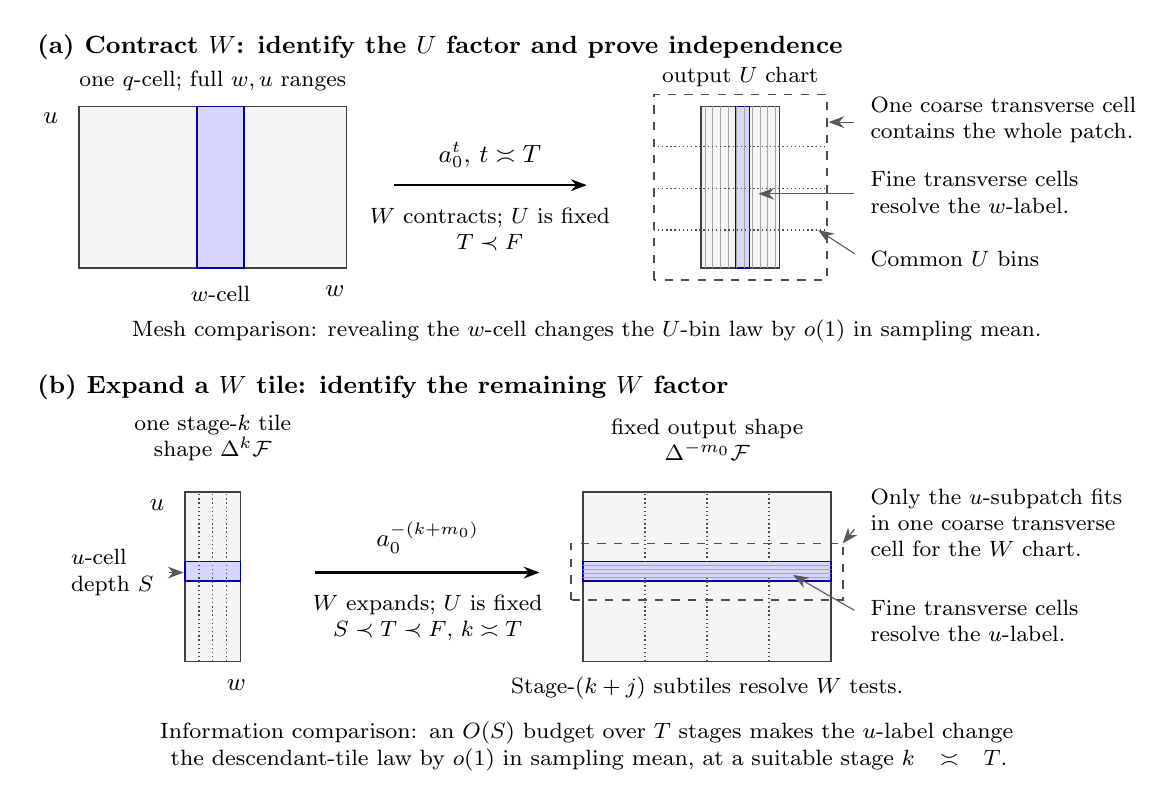
\begin{tikzpicture}[
  x=1cm,y=1cm,
  font=\small,
  >={Stealth[length=2mm]},
  patch/.style={draw=black!75,line width=.55pt,fill=black!4},
  selected/.style={draw=blue!65!black,line width=.55pt,fill=blue!16},
  coarse/.style={draw=black!70,dashed,line width=.65pt},
  fine/.style={draw=black!35,line width=.25pt},
  bins/.style={draw=black!70,densely dotted,line width=.5pt},
  note/.style={align=left,font=\footnotesize},
  leader/.style={draw=black!65,line width=.4pt,->}
]
\path[use as bounding box] (0,-5.15) rectangle (14.2,4.35);

\node[anchor=west,font=\small\bfseries] at (0,4.1)
  {(a) Contract $W$: identify the $U$ factor and prove independence};
\node[align=center,font=\footnotesize] at (2.35,3.67)
  {one $q$-cell; full $w,u$ ranges};
\draw[patch] (.65,1.3) rectangle (4.05,3.35);
\draw[selected] (2.15,1.3) rectangle (2.75,3.35);
\node[font=\footnotesize,anchor=north] at (2.45,1.19) {$w$-cell};
\node[anchor=east] at (.51,3.2) {$u$};
\node[anchor=north] at (3.9,1.19) {$w$};

\draw[->,line width=.8pt] (4.65,2.35) -- (7.1,2.35);
\node[above] at (5.87,2.45) {$a_0^{t}$, $t\asymp T$};
\node[below,font=\footnotesize,align=center] at (5.87,2.18)
  {$W$ contracts; $U$ is fixed\\$T\prec F$};

\draw[coarse] (7.95,1.15) rectangle (10.15,3.5);
\draw[patch] (8.55,1.3) rectangle (9.55,3.35);
\draw[selected] (8.991,1.3) rectangle (9.168,3.35);
\foreach \x in {8.6,8.7,8.8,8.9,9.0,9.1,9.2,9.3,9.4,9.5}
  \draw[fine] (\x,1.3) -- (\x,3.35);
\foreach \y in {1.78,2.31,2.84}
  \draw[bins] (7.95,\y) -- (10.15,\y);
\node[font=\footnotesize] at (9.05,3.73) {output $U$ chart};
\node[note,anchor=west] at (10.58,3.18)
  {One coarse transverse cell\\contains the whole patch.};
\draw[leader] (10.5,3.15) -- (10.17,3.15);
\node[note,anchor=west] at (10.58,2.26)
  {Fine transverse cells\\resolve the $w$-label.};
\draw[leader] (10.5,2.24) -- (9.28,2.24);
\node[note,anchor=west] at (10.58,1.42) {Common $U$ bins};
\draw[leader] (10.5,1.48) -- (10.04,1.78);
\node[align=center,font=\footnotesize] at (7.1,.5)
  {Mesh comparison: revealing the $w$-cell changes the $U$-bin law by $o(1)$ in sampling mean.};

\node[anchor=west,font=\small\bfseries] at (0,-.22)
  {(b) Expand a $W$ tile: identify the remaining $W$ factor};
\node[align=center,font=\footnotesize] at (2.35,-.86)
  {one stage-$k$ tile\\shape $\Delta^k\mathcal F$};
\draw[patch] (2.0,-3.7) rectangle (2.7,-1.55);
\draw[selected] (2.0,-2.68) rectangle (2.7,-2.43);
\foreach \x in {2.175,2.35,2.525}
  \draw[bins] (\x,-3.7) -- (\x,-1.55);
\node[anchor=east] at (1.86,-1.72) {$u$};
\node[anchor=north] at (2.65,-3.81) {$w$};
\node[note,anchor=east] at (1.72,-2.57) {$u$-cell\\depth $S$};
\draw[leader] (1.8,-2.57) -- (1.98,-2.57);

\draw[->,line width=.8pt] (3.65,-2.57) -- (6.5,-2.57);
\node[above] at (5.08,-2.45) {$a_0^{-(k+m_0)}$};
\node[below,font=\footnotesize,align=center] at (5.08,-2.73)
  {$W$ expands; $U$ is fixed\\$S\prec T\prec F$, $k\asymp T$};

\node[align=center,font=\footnotesize] at (8.63,-.88)
  {fixed output shape\\$\Delta^{-m_0}\mathcal F$};
\draw[patch] (7.05,-3.7) rectangle (10.2,-1.55);
\draw[selected] (7.05,-2.68) rectangle (10.2,-2.43);
\foreach \x in {7.8375,8.625,9.4125}
  \draw[bins] (\x,-3.7) -- (\x,-1.55);
\draw[coarse] (6.9,-2.92) rectangle (10.35,-2.2);
\foreach \y in {-2.63,-2.58,-2.53,-2.48}
  \draw[fine] (7.05,\y) -- (10.2,\y);
\node[note,anchor=west] at (10.58,-1.94)
  {Only the $u$-subpatch fits\\in one coarse transverse\\cell for the $W$ chart.};
\draw[leader] (10.5,-2.02) -- (10.35,-2.2);
\node[note,anchor=west] at (10.58,-3.18)
  {Fine transverse cells\\resolve the $u$-label.};
\draw[leader] (10.5,-3.05) -- (9.72,-2.6);
\node[align=center,font=\footnotesize] at (8.63,-4.04)
  {Stage-$(k+j)$ subtiles resolve $W$ tests.};
\node[align=center,font=\footnotesize,text width=14cm] at (7.1,-4.78)
  {Information comparison: an $O(S)$ budget over $T$ stages makes the $u$-label change\\
   the descendant-tile law by $o(1)$ in sampling mean, at a suitable stage $k\asymp T$.};
\end{tikzpicture}
\caption{The two different comparisons in the product rule. Each input picture
fixes a $q$-cell at depth $F$; the coordinate $q$ is suppressed. Dashed outlines
denote coarse output transverse cells; thin solid lines denote fine transverse
cells. Dotted lines denote fixed $U$ bins in (a) and stage-$(k+j)$ $W$ subtiles in (b).
Shading marks a labelled subpatch, not a density. In (a), contraction permits
one coarse transverse-cell comparison for the whole patch and its subpatches.
In (b), expansion leaves the full $U$ interval broad. The full patch is compared
with $V$ data and the thin $u$-subpatch with $W$ data; the information estimate
compares their descendant-tile laws and hence their resolved $W$ tests. All widths and
tile shapes are schematic: $W$ can have several dimensions and its tiles need
not be rectangles. The resulting factor identifications are projective.}
\label{fig:product-mechanism}
\end{figure}


\paragraph{Coverage and the order of choices.}
Fix a permitted exceptional probability \(\epsilon>0\).
Take finitely many input charts
\eqref{eq:simultaneous-product-chart}, with inner boxes and fixed
margins, covering all but a sufficiently small multiple of
\(\epsilon\).  Estimates can be added over these charts; their
finite multiplicity only changes constants.
Use the patches and subpatches just described, with whole
level-\(k\) \(w\)-tiles.  Tiles meeting
the fixed inner boxes lie inside the outer input \(w\) ranges for
large \(i\), because their diameters tend to zero.

First choose a tile-coordinate collar thin enough that its
expected mass is much smaller than the permitted coverage loss.
Lemma~\ref{lem:tiles} does this uniformly in \(k\) and in the input
distribution.  Outside this collar the sample has a fixed
positive margin in \(\mathcal F\).  Choose \(m_0\) so large that
every displacement in a fixed compact set containing
\(\supp f\cup\supp\phi\) and the identity lies, with margin, in
the output tile about such a sample.
Indeed, pull such a displacement back to the input tile
coordinate.  It is contracted by \(\Delta^{m_0}\); the
conjugation coming from the input \(u\) coordinate is uniformly
bounded, and commutes with \(\Delta\), since \(a_0\) fixes \(U\).
Thus the pulled-back displacement fits inside the chosen margin
for sufficiently large fixed \(m_0\).
The input inner \(u\) intervals also give a fixed \(U\)
neighborhood about the sampled output point.

Now take finitely many output charts of the same simultaneous
form, with inner boxes and \(V\)-extensions large enough for the
images of these patches.  Such a finite cover loses an arbitrarily
small further probability.  For fixed \(m_0\), all displacements
from a sample to points in its output patch lie in a fixed compact
range: use the tile origin as base in \(W\), a fixed base in \(U\),
and the fixed shape \(\Delta^{-m_0}\mathcal F\).
The \(q\) variation after \eqref{eq:reverse-motion} is
\(O(2^{-F}e^{CT})\).
Hence a patch meeting an output inner box fits in its extended
chart with margin.  We can assign these patches to the finitely
many output charts, or perform the estimates for each applicable
input--output pair.  We keep only samples with the indicated
inner margins.

These choices fix the chart cover, the output tile extent, and
the test-range margins.  They do \emph{not} yet fix the accuracy
of bin comparisons.  Afterwards one may make a second,
arbitrarily thinner tile-boundary exclusion, refine the fixed
output bins, and increase the fixed integer \(j\).  These later
choices improve errors without changing the earlier coverage
requirements.

All these requirements can be met simultaneously with the
information estimate.  Initially average both over shifts and
over \(k\in[T/2,3T/4]\).  The first collar was chosen to have
expected loss small enough that its required coverage bound
holds with high probability.  Any later, finer collar can have
arbitrarily small expected loss.  For every fixed \(j\),
Lemma~\ref{lem:stage-information} gives an error tending to zero
in this joint average.  Markov's inequality therefore selects
common shifts and \(k=k_i\) satisfying the coverage bounds and
the desired comparison-error bounds.  The transverse grids in
\(q,u\) may be fixed using the grid convention of the preceding
section.  Every scale still satisfies
\eqref{eq:w-factor-scales}.

\paragraph{Geometry of the output comparisons.}
Write the coordinates of an assigned output chart as
\((q',w',u')\).  For fixed input \(q\), its patch image is obtained
by left multiplication in \(V\) from
\[
                     \Delta^{-m_0}\mathcal F
                            \ \times\ (\text{input }u\text{ interval}).
\]
Left multiplication by \(w_0u_0\) sends \(wu\) to
\begin{equation}\label{eq:separate-left-translation}
                   \bigl(w_0\Ad_{u_0}(w)\bigr)\,(u_0u).
\end{equation}
Thus the two plaque coordinates change separately.  The
parameters of this bounded left multiplication vary by
\(O(2^{-F}e^{CT})\) across the input \(q\)-cell.
The \(V\)-transverse diameter in \(q'\) is bounded by the same
quantity.  It is smaller than \(2^{-CS}\) for every fixed \(C\)
when \(i\) is large.
For a subpatch, the \(W\)-transverse coordinates are
\((q',u')\); their diameter is
\[
                         O(2^{-S}+2^{-F}e^{CT})
                                  =o(2^{-l_-}).
\]
Discard patches or subpatch comparisons crossing a coarse
output transverse wall.  Their sampling mass is \(o(1)\).

We apply Lemma~\ref{lem:patch-comparison} to \(V\) data on the
patches and \(W\) data on the subpatches.  The needed inner
products are as follows.  For a patch take collections of
\(w'\) and \(u'\) bins in product form; for each of its subpatches
use the same inner collection of \(w'\) bins.  These collections
are admitted over the entire corresponding transverse
projection, by \eqref{eq:separate-left-translation} and the
vanishing variation of its parameters.

We verify that these inner products lose as little sampling
mass as desired.  The extended charts describe one plaque sheet
throughout each of the ranges involved.  The transverse maps
are injective on a patch or subpatch: their images have a common
open plaque range, and injectivity follows from injectivity of
the original chart and the diagonal motion.  Vary a fine output
transverse coordinate across its cell and pull the path back.
Its input length is at most \(e^{CT}\) times the fine mesh side.
Because \(F,S\prec l_+\), this path stays in its input \(q\)- and
\(u\)-cells except at grid-wall collars of mass \(o(1)\).
Fixed input chart-boundary collars have arbitrarily small mass.
In tile coordinates the same pullback costs at most \(e^{C'T}\),
so it stays in the input tile away from any fixed thin collar
of that tile's boundary.  The second collar chosen above makes
this loss arbitrarily small.

Finally, away from these collars, the sample has a definite
margin in its admitted \(w'\) and \(u'\) ranges.  For \(w'\) the
margin depends on \(m_0\), the fixed charts, and the tile
collar thickness; for \(u'\) it follows from the fixed interval
margin.  Sufficiently fine fixed plaque bins are then wholly
admitted.  This proves the required plaque-bin trim estimate.
The collections can retain the supports of \(f,\phi\) about
the covered samples and a fixed \(U\) neighborhood about their
\(u'\) coordinates.  Thus the comparison errors can be made
arbitrarily small after the original coverage and range choices.

\paragraph{Comparison of the \(W\) tests.}
At a sampled output point, let \(P_V\) and \(P_W\) denote its
finite-\(i\) chart probabilities for \(V\) and \(W\).
Interpret \(f,\phi\) in the output \(w'\) coordinate using the
displacement formula \eqref{eq:product-displacement}.  Their
parameters may depend on the sample, but their norms and
continuity moduli are uniform on the finitely many chart ranges.
Let \(B_u\) denote the union of the inner \(u'\) bins for its
patch.  We claim that, on the covered samples,
\begin{equation}\label{eq:w-cross-product}
             P_V(f\,1_{B_u})P_W(\phi)
                    -P_V(\phi\,1_{B_u})P_W(f)
\end{equation}
has arbitrarily small expectation of its absolute value in the
limit \(i\to\infty\).

Here is the mass calculation.  Let \(A_p\) be the law of the
output plaque coordinates when sampling the input patch \(p\),
and let \(A_{p'}\) be the corresponding law for its subpatch.
The unnormalized form of Lemma~\ref{lem:patch-comparison},
first for \(V\) and then for \(W\), gives
\[
 \begin{aligned}
       c_p A_p(f)&\simeq P_V(f\,1_{B_u}),&
       c_p A_p(\phi)&\simeq P_V(\phi\,1_{B_u}),\\
       c_{p'} A_{p'}(f)&\simeq P_W(f),&
       c_{p'} A_{p'}(\phi)&\simeq P_W(\phi).
 \end{aligned}
\]
Let \(e_f(x),e_\phi(x),e'_f(x),e'_\phi(x)\) denote the absolute
errors in these four comparisons at the sampled point \(x\).
The factors \(c_p,c_{p'}\) are the probabilities of the admitted
plaque-bin ranges in the respective coarse output laws, hence
belong to \([0,1]\).  Each \(\simeq\) means an absolute error whose
sum weighted by the relevant patch masses is arbitrarily small.
The tests are supported in the common inner \(w'\) range, so
there is no additional \(w'\)-restriction in the right-hand
integrals.  Replacing coarse laws by the data laws uses the
plateau comparison.  These estimates remain true for the
sample-dependent test parameters by the uniform-test clause
of Lemma~\ref{lem:patch-comparison}.

At input, Lemma~\ref{lem:stage-information} compares the law of
the level-\((k+j)\) tile in \(p\) with its law in \(p'\).
At output these finer tiles have relative shapes
\(\Delta^{j-m_0}\mathcal F\).  Once \(m_0\) and the finite chart
ranges are fixed, taking the fixed integer \(j\) large makes
their diameters as small as prescribed.  The conversion to
\(w'\) coordinates has uniformly bounded distortion and is
independent of \(u\), by
\eqref{eq:separate-left-translation}.
Let \(\eta_i(x)\) be the \(\ell^1\) distance between the two
conditional level-\((k+j)\) tile laws for the patch and the
subpatch containing \(x\).  There is a uniform bound
\[
 \sigma_{i,j}
    \le C\,\diam(\Delta^{j-m_0}\mathcal F)+O(2^{-F}e^{CT})
\]
for the variation of \(w'\) within one such tile, including the
variation across its \(q\)-cell.  If \(h\) is either \(f\) or
\(\phi\), and \(\omega_h\) is a common continuity modulus for its
chart-coordinate versions, then
\begin{equation}\label{eq:tile-test-comparison}
       |A_p(h)-A_{p'}(h)|
                  \le \eta_i(x)+2\omega_h(\sigma_{i,j}).
\end{equation}
Indeed, replace \(h\) by one value on each finer tile.  The two
replacements cost at most \(\omega_h(\sigma_{i,j})\) each, and
the remaining finite-label difference is bounded by \(\eta_i(x)\).
This also proves the assertion for tests based at the sampled
point, since the bound is uniform over the test coefficients.
The expected value of \(\eta_i\) tends to zero for the selected
shifts and stages, by Lemma~\ref{lem:stage-information}.

Multiply the four mass comparisons and cancel by cross
multiplication, without dividing by \(c_p\) or \(c_{p'}\).
The result is \eqref{eq:w-cross-product}: the remaining expression
is bounded by
\[
 \begin{split}
 &e_f(x)+e_\phi(x)+e'_f(x)+e'_\phi(x)\\
 &\hspace{15mm}
       +2\eta_i(x)
       +2\omega_f(\sigma_{i,j})+2\omega_\phi(\sigma_{i,j}).
 \end{split}
\]
For this inequality, the term left after the four mass
comparisons is
\(c_pc_{p'}(A_p(f)A_{p'}(\phi)-A_p(\phi)A_{p'}(f))\);
apply \eqref{eq:tile-test-comparison} and use that all factors
are bounded by one.
Integrating over the covered samples bounds
the first four terms by the total trim and bin-comparison
errors, the fifth by the stage-information error, and the last
two by their uniform moduli.  Choose the trim accuracy and fixed
bins first, then choose the fixed \(j\) sufficiently large, and
finally let \(i\) tend to infinity.
This proves the claimed integrated bound for
\eqref{eq:w-cross-product}.
The number of patches may grow with \(i\); the absolute mass estimate
\eqref{eq:mass-error} charges each fine-cell/bin pair at most
once within a fixed chart comparison.

\paragraph{Removing the \(U\) restriction.}
By Lemma~\ref{lem:u-factor}, in the limiting \(V\) data the
\(w'\) and \(u'\) coordinates are independent.  Consequently,
for the finite-\(i\) probabilities,
\[
       P_V(f1_{B_u})-P_V(f)P_V(B_u)\longrightarrow0
\]
in probability on the charts under consideration, and the same
holds with \(\phi\).  To justify the varying \(B_u\), its bins
come from one fixed finite subdivision, and every bin boundary
has zero mass almost surely in the limiting data.  The asserted
convergence therefore holds simultaneously for all subsets of
that finite bin collection.  The displacement tests depend
continuously on the sample on the fixed inner chart ranges.
Output sampling has law \(\mu_i\), so the limiting independence
applies there even though the patches were chosen at input.
If several input charts are used, their finite multiplicity
only multiplies the error bound.

Thus \eqref{eq:w-cross-product} becomes
\begin{equation}\label{eq:w-cross-product-reduced}
 P_V(B_u)
       \bigl(P_V(f)P_W(\phi)-P_V(\phi)P_W(f)\bigr)
                            \simeq0.
\end{equation}

\paragraph{Denominators and passage to the projective limit.}
We now explain why \eqref{eq:w-cross-product-reduced} gives
\eqref{eq:w-ratio-target}.  On each of the fixed covered chart
ranges, \(B_u\) contains a fixed \(U\) neighborhood about the
sample.  Choose a continuous bump supported in that neighborhood
and positive at the sampled \(u'\) coordinate.  Its integral in
the limiting \(V\) probability is positive by identity support.
The same support property gives positivity of the limiting
integrals \(P_V(\phi)\) and \(P_W(\phi)\).
For any further prescribed exceptional probability there is,
therefore, a constant \(\kappa>0\) such that, for all large \(i\),
\begin{equation}\label{eq:w-denominators}
          P_V(B_u)\ge\kappa,\qquad
          P_V(\phi)\ge\kappa,\qquad
          P_W(\phi)\ge\kappa
\end{equation}
outside that exception on the covered samples.
This follows from convergence of the joint data in the finitely
many charts, using the fixed continuous bumps.

The order of choices is essential.  Fix the coverage, \(m_0\),
the output charts, and their test-range margins first.  Then
choose \(\kappa\) from these fixed bumps.  Only afterwards refine
the bin approximations and tile collars used for comparison,
and enlarge \(j\), to make the error in
\eqref{eq:w-cross-product-reduced} as small as required relative
to \(\kappa^3\).  The coverage collar and the fixed neighborhoods
giving the lower bounds need not change.  Division in
\eqref{eq:w-cross-product-reduced} is now legitimate and yields
arbitrarily small difference between
\[
                         \frac{P_V(f)}{P_V(\phi)}
                 \quad\hbox{and}\quad
                         \frac{P_W(f)}{P_W(\phi)}
\]
outside an arbitrarily small exceptional probability.
Explicitly, let \(\mathcal G_i\) be the covered set on which
\eqref{eq:w-denominators} holds, and denote the expression on the
left of \eqref{eq:w-cross-product-reduced} by \(D_i(x)\).
For every \(\delta>0\),
\[
 \mu_i\left(\mathcal G_i\cap
   \left\{\left|\frac{P_V(f)}{P_V(\phi)}
                -\frac{P_W(f)}{P_W(\phi)}\right|>\delta\right\}\right)
       \le \frac{1}{\delta\kappa^3}
                \int_{\mathcal G_i}|D_i(x)|\,\dd\mu_i(x).
\]
The right side can be made arbitrarily small with the previously
fixed coverage and denominators.

To see that this proves the assertion for the limiting
projective measures, suppose otherwise.  A countable choice of
tests and charts would then give a reference output chart and
a positive-probability set on which the two ratios differ by
more than some fixed positive number.  Restrict this set so
that the denominators have a positive lower bound and the
supports of the tests, together with a \(U\) neighborhood, have
inner margins in the chart.  Continuous displacement integrals
and the open-set inequality preserve a positive probability
of discrepancy in the sequence data.

Apply the preceding coverage construction with exceptional
probability much smaller than this discrepancy probability.
On samples covered by both the reference chart and an assigned
output chart, Proposition~\ref{prop:plaque-comparison} and
Lemma~\ref{lem:u-factor} identify their limiting ratios.
This also identifies their finite-\(i\) ratios up to an error
tending to zero outside a further small set: first impose
closed inner margins and lower bounds on the denominators,
then use joint convergence of the finitely many chart data.
The arbitrarily accurate comparison just proved in the
assigned charts contradicts persistence of the discrepancy
in the reference chart.

We have proved \eqref{eq:w-ratio-target}.  Taking countably many
tests and then exhausting compact \(W\) ranges gives
\(\nu^W_\omega\propto m^W_\omega\) almost surely.
Together with \eqref{eq:provisional-product}, this completes
the proof of Theorem~\ref{thm:product}.

\section{Active roots and their support}\label{sec:activity}

The product rule turns the plaque measures into a directed graph at each
augmented state.  We first show that its arrows compose and describe the
support of the positive-root plaques.  We then realize this graph by
measurable indicators on the original spaces, retaining the long-wall
comparison needed for the entropy argument.

Write $\mathsf P$ for the law of the limiting augmented state
$\omega=(x,(P^B)_B)$.  For $j\ne k$, define
\[
 a_{jk}(\omega)
   =\mathbf 1_{\{m^{U_{jk}}_\omega\text{ is not supported on }\{1\}\}}.
\]
We call $jk$ \emph{active} when $a_{jk}=1$.  This definition does not depend
on the representative of the projective measure.  It is measurable:
after normalizing by a positive integral against a bump near the identity,
activity is detected by a countable family of nonnegative continuous
tests supported away from the identity.  All assertions below are made
on a common set of full $\mathsf P$-measure on which the comparison and
product rules hold.

\begin{proposition}[Composition and positive-root support]
\label{prop:activity}
Almost surely, activity is transitively closed:
\[
 a_{pq}(\omega)a_{qr}(\omega)
       \bigl(1-a_{pr}(\omega)\bigr)=0
       \qquad(p,q,r\text{ distinct}).
\]
Let $b\in L$ be regular, let $V$ be the pattern group of all
$b$-positive roots, and let $V_\omega^+$ be the subgroup generated by
the active $b$-positive root groups.  These active roots form a pattern,
and
\[
                   \supp m^V_\omega\subset V_\omega^+.
\]
Both conclusions hold simultaneously for every regular $b$.
\end{proposition}

\begin{proof}
First observe that Theorem~\ref{thm:product} factors the measure of any
pattern group into its one-dimensional root measures, in a suitable
order.  Indeed, the cone generated by its roots is pointed.  Choose a
root $\alpha$ on an exposed extremal ray.  No other root in the pattern
is proportional to $\alpha$, so a diagonal logarithm can vanish on
$\alpha$ and be strictly negative on every remaining root.  Removing
$\alpha$ leaves a normal pattern subgroup $W$: a sum of two roots in
the original pattern cannot equal $\alpha$, since extremality would
force both summands onto its ray.  Thus the hypotheses of
Theorem~\ref{thm:product} hold for $V=WU_\alpha$.  Iterate, allowing
$W=\{1\}$ at the last step.

To prove transitivity, fix distinct $p,q,r$ and consider the
three-root Heisenberg group generated by $U_{pq},U_{qr},U_{pr}$.
Suppose that $a_{pr}=0$.  Factoring first with $U_{pq}$ as the final
factor, and then with $U_{qr}$ as the final factor, gives two
descriptions of the same projective measure.  Write
$u_{jk}(t)=1+tE_{jk}$.  Since the $U_{pr}$ factor is a point mass, the
first description is supported on the matrices
\[
 u_{qr}(t)u_{pq}(s)=1+sE_{pq}+tE_{qr},
\]
whereas the other is the pushforward of the product of the two root
measures under
\[
 u_{pq}(s)u_{qr}(t)
     =1+sE_{pq}+tE_{qr}+stE_{pr}.
\]
If both roots were active, each root measure would give positive mass
to some compact parameter set disjoint from zero.  Their product would
then give positive mass to matrices with nonzero $pr$ entry, contrary
to the first description.  The projective identities apply on compact
ranges containing these sets, so all masses used here are finite.
This proves transitivity.

For the support assertion, use the successive factorization already
proved.  Every inactive root factor is a point mass at the identity;
every other factor is supported on its own active root group.  The
product is therefore supported on the subgroup generated by the active
roots.  Transitivity says exactly that the active positive roots are
closed under root addition, so this subgroup is a pattern group and is
closed.  There are only finitely many positive-root patterns, which
also gives the simultaneous assertion.
\end{proof}

The entropy argument will use plaques enlarged by the diagonal group.
The following consequence retains the activity at the sampled state.

\begin{lemma}[Support on plaques enlarged by $A$]\label{lem:va-support}
With $V$ and $V_\omega^+$ as in Proposition~\ref{prop:activity}, the
limiting $VA$-plaque probability, written in displacement coordinates
from its sampled point, is supported on $V_\omega^+A$ within its chart.
\end{lemma}

\begin{proof}
Use a product box with coordinates $\psi(q)va$, with product coordinate
domains.  Local $A$-invariance gives, for each $i$, a product
decomposition
\[
                d\mu_i(q,v,a)=d\nu_i(q,v)\,da
\]
inside the box, where $da$ is Haar measure restricted to its coordinate
box and the normalization is absorbed into $\nu_i$.  For $VA$ plaques
the transverse coordinate is $q$; for $V$ plaques it is $(q,a)$.
Choose a common $q$ grid and supplement it by an $a$ grid for the latter
conditioning.  Conditional on a $q$ cell, the $VA$ probability is the
product of a probability on $v$ and normalized Haar measure on $a$.
Conditioning also on an $a$ cell leaves the $v$ probability unchanged.
These are exact identities before taking a limit.  The interior-depth
comparisons permit these compatible grids in the defining data, and
the identities pass to the joint limit by continuous tests and the
null-boundary convention.

At a sample $x=\psi(q_s)v_sa_s$, the $V$ displacements corresponding to
varying $v$ at fixed $a_s$ are
\[
                         a_s^{-1}v_s^{-1}va_s.
\]
By Proposition~\ref{prop:activity}, their probability is supported on
$V_\omega^+$.  A general $VA$ displacement is
\[
 a_s^{-1}v_s^{-1}va
   =\bigl(a_s^{-1}v_s^{-1}va_s\bigr)\bigl(a_s^{-1}a\bigr),
\]
and hence belongs to $V_\omega^+A$ almost surely.  The argument applies
on inner chart boxes; exhausting them gives the statement on the whole
plaque box, whose boundary has zero probability.
\end{proof}

\begin{lemma}[Indicators along the sequence]\label{lem:activity-indicators}
Fix an interior scale $R_i$ allowed in the long-wall comparison of
Proposition~\ref{prop:plaque-comparison}, with ratio-separated depths on
both sides of it inside $(l_{-,i},l_{+,i})$.  There exist measurable
functions $g_{jk,i}:X\to\{0,1\}$ such that
\[
 \operatorname{Law}_{\mu_i}\bigl(Z_i(x),(g_{jk,i}(x))_{j\ne k}\bigr)
 \ \Longrightarrow\
 \operatorname{Law}_{\mathsf P}
       \bigl(\omega,(a_{jk}(\omega))_{j\ne k}\bigr).
\]
They satisfy asymptotic transitivity:
\[
 \int_X g_{pq,i}(x)g_{qr,i}(x)
                  \bigl(1-g_{pr,i}(x)\bigr)\,d\mu_i(x)=o(1)
       \qquad(p,q,r\text{ distinct}),
\]
and, for every fixed $C<\infty$,
\begin{equation}\label{eq:wall-invariance}
 \sup_{\substack{b\in\ker\beta_{jk}\\ \|b\|\le CR_i}}
 \int_X\bigl|g_{jk,i}(xa(b))-g_{jk,i}(x)\bigr|\,d\mu_i(x)
                         \longrightarrow0.
\end{equation}
\end{lemma}

\begin{proof}
Let $\mathcal S$ be the separable metric state space used for $Z_i$,
and put $A_{jk}=\{\omega:a_{jk}(\omega)=1\}$.  Choose
$\epsilon_r\downarrow0$.  For each root and each $r$, there is a
$\mathsf P$-continuity set $D_{jk,r}\subset\mathcal S$ such that
\[
              \mathsf P(D_{jk,r}\mathbin\triangle A_{jk})
                      <\epsilon_r.
\]
For completeness, use a countable family of continuous coordinate
tests generating the Borel sets of $\mathcal S$.  For each test choose
a countable dense family of thresholds outside the atoms of its
distribution under $\mathsf P$.
The finite Boolean combinations of the resulting threshold sets have
null boundary and approximate every measurable set in
$\mathsf P$-measure.  Thus the approximations may be made using
finitely many data tests at each stage.

For fixed $r$, set
$g^{(r)}_{jk,i}(x)=\mathbf 1_{D_{jk,r}}(Z_i(x))$.
Weak convergence of the states and the null boundaries give joint
convergence of the states and these finitely many indicators.  Since
the exact indicators are transitive, the limiting transitivity defect
for any triple is at most $3\epsilon_r$.

We next prove the uniform wall estimate at this fixed approximation
level.  Fix a root, $C$, and any sequence
$b_i\in\ker\beta_{jk}$ with $\|b_i\|\le CR_i$.  Both marginals of
\[
                    \bigl(Z_i(x),Z_i(xa(b_i))\bigr)
\]
have the ordinary state law, because $\mu_i$ is $A$-invariant.
Consequently these paired laws are tight.  In every subsequential
limit their two marginals are $\mathsf P$, and
Proposition~\ref{prop:plaque-comparison} identifies the two projective
$U_{jk}$ measures.  Their exact activity indicators are therefore
equal.  Applying the continuity-set approximation separately in the
two marginals shows that every such limit has
\[
 \mathbb E\bigl|
       \mathbf 1_{D_{jk,r}}(\omega)
        -\mathbf 1_{D_{jk,r}}(\omega')\bigr|
                    \le 2\epsilon_r.
\]
The boundary of the tested event is contained in the union of the two
marginal boundaries, so the corresponding prelimit expectations
converge along this subsequence.  Since the sequence $b_i$ was
arbitrary, a sequence chosen within a vanishing error of the supremum
proves
\[
 \limsup_i\ \sup_{\substack{b\in\ker\beta_{jk}\\\|b\|\le CR_i}}
 \int_X\bigl|g^{(r)}_{jk,i}(xa(b))-g^{(r)}_{jk,i}(x)\bigr|\,d\mu_i(x)
                      \le2\epsilon_r.
\]
This argument uses limits of paired states even when $b_i$ diverges.

Finally choose $r=r(i)\to\infty$ sufficiently slowly.  At stage $r$
impose the preceding estimates for all roots, all triples, and all
integers $1\le C\le r$, together with the first $r$ tests of a
convergence-determining family for the joint state and indicator law.
The limiting laws at fixed $r$ differ from the exact activity law by
at most the sum of the finitely many approximation errors.  A
diagonal choice therefore gives the asserted joint convergence,
vanishing transitivity defects, and \eqref{eq:wall-invariance} for
$g_{jk,i}=g^{(r(i))}_{jk,i}$.  Bounds for integral $C$ imply the bounds
for every fixed finite $C$.
\end{proof}

We conclude with the relation between activity and pieces having
countable intersections with root plaques.
It is this relation that will exclude proper homogeneous components
once all roots have been shown to be active.

\begin{lemma}[Inactivity on pieces with countable plaque sections]\label{lem:transverse-inactive}
Let $S\subset X$ be a Borel set whose intersection with each local
$U_{jk}$ plaque is countable.  Then
\[
            a_{jk}(\omega)=0
         \quad\text{for $\mathsf P$-almost every state with }x\in S.
\]
In particular, this applies to the fixed-point pieces of
Lemma~\ref{lem:fixed-pieces} for roots crossing distinct eigenvalues:
each such piece meets a sufficiently small root plaque in at most one
point.  It also applies to countable unions of these pieces.
\end{lemma}

\begin{proof}
Work first in a $U_{jk}$ flow box with coordinates $(q,h)$ and plaque
probability $P^B$.  For each $q$, the section
\[
                  S_q=\{h:\psi(q)h\in S\}
\]
is countable.  The sampling identity for this single chart states
that the conditional law of the sampled $h$, given $(q,P^B)$, is
$P^B$.  A probability measure assigns mass zero to those points of a
countable set which are not its atoms.  Consequently
\[
 \mathsf P\{x\in S\cap B,\ P^B(\{h\})=0\}=0.
\]
No conditioning on the other plaque probabilities is used here.
Projective agreement in the chart identifies an atom at the sampled
$h$ with an atom at the identity of $m^{U_{jk}}_\omega$.  A countable
flow-box cover therefore shows that this root measure has an atom at
the identity almost surely over $S$.

It remains to show that, under the full state law, an atom at the
identity forces the entire root measure to be supported there.
Identify $U_{jk}$ with $\R$ by $t\mapsto1+tE_{jk}$.  Choose a fixed
$b\in L$ with $\lambda=e^{\beta_{jk}(b)}>1$.  Fixed-motion equivariance
in Proposition~\ref{prop:plaque-comparison}, together with
$A$-invariance of the prelimit sampling law, says that the projective
law of $m^{U_{jk}}_\omega$ is invariant under the pushforward by
$t\mapsto\lambda t$.

The event that this measure has an atom at zero is itself invariant
under dilation.  If that event has positive probability, condition
the projective-measure law on it and normalize each measure $m$ by
its atom: $\nu=m/m(\{0\})$.  This is a measurable normalization of a
locally finite measure, with $\nu(\{0\})=1$, and its law remains
dilation-invariant.  For every compact interval $K$ disjoint from
zero,
\[
 (t\mapsto\lambda^n t)_*\nu(K)
         =\nu(\lambda^{-n}K)\longrightarrow0.
\]
Indeed, $\lambda^{-n}K$ lies in a shrinking punctured neighborhood of
zero, whose mass tends to zero by local finiteness.  Dilation
invariance makes each quantity in this display have the same
distribution as $\nu(K)$.  Almost-sure convergence to zero therefore
forces $\nu(K)=0$ almost surely.  A countable family of such intervals
covers $\R\setminus\{0\}$, and hence $\nu=\delta_0$ almost surely.
The atom event of probability zero is harmless.  Combining this
conclusion with the first part proves the lemma.
\end{proof}

\section{Activity along long diagonal segments}\label{sec:segment-entropy}

The root probabilities constructed above detect variation within a plaque at
the intermediate resolutions.  We now use the arithmetic tube estimate to
show that this variation cannot disappear across a cut for a positive
proportion of starting points over a long diagonal segment.  A positive
average under $\mu_i$ alone could coexist with zero activity on a set of
starting points of positive measure.  If $\mu_i(E_i)\geq p>0$, the
normalized restrictions $\xi_i=\mu_i|_{E_i}/\mu_i(E_i)$ satisfy
$\xi_i\leq p^{-1}\mu_i$.  Proving the estimate for every such dominated
law excludes these positive-mass exceptional sets.  In
Section~\ref{sec:combination}, this stronger conclusion will give
almost-sure segment positivity for the limiting functions.

An \emph{oriented cut} is a nonempty proper subset
$J\subset\{1,\ldots,6\}$, with the roots directed from $J$ to its complement:
\[
 \mathcal E_J=\{\beta_{jk}:j\in J,\ k\notin J\}.
\]
The complementary subset gives the opposite orientation.  Fix a small
$\delta>0$.  For each such $J$, choose a regular $b_J\in L$ such that
\begin{equation}\label{eq:cut-direction}
 \beta(b_J)\geq1\quad(\beta\in\mathcal E_J),\qquad
 |(b_J)_k-(b_J)_j|\leq\delta
 \quad(j,k\text{ on the same side of }J).
\end{equation}
These choices can be made in a fixed bounded subset of $L$: put the two
sides at two distinct levels, perturb the entries within each side, and
subtract their common average.  There are only finitely many cuts.
Write $\eta=1/3$ for the exponential constant in
Proposition~\ref{prop:bowen}; it is independent of $\delta$.
Write $g_{\beta,i}=g_{jk,i}$ when $\beta=\beta_{jk}$, and put
\[
 A_{J,i}(x)=\sum_{\beta\in\mathcal E_J}g_{\beta,i}(x).
\]
Choose the common interior scale $R_i$ as in
\eqref{eq:wall-invariance}, leaving separated interior depths both below and
above it.  In particular, $T_{-,i}\prec R_i\prec T_{+,i}$.

\begin{proposition}[Activity on every long segment]\label{prop:segment-activity}
For $\delta$ sufficiently small, the preceding choices have the following
property.  For every oriented cut $J$, every $C<\infty$, every $\tau>0$,
and every sequence of probabilities $\xi_i$ on $X$ satisfying
$\xi_i\leq C\mu_i$,
\begin{equation}\label{eq:segment-activity}
 \liminf_{i\to\infty}\frac1{R_i}
 \int_0^{\tau R_i}\int_X
 A_{J,i}\bigl(xa(tb_J)\bigr)\,\dd\xi_i(x)\,\dd t>0.
\end{equation}
The same assertion holds after passage to any subsequence.
\end{proposition}

The proof compares two bounds for the entropy of orbit names.  The tube
estimate gives a positive entropy cost per unit time.  If the roots crossing
the cut are inactive, the plaque probabilities vary only in directions
whose expansion rates are at most $\delta$.  Their names then have a much
smaller coding cost.  This use of arithmetic separation to bound the entropy
of diagonal orbit names belongs to the method of
\cite{ELMV2009}; here the conditioning at intermediate resolutions and the
arbitrary dominated starting probabilities require the additional details
below.  We use Shannon entropy with natural logarithms, including its chain
rule and the elementary finite-alphabet error bound; see
\cite[Chapter~2]{CoverThomas2006}.

\subsection{Partitions and the cusp}

For a countable partition $\mathcal P$ and a probability $\nu$, write
\[
 H_\nu(\mathcal P)=-\sum_{P\in\mathcal P}\nu(P)\log\nu(P),
 \qquad 0\log0=0.
\]
Fix a regular $b\in L$ and put $T(x)=xa(b)$.  The notation
$\mathcal P_{[r,s]}=\bigvee_{t=r}^sT^{-t}\mathcal P$ records the symbols at
the integer times from $r$ through $s$.  Let $V$ be the pattern group of
the $b$-positive roots.

\begin{lemma}[A partition for consistent orbit names]\label{lem:entropy-partition}
Given a sufficiently small identity neighborhood $O\subset G$, there is a
countable Borel partition $\mathcal P$ of $X$ with the following properties.
\begin{enumerate}
 \item Every atom has $\mu$-null boundary and lies in an inner part of a
 relatively compact $VA$ plaque chart from the fixed stock.  The chart
 extends beyond the atom with a margin.
 \item If $x,y$ have the same symbols at times $0,\ldots,N$, there are
 relative lifts $h_t\in O$, $0\leq t\leq N$, such that
 \[
  ya(tb)=xa(tb)h_t,
  \qquad h_{t+1}=a(-b)h_ta(b).
 \]
 \item For every fixed $C$, the entropies $H_\nu(\mathcal P)$ are bounded
 uniformly for all sufficiently large $i$ and all probabilities
 $\nu\leq C\mu_i$.  Moreover, there are finite coarsenings
 $\mathcal P^{(q)}$, obtained by keeping finitely many atoms and combining
 the others into one atom, for which
 \begin{equation}\label{eq:partition-entropy-tails}
  \lim_{q\to\infty}\limsup_{i\to\infty}
  \sup_{\nu\leq C\mu_i}
  H_\nu(\mathcal P\mid\mathcal P^{(q)})=0.
 \end{equation}
\end{enumerate}
\end{lemma}

\begin{proof}
Let $m(x)$ denote the shortest-vector length.  Divide $X$ into layers on
which $m(x)$ is comparable to $e^{-k}$, for integers $k\geq0$, using a
first layer that also contains the thick part.  Layer boundaries may be
chosen $\mu$-null.  Successive minima and lattice basis reduction give a
representative matrix $g$ for each point of the $k$th layer such that
\[
 \|g\|+\|g^{-1}\|\leq e^{C_1(1+k)}.
\]
Consequently the injectivity radius for relative group coordinates on that
layer is at least $e^{-C_2(1+k)}$.  Indeed, if a nonidentity integral matrix
$\gamma$ gave a smaller return, conjugating the return by $g$ would give
$\|\gamma-1\|<1$, which is impossible.

We impose a quantitative margin condition on these charts.  Write $d_G$
for the fixed left-invariant Riemannian distance on $G$.  In a fixed
identity neighborhood of $G$, adapted product coordinates give a smooth
retraction $\pi$ onto $VA$, with $\pi(h)=h$ for $h\in VA$ and
\[
 d_G(h,\pi(h))\leq C_{\pi}\dist_G(h,VA),
 \qquad d_G(1,\pi(h))\leq C_{\pi}d_G(1,h).
\]
After shrinking the neighborhood, $1$ and $\pi(h)$ are joined inside
$VA$ by a path of length at most $C_{\pi}d_G(1,h)$; one may use the
local exponential coordinates of $VA$.

Choose outer $VA$ product charts in the $k$th layer of radius comparable
to $r_k=e^{-C_3(1+k)}$, with $C_3$ sufficiently large for injectivity,
and inner boxes whose relative-coordinate distance from the outer
boundary is at least a fixed multiple of $r_k$.  Use translates of a
fixed smooth group-coordinate chart, so that its local product and
metric comparison constants are uniform.  Cover the layer by still
smaller symbol boxes inside these inner boxes.  Require their
relative-group diameter to be at most $c_*r_k$, where $c_*>0$ is small
enough compared with both the inner-to-outer margin and the radius of
the domain of $\pi$.  In particular, whenever $x,y=xh$ are in one
symbol box, the whole path from $x$ to $x\pi(h)$ just described stays
inside its outer chart.  It follows that $x\pi(h)$ is on the same
chart plaque as $x$, rather than on another local sheet of that orbit.

The number of symbol boxes needed is at most $e^{C_4(1+k)}$.
Indeed, subdivide the bounded-matrix representatives at an exponentially
small mesh, and refine by the fixed factor $c_*$ when necessary.  These
operations preserve an exponential bound in $k$.  Passing from the cover
to a partition by successive differences does not increase the number
of pieces or their diameters.  The charts and their cuts can be chosen
from the stock with $\mu$-null boundaries: perturb centers within a small
fixed fraction of the covering radius and choose each coordinate width
in a fixed comparable interval, avoiding the at most countably many
widths that give a boundary of positive measure.  These choices preserve
the exponential bounds on sizes and on the number of boxes, as well as
the inner-chart margins.  Thus each partition atom remains
inside a chart with a margin, although it need not itself be a coordinate
rectangle.

The shortest-vector length changes by at most a fixed multiplicative factor
under $T$.  We can therefore choose the boxes so small that both a relative
lift in one symbol and its conjugate by $a(b)$ lie in an injective
neighborhood at the next symbol.  Uniqueness in that neighborhood identifies
the latter lift with the lift chosen there.  Induction gives the consistency
in assertion~2.  Decreasing all box sizes by a common fixed factor ensures
that every lift lies in the prescribed $O$.

By Proposition~\ref{prop:cusp}, a probability $\nu\leq C\mu_i$ assigns the
$k$th layer mass at most $C_5e^{-c k}$, uniformly for sufficiently large
$i$.  If that mass is $p_k$ and there are at most $M_k$ symbols in the
layer, their entropy is bounded by
\[
 p_k\log M_k-p_k\log p_k.
\]
Since $\log M_k=O(1+k)$ and $p_k\leq C_5e^{-ck}$, the sum of these bounds
converges uniformly, and its tail tends to zero uniformly.  Keeping all
symbols from the first finitely many layers proves both entropy assertions.
\end{proof}

\subsection{What an inactive cut implies inside a cell}

Fix $J$, put $b=b_J$, and let $V_s$ be the pattern of positive roots whose
endpoints lie on the same side of $J$.  Set $H_s=V_sA$.  The cross-root
group, denoted $Z_J$, is normal in $VA$, and each element of $VA$ has a
unique factorization
\[
 h=zd,\qquad z\in Z_J,\quad d\in H_s.
\]
In a product chart $x=\psi(q)zd$, the $H_s$ plaques are precisely the sets
with $(q,z)$ fixed.  Lemma~\ref{lem:va-support} says that at a limiting
state whose crossing-root indicators all vanish, the $VA$ probability
is supported on the $H_s$ plaque through the sampled point.

We need this support assertion for conditional probabilities of a dominated
measure, rather than only for $\mu_i$.  The following consequence records
the required change of measure.

\begin{lemma}\label{lem:inactive-cell-concentration}
Fix finitely many atoms $S$ of $\mathcal P$, with their $VA$ charts, and an
interior transverse depth $l_i\prec R_i$.  Suppose that probabilities
$\nu_i\leq C\mu_i$ satisfy $\int A_{J,i}\,\dd\nu_i\to0$.  Condition on
one of these symbols $S$ and on its transverse $q$ cell.  Draw two points
independently from the resulting conditional probability of $\nu_i$.
Then their $z$ coordinates differ by a quantity tending to zero in
probability, averaged with the probabilities of the conditioning events.

The conclusion also holds on average over any finite list of such
probabilities, with arbitrary probability weights, if their weighted mean
of $\int A_{J,i}\,\dd\nu_i$ tends to zero.
\end{lemma}

\begin{proof}
First sample $x$ under $\nu_i$, and draw the second plaque coordinate from
the $\mu_i$ probability conditioned only on its transverse cell in the
whole chart.  The depth-comparison rules allow this conditional probability
to be replaced, in the limit, by the chart probability in the state data.
Any joint limit of the state with $x$ sampled under $\nu_i$ is dominated by
$C$ times the usual state law.  Its crossing-root indicators vanish almost
surely, since their nonnegative sum has expectation tending to zero.
Lemma~\ref{lem:va-support} therefore puts the second point on the same
$H_s$ plaque as the sample.  Its $z$ coordinate equals the sampled $z$.
The transverse mesh tends to zero; continuous coordinate tests on the
fixed compact chart boxes now show that the prelimit $z$ difference tends
to zero in probability.  This argument uses the probability attached to
one chart and its statewise support.  It does not condition the sampled
point on the other plaque probabilities in the state.

To change the second draw to the stated $\nu_i$ conditional law, fix
$\varepsilon>0$ and discard events $E=S\cap\{q\text{ in a given cell}\}$
such that
\[
 \nu_i(E)<\varepsilon\mu_i(\{q\text{ in that cell}\}\cap\text{chart}).
\]
Their total $\nu_i$ mass is at most $\varepsilon$ times the number of
symbols under consideration.  On every remaining event the conditional
$\nu_i$ law has density at most $C/\varepsilon$ with respect to the
$\mu_i$ chart-cell law.  The preceding convergence thus remains valid for
the second draw.  Let $i\to\infty$ and then $\varepsilon\to0$.

For the averaged statement, first observe a uniform sequential consequence
of the first assertion: no sequence of dominated probabilities can have
indicator expectation tending to zero while the asserted pair error stays
bounded away from zero.  Let $a_i\to0$ be the weighted mean of the
indicator expectations in a list.  Discard members whose expectation is
greater than $\sqrt{a_i+i^{-1}}$.  Their total weight is at most
$a_i/\sqrt{a_i+i^{-1}}\to0$ by Markov's inequality.  On the remaining
members, the pair errors tend uniformly to zero by the sequential
consequence: otherwise a sequence of members violating it could be
selected.  This proves the averaged assertion.
\end{proof}

\subsection{The lower and upper entropy bounds}

\begin{proof}[Proof of Proposition~\ref{prop:segment-activity}]
Suppose, along a subsequence, that the expression in
\eqref{eq:segment-activity} tends to zero.  Choose even integers
$N_i\sim\tau R_i$ with $N_i+2<\tau R_i$.  Averaging a starting shift
$s\in[0,1]$ shows that we may replace $\xi_i$ by its translate through
some $s_i\in[0,1]$ so that
\begin{equation}\label{eq:vanishing-discrete-activity}
 \frac1{N_i+1}\sum_{t=0}^{N_i}
 \int A_{J,i}(T^t x)\,\dd\xi_i(x)\longrightarrow0.
\end{equation}
All these translated probabilities still satisfy $\xi_i\leq C\mu_i$.
More generally, every time-$t$ distribution
$\nu_{i,t}=(T^t)_*\xi_i$ has the same domination bound.

Choose a compact set $K$ with $\nu_{i,N_i/2}(K)\geq1-\varepsilon_0$ for
all sufficiently large $i$, where $\varepsilon_0>0$ will be small.  This
follows from the uniform cusp estimate and domination.  Take the
neighborhood $O$ in Lemma~\ref{lem:entropy-partition} small enough to use
Proposition~\ref{prop:bowen} uniformly on $K$.
If a name atom $B\in\mathcal P_{[0,N_i]}$ meets $T^{-N_i/2}K$, choose a
reference point in that intersection.  Consistency of the relative lifts
puts every midpoint of $B$ in the tube about its reference midpoint with
time $N_i/2$.  Since $T_{-,i}\prec R_i\prec T_{+,i}$, this time is in the
arithmetic range for all sufficiently large $i$.  Hence
\[
 \xi_i(B)\leq C e^{-\eta N_i/2}.
\]
Such atoms have total $\xi_i$ mass at least $1-\varepsilon_0$.
Integrating the negative logarithm of the atom mass gives, after decreasing
$\varepsilon_0$ and taking $i$ large,
\begin{equation}\label{eq:name-entropy-lower}
 \frac1{N_i}H_{\xi_i}(\mathcal P_{[0,N_i]})\geq\frac\eta3.
\end{equation}

We next derive the incompatible upper bound.  Fix a small target error
$\varepsilon>0$.  First choose a finite coarsening $\mathcal P^0$ so that
the conditional entropy in \eqref{eq:partition-entropy-tails} is as small
as required below.  Let $q_0$ be its alphabet size.  Choose also a finite
collection $\mathcal S$ of original symbols whose total complement has
arbitrarily small probability under every $\nu\leq C\mu_i$.  The symbols
in $\mathcal S$ need not be the symbols retained in $\mathcal P^0$.

The boundary of $\mathcal P^0$ is a finite union of compact $\mu$-null
sets.  We can choose a fixed distance accuracy $\rho>0$ so that its
$2\rho$ neighborhood has arbitrarily small probability under every
$\nu\leq C\mu_i$ for all sufficiently large $i$.  To justify this
uniformly, take decreasing closed neighborhoods of these boundaries;
their $\mu$ masses tend to zero, and the weak convergence upper bound
applies to each fixed neighborhood.  All subsequent orbit predictions
will be within distance $\rho$ of the actual point.  Incorrect symbols
can then occur only near these boundaries, or on the exceptions specified
below.

Choose transverse grids in the charts for $\mathcal S$ at an interior
depth $l_i\prec R_i$.  Let $M$ be a large integer, fixed while
$i\to\infty$.  Its size will be chosen after the charts and $\rho$;
the concentration tolerances used below may then depend on $M$.
Split the name into blocks of $M$ future symbols given the
past through the block's initial time.  We may omit an initial
$t_i=o(N_i)$ symbols and a final remainder of length less than $M$:
their entropy cost divided by $N_i$ tends to zero by the uniform
single-symbol entropy bound.

Here is why the extra transverse-cell label costs only a bounded amount
at every remaining block.  In a past-name atom at time $t$, the negative
root entries of its relative lift are $O(e^{-c_b t})$, where
$c_b=\min_{\beta(b)>0}\beta(b)>0$.  Triangular coordinates in a small
group neighborhood therefore put the lift at distance
$O(e^{-c_b t})$ from $VA$.  Let $x,y=xh$ be two current points in one
past-name atom, and use the retraction $\pi$ from the partition
construction.  The quantitative diameter condition ensures that
$x\pi(h)$ lies on the same plaque of the current outer chart as $x$.
Thus $q(x\pi(h))=q(x)$.  Lipschitz continuity of the transverse
coordinate on that chart gives
\[
 \begin{aligned}
 |q(y)-q(x)|
 &=|q(xh)-q(x\pi(h))|\\
 &\leq C\,d_G(h,\pi(h))
 \leq C'\dist_G(h,VA)
 \leq C''e^{-c_b t}.
 \end{aligned}
\]
The constants are uniform over the fixed finite collection of current
charts.  Choose
$t_i$ to be a sufficiently large fixed multiple of $l_i$; then
$e^{-c_b t}<2^{-l_i}$ for $t\geq t_i$, and $t_i=o(N_i)$.
Consequently the possible transverse coordinates meet only a bounded
number $B_0$ of neighboring cells.  Given the past, their label has
entropy at most $\log B_0$.  For current symbols outside $\mathcal S$
use a single dummy label.

Let $\mathcal Q_i$ record this cell label in the current symbol, with
the dummy label outside $\mathcal S$, and write
$\mathcal F_t=\mathcal P_{[0,t]}$.  After telling the cell label, we may
discard the rest of the past when upper-bounding the entropy of the next
coarsened block.  Precisely, the chain rule and monotonicity under
conditioning give
\begin{equation}\label{eq:coarse-block-entropy}
 \begin{aligned}
 &H_{\xi_i}\bigl((\mathcal P^0)_{[t+1,t+M]}\mid\mathcal F_t\bigr)\\
 &\quad\leq
 H_{\xi_i}\bigl(T^{-t}\mathcal Q_i\mid\mathcal F_t\bigr)
 +H_{\nu_{i,t}}\bigl((\mathcal P^0)_{[1,M]}
                     \mid\mathcal P\vee\mathcal Q_i\bigr)\\
 &\quad\leq\log B_0+
 H_{\nu_{i,t}}\bigl((\mathcal P^0)_{[1,M]}
                     \mid\mathcal P\vee\mathcal Q_i\bigr).
 \end{aligned}
\end{equation}
The conditioning in the last entropy is just the current symbol and
its cell.  By
\eqref{eq:vanishing-discrete-activity}, the mean crossing-root activity at
the block starts tends to zero.  Indeed their nonnegative sum is bounded
by the full sum in that equation, and normalizing by the number of blocks
loses at most the fixed factor $M$.  The averaged form of
Lemma~\ref{lem:inactive-cell-concentration} applies to their distributions.
For each symbol-cell event we may therefore choose a $z$ center so that,
apart from a probability tending to zero on average, $z$ lies within any
prescribed fixed tolerance of that center.  Such a center exists by
averaging the two-draw error and choosing one of the points as center.

The $d$ coordinates lie in a fixed compact part of $H_s$ for each of the
finitely many charts.  Every root occurring in $H_s$ has expansion rate
at most $\delta$, and $A$ commutes with the motion.  A mesh in these
coordinates, of accuracy a fixed multiple of $\rho e^{-\delta M}$,
therefore predicts the trajectory through the next $M$ steps to the
required distance accuracy, provided the $z$ and transverse coordinates
are sufficiently close to their centers.  The number of mesh points is
at most
\begin{equation}\label{eq:slow-direction-mesh}
 C_0\exp(C_6\delta M).
\end{equation}
Here $C_6$ depends only on the dimension, while $C_0$ depends on the fixed
charts and $\rho$, not on $M$.  This follows by using finitely many smooth
coordinate meshes on the compact $d$ ranges: conjugation expands every
entry of a group-relative error by at most $e^{\delta M}$.  Left
invariance of the metric transfers the resulting relative-group error
to an error on $X$.

The cross-root center tolerance may need to be exponentially small in
$M$, because cross-root directions expand faster.  This causes no
additional mesh labels: $M$ is fixed before applying the concentration
lemma, so any such positive tolerance is allowed.  The transverse width
also tends to zero for each fixed $M$.  Thus $C_0$ in
\eqref{eq:slow-direction-mesh} remains independent of $M$.

Encode the next $M$ symbols of $\mathcal P^0$ by a mesh label, with a
single additional label for an omitted chart or an outlier, and then by
corrections to the predicted symbols.  Let $e_{i,t}$ be the average
probability of an incorrect prediction over these $M$ positions, with
the starting point sampled under $\nu_{i,t}$.  Put
$h_2(e)=-e\log e-(1-e)\log(1-e)$, with the usual zero conventions.
The mesh and correction costs give
\begin{equation}\label{eq:mesh-correction-entropy}
 \begin{aligned}
 &H_{\nu_{i,t}}\bigl((\mathcal P^0)_{[1,M]}
                    \mid\mathcal P\vee\mathcal Q_i\bigr)\\
 &\quad\leq\log\bigl(C_0e^{C_6\delta M}+1\bigr)
       +M\bigl(h_2(e_{i,t})+e_{i,t}\log q_0\bigr).
 \end{aligned}
\end{equation}
For completeness, reveal the error indicator at each position and, on an
error, reveal the actual symbol; subadditivity and concavity of $h_2$
give this bound also when the error probabilities differ across positions
and blocks.  The chart omissions and boundary neighborhoods were chosen
with arbitrarily small probabilities.  The additional concentration
errors tend to zero on average.  Consequently the mean of $e_{i,t}$
over the block starts can be made as small as required; concavity of
$h_2$ gives the same small correction bound after averaging blocks.

Finally, the original block is recovered from its coarsened block at
the following cost:
\begin{equation}\label{eq:restore-block-entropy}
 \begin{aligned}
 &H_{\xi_i}\bigl(\mathcal P_{[t+1,t+M]}\mid\mathcal F_t\bigr)\\
 &\quad\leq
 H_{\xi_i}\bigl((\mathcal P^0)_{[t+1,t+M]}\mid\mathcal F_t\bigr)
 +\sum_{r=1}^M H_{\nu_{i,t+r}}(\mathcal P\mid\mathcal P^0).
 \end{aligned}
\end{equation}
Indeed, conditional on the entire coarsened block, revealing each
original symbol costs at most its one-step conditional entropy given
its own coarsened symbol.  Every summand on the right is controlled by
\eqref{eq:partition-entropy-tails}, because
$\nu_{i,t+r}\leq C\mu_i$.

Sum \eqref{eq:restore-block-entropy} over the blocks and use
\eqref{eq:coarse-block-entropy} and \eqref{eq:mesh-correction-entropy}.
The chain rule, together with the negligible initial and final pieces,
now gives
\begin{equation}\label{eq:name-entropy-upper}
 \limsup_{i\to\infty}\frac1{N_i}
 H_{\xi_i}(\mathcal P_{[0,N_i]})
 \leq C_6\delta+\varepsilon+
 \frac{\log B_0+\log(C_0+1)}{M}.
\end{equation}
All constants in the last numerator were fixed before $M$ was chosen.
Choose $\delta$ first so that $C_6\delta<\eta/12$, then choose the
truncation, charts and distance accuracy to make $\varepsilon<\eta/12$,
and finally choose $M$ so large that the last term is less than
$\eta/12$.  Letting $i\to\infty$ contradicts
\eqref{eq:name-entropy-lower}.  This proves the proposition, including its
subsequence formulation.
\end{proof}

\section{Combining the root orientations}\label{sec:combination}

Proposition~\ref{prop:segment-activity} guarantees activity somewhere on
every long segment across each oriented cut.  It does not yet assert that
the roots are active at the same point.  The wall invariance of the root
indicators supplies the missing relation: on the scale $R_i$, an indicator
can be read as a function of the value of its root alone.  Transitivity
then becomes an approximate addition rule for functions on the real line.
We first obtain activity in every real interval and then use two-edge
cycles to show that the inactive sets have measure zero.

\begin{theorem}[Full activity]\label{thm:full-activity}
For every ordered pair $j\ne k$ in $\{1,\ldots,6\}$,
\begin{equation}\label{eq:full-activity}
 \int_X g_{jk,i}\,\dd\mu_i\longrightarrow1.
\end{equation}
Consequently every root is active almost surely in the limiting state law.
\end{theorem}

\subsection{Functions of a root coordinate}

For each root $\beta$, fix $b_\beta\in L$ such that
$\beta(b_\beta)=1$.  If $x$ is sampled with law $\mu_i$, define the random
measurable functions
\begin{equation}\label{eq:root-line-functions}
 G_{\beta,i}^{x}(s)=g_{\beta,i}\bigl(xa(R_i s b_\beta)\bigr),
 \qquad s\in\R.
\end{equation}
They take values in $\{0,1\}$.  Regard them as elements of the compact
metrizable space
\[
 \mathcal B=\{f\in L^\infty_{\mathrm{loc}}(\R):0\leq f\leq1\},
\]
with weak-* convergence on every bounded interval.  More explicitly,
one may use a countable dense set of $L^1$ test functions on each
$[-q,q]$, $q\in\N$, to metrize this topology.  The finite product
$\mathcal B^{30}$ is also compact and metrizable.  After passing to a
subsequence, the laws of the arrays in \eqref{eq:root-line-functions}
converge to a law of functions $(F_\beta)_\beta$ in this space.
We also write $G_{jk,i}^{x}=G_{\beta_{jk},i}^{x}$ and
$F_{jk}=F_{\beta_{jk}}$.

\begin{lemma}\label{lem:root-line-laws}
For any such convergent subsequence, the limiting law and its prelimit
arrays have the following properties.
\begin{enumerate}
 \item Almost surely, for every $v_0\in L$ with rational coordinates,
 every oriented cut $J$, and every positive rational $\tau$,
 \begin{equation}\label{eq:positive-cut-integral}
  \sum_{\beta\in\mathcal E_J}\int_0^\tau
  F_\beta\bigl(\beta(v_0+t b_J)\bigr)\,\dd t>0.
 \end{equation}
 \item For distinct $j,k,\ell$, and every bounded rectangle
 $B\subset\R^2$, the nonnegative defects satisfy
 \begin{equation}\label{eq:line-transitivity-defect}
  \E_{x\sim\mu_i}\int_B
  G_{jk,i}^{x}(s)G_{k\ell,i}^{x}(t)
  \bigl(1-G_{j\ell,i}^{x}(s+t)\bigr)\,\dd s\,\dd t
  \longrightarrow0.
 \end{equation}
\end{enumerate}
\end{lemma}

\begin{proof}
For $v$ in a fixed bounded subset of $L$, the vector
$v-\beta(v)b_\beta$ belongs to $\ker\beta$ and remains bounded.
Wall invariance \eqref{eq:wall-invariance}, followed by invariance of
$\mu_i$ under the common translation, gives
\begin{equation}\label{eq:common-translate-comparison}
 \sup_{v\text{ in a fixed bounded set}}
 \int_X\left|
 G_{\beta,i}^{x}\bigl(\beta(v)\bigr)
 -g_{\beta,i}\bigl(xa(R_i v)\bigr)
 \right|\,\dd\mu_i(x)\longrightarrow0.
\end{equation}

Fix the parameters in assertion~1.  The left side of
\eqref{eq:positive-cut-integral} is a continuous function of the
weak-* array, because $\beta(b_J)\ne0$ for every crossing root.
By \eqref{eq:common-translate-comparison}, its prelimit differs in
$L^1(\mu_i)$ by $o(1)$ from
\[
 Y_i(x)=\sum_{\beta\in\mathcal E_J}\int_0^\tau
 g_{\beta,i}\bigl(xa(R_i(v_0+t b_J))\bigr)\,\dd t.
\]
Suppose that the limiting observable were zero on a set of probability
$p>0$.  Convergence in law and nonnegativity allow us to choose thresholds
$\varepsilon_i\downarrow0$ and events $E_i$ with
$\mu_i(E_i)\geq p/2$ such that the original prelimit observable is at
most $\varepsilon_i$ on $E_i$.  To see this directly, first choose a
fixed sufficiently small continuity threshold, use convergence in law,
and then decrease the threshold along a diagonal subsequence.
The normalized restrictions $\mu_i|_{E_i}/\mu_i(E_i)$ consequently have
$Y_i$ expectation tending to zero.  Translate these probabilities by
$a(R_i v_0)$ and call the results $\xi_i$.  They satisfy
$\xi_i\leq(2/p)\mu_i$, whereas the change of variable $u=R_i t$
gives
\[
 \frac1{R_i}\int_0^{\tau R_i}\int_X
 A_{J,i}\bigl(xa(u b_J)\bigr)\,\dd\xi_i(x)\,\dd u
 \longrightarrow0.
\]
This contradicts Proposition~\ref{prop:segment-activity}.  The parameters
in assertion~1 range over a countable set, so the assertion holds
simultaneously almost surely.

For assertion~2, the roots $\beta_{jk}$ and $\beta_{k\ell}$ are linearly
independent.  Choose $v(s,t)$ linearly in $(s,t)$ with
\[
 \beta_{jk}(v(s,t))=s,\qquad
 \beta_{k\ell}(v(s,t))=t.
\]
It follows that $\beta_{j\ell}(v(s,t))=s+t$.  On a bounded rectangle,
\eqref{eq:common-translate-comparison} permits replacing all three
functions in the defect by their indicators at the common point
$xa(R_i v(s,t))$, with total expected error $o(1)$.  The expected defect
there is $o(1)$ by the approximate transitivity in
Lemma~\ref{lem:activity-indicators}; its distribution is unchanged by
the translation.  Integrating over the rectangle proves the claim.
\end{proof}

The transitivity defect is nonlinear in the functions, so we do not pass
it directly through weak-* convergence.  Instead we select deterministic
arrays for which the defects themselves tend to zero.

\begin{lemma}\label{lem:deterministic-root-arrays}
If \eqref{eq:full-activity} fails for some root, there is a subsequence
and a deterministic choice of arrays $(G_{\beta,i})_\beta$, each taken
from \eqref{eq:root-line-functions}, with the following properties:
\begin{enumerate}
 \item $G_{\beta,i}\to F_\beta$ weak-* on bounded intervals, and the
 deterministic limiting functions satisfy
 \eqref{eq:positive-cut-integral} for all its stated parameters;
 \item every defect in \eqref{eq:line-transitivity-defect}, without its
 expectation, tends to zero on every bounded rectangle;
 \item for some root $\beta_0$ and some bounded interval $I$ of positive
 length,
 \begin{equation}\label{eq:limiting-deficiency}
  \int_I(1-F_{\beta_0}(s))\,\dd s>0.
 \end{equation}
\end{enumerate}
\end{lemma}

\begin{proof}
Pass to a subsequence on which
$\int_X(1-g_{\beta_0,i})\,\dd\mu_i\geq\varepsilon$ for a fixed
$\varepsilon>0$.  Invariance of $\mu_i$ and Fubini's theorem imply, for
any fixed interval $I$,
\[
 \E\int_I(1-G_{\beta_0,i}^{x}(s))\,\dd s
 =|I|\int_X(1-g_{\beta_0,i})\,\dd\mu_i
 \geq\varepsilon|I|.
\]
The integral is a bounded weak-* continuous observable, so the same
inequality holds for the limiting law.  This law therefore gives positive
probability to a positive deficiency.  Choose a point $F$ in its support
that has a positive deficiency and satisfies assertion~1 of
Lemma~\ref{lem:root-line-laws}.

For each integer $q$, choose a neighborhood $U_q$ of $F$ of diameter
less than $1/q$.  It has positive limiting probability, and thus the
prelimit probabilities of $U_q$ are bounded below by a positive number
for all sufficiently large indices.  There are finitely many root
compositions.  By \eqref{eq:line-transitivity-defect}, the sum of their
defects on $[-q,q]^2$ has expectation tending to zero.  Choose an index
so large that, by Markov's inequality, the probability that this sum
exceeds $1/q$ is less than half the probability of $U_q$.  There is
therefore a sampled array in $U_q$ with total defect at most $1/q$.
Make these choices with increasing indices.  They converge to $F$ and
have vanishing defects on every bounded rectangle, by nonnegativity
and containment in some $[-q,q]^2$.
\end{proof}

\subsection{From cut activity to every interval}

For the rest of the argument, fix deterministic arrays as in
Lemma~\ref{lem:deterministic-root-arrays}.  The labels are still
$\{0,1\}$-valued; their weak-* limits may initially take any value in
$[0,1]$.

\begin{lemma}\label{lem:positive-root-intervals}
For every root $\beta$ and every nonempty open interval $I\subset\R$,
\[
 \int_I F_\beta(s)\,\dd s>0.
\]
\end{lemma}

\begin{proof}
Fix a root $\beta_{jk}$ and a desired interval $I$; replacing it by a
bounded nonempty open subinterval only strengthens what we must prove.
Choose a rational
$v_0\in L$ so that $\beta_{jk}(v_0)$ lies in $I$.  Choose $r>0$ small
enough that
\[
 [\beta_{jk}(v_0)-6r,\ \beta_{jk}(v_0)+6r]\subset I.
\]
For every root $\alpha$, put
$I_\alpha=(\alpha(v_0)-r,\alpha(v_0)+r)$.  Draw the directed edge
$p\to q$ if $\int_{I_{\beta_{pq}}}F_{pq}>0$.

This directed graph is strongly connected.  Indeed, for any nonempty
proper subset $J$, choose a positive rational $\tau$ sufficiently small
that $\alpha(v_0+t b_J)\in I_\alpha$ for every
$\alpha\in\mathcal E_J$ and $0\leq t\leq\tau$.
Equation~\eqref{eq:positive-cut-integral} then supplies an edge from
$J$ to its complement.  A finite directed graph with an outgoing edge
across every nontrivial cut is strongly connected: otherwise the set of
vertices reachable from a suitable vertex is a nonempty proper set
with no outgoing edge.

Take a simple directed path
$j=p_0,p_1,\ldots,p_m=k$, where $m\leq5$.  Write
$\alpha_h=\beta_{p_{h-1}p_h}$ and $I_h=I_{\alpha_h}$.  Weak-*
convergence gives positive lower bounds, for sufficiently large $i$, on
\[
 \int_{I_h}G_{\alpha_h,i}(s)\,\dd s,
 \qquad 1\leq h\leq m.
\]
The product of these integrals is consequently bounded below by a
positive constant.  Interpret it as the measure of tuples
$(s_1,\ldots,s_m)\in\prod_h I_h$ on which all the path labels equal
one.

Except for a set of tuple measure tending to zero, successive composition
of these labels gives
\[
 G_{p_0p_h,i}(s_1+\cdots+s_h)=1,
 \qquad 1\leq h\leq m.
\]
Here is the integration detail.  At step $h$, the failure of this
implication, if all earlier implications held, is bounded by the
transitivity defect for $p_0,p_{h-1},p_h$.  The path is simple, so these
are distinct vertices.  Integration in $s_1,\ldots,s_{h-1}$ pushes
Lebesgue measure on bounded intervals to a measure of bounded density
in their sum.  Multiplying by previous indicator restrictions can only
decrease this measure.  The defect integral on a fixed bounded
rectangle therefore bounds the failure measure by a fixed multiple of
an $o(1)$ quantity.  Summing over the finitely many steps proves the
assertion.  If $m=1$, no composition is necessary.

The final sum $s_1+\cdots+s_m$ lies within $mr$ of
$\alpha_1(v_0)+\cdots+\alpha_m(v_0)=\beta_{jk}(v_0)$, hence in $I$.
Its pushforward density is bounded above by a fixed constant.  Since
a positive measure of tuples has final label one, we obtain
$\liminf_i\int_I G_{jk,i}>0$.  Weak-* convergence proves the lemma.
\end{proof}

We have now located positive activity in every interval for every root.
To eliminate a positive inactive set, we will translate an active set
by sums of parameters from two opposite auxiliary roots.  Composing
successively with those two roots returns to the original root while
adding their two parameters.  Interval positivity supplies parameter
sets of positive measure on both sides of zero.  By mixing normalized
Lebesgue measure on these sets, we will obtain bounded densities of
mean zero, bounded support, and variance bounded away from zero.
The sum of two independent parameters with these densities describes
one cycle increment.  For a fixed bounded interval
$I$, the argument needs a fixed number of independent cycle increments
to have density bounded below on $I-I$: this makes every part of the
active set interact with every part of the inactive set inside $I$.
The next lemma gives that lower bound uniformly over the densities
that arise.

\subsection{A uniform convolution estimate}

\begin{lemma}\label{lem:convolution}
Fix $B,M,v,L>0$.  Consider the probability densities $p$ on $\R$ such
that
\[
 \supp p\subset[-B,B],\qquad 0\leq p\leq M,
 \qquad \int x p(x)\,\dd x=0,
 \qquad \int x^2p(x)\,\dd x\geq v.
\]
There are an integer $m\geq2$ and $c>0$, depending only on
$B,M,v,L$, such that
\[
 p^{*m}(x)\geq c\qquad(|x|\leq L)
\]
for every such density.  The inequality uses the continuous representative
of the convolution density.
\end{lemma}

\begin{proof}
If the family is empty there is nothing to prove.  Otherwise write
$\sigma_p^2=\int x^2p(x)\,\dd x$, so
$v\leq\sigma_p^2\leq B^2$, and let
\[
 \phi_p(t)=\int e^{itx}p(x)\,\dd x.
\]
Bounded support and the zero mean give the uniform expansion
\begin{equation}\label{eq:uniform-characteristic-expansion}
 \phi_p(t)=1-\frac12\sigma_p^2t^2+O(B^3|t|^3).
\end{equation}
Applying the same expansion to
$|\phi_p(t)|^2$, the characteristic function of the difference of two
independent variables with density $p$, shows that for a sufficiently
small $\delta>0$, depending only on $B,v$,
\begin{equation}\label{eq:small-frequency-domination}
 |\phi_p(t)|\leq e^{-vt^2/4}\qquad(|t|\leq\delta).
\end{equation}

There is also a uniform gap below one outside this neighborhood.  For
$|t|\geq\delta$, an angle $\theta$, and $0<a<\pi$, the set
\[
 \{x\in[-B,B]:\operatorname{dist}(tx-\theta,2\pi\Z)<a\}
\]
has Lebesgue measure at most
$a(2B/\pi+4/\delta)$.  Indeed, each complete period contributes the
fraction $a/\pi$ of its length, and at most two incomplete periods
contribute at the ends.  Choose $a$ so small that $M$ times this bound
is at most $1/2$.  With $\theta=\arg\phi_p(t)$, at least half of the
probability lies outside this arc.  Taking the real part after rotation
by $e^{-i\theta}$ gives
\begin{equation}\label{eq:large-frequency-gap}
 \sup_p\sup_{|t|\geq\delta}|\phi_p(t)|
 \leq\frac{1+\cos a}{2}=:\rho<1.
\end{equation}
If $\phi_p(t)=0$, the inequality is immediate and the angle is
irrelevant.  Notice that the estimate holds at arbitrarily large
frequencies; no uniform version of the Riemann--Lebesgue lemma is needed.

Plancherel's identity yields
\[
 \int_\R|\phi_p(t)|^2\,\dd t
 =2\pi\int_\R p(x)^2\,\dd x\leq2\pi M.
\]
For $m\geq2$, $\phi_p^m$ is integrable.  Fourier inversion therefore
defines a continuous representative of $p^{*m}$.  We claim the following
uniform local central limit estimate:
\begin{equation}\label{eq:uniform-local-clt}
 \sup_p\sup_{x\in\R}
 \left|
 \sqrt m\,p^{*m}(x)
 -\frac1{\sqrt{2\pi}\,\sigma_p}
   \exp\left(-\frac{x^2}{2m\sigma_p^2}\right)
 \right|\longrightarrow0.
\end{equation}
To verify it, change variables $u=t\sqrt m$ in the inversion formula.
The difference in \eqref{eq:uniform-local-clt} is at most $1/(2\pi)$
times
\[
 \int_\R\left|
 \phi_p(u/\sqrt m)^m-e^{-\sigma_p^2u^2/2}
 \right|\,\dd u.
\]
On each fixed bounded $u$ interval, the expansion
\eqref{eq:uniform-characteristic-expansion} proves uniform convergence
of the integrand to zero; the logarithm may be taken near one, and its
error is $O(B^3|u|^3/\sqrt m)$.  On
$|u|\leq\delta\sqrt m$, \eqref{eq:small-frequency-domination} bounds
the first term by $e^{-vu^2/4}$, while the Gaussian term is bounded by
$e^{-vu^2/2}$.  Thus the contribution outside a large fixed bounded
interval but inside this region is uniformly small.  On
$|u|>\delta\sqrt m$, \eqref{eq:large-frequency-gap} and Plancherel give
\[
 \int_{|u|>\delta\sqrt m}|\phi_p(u/\sqrt m)|^m\,\dd u
 \leq2\pi M\sqrt m\,\rho^{m-2}\longrightarrow0.
\]
The Gaussian tail there also tends to zero uniformly.  These three
estimates prove \eqref{eq:uniform-local-clt}.

For $|x|\leq L$ and all sufficiently large $m$, the Gaussian term in
\eqref{eq:uniform-local-clt} is at least
$1/(2\sqrt{2\pi}B)$, uniformly in $p$.  Increase $m$ so that the
error is at most $1/(4\sqrt{2\pi}B)$.  Then
\[
 p^{*m}(x)\geq\frac1{4\sqrt{2\pi}B\sqrt m}
 \quad(|x|\leq L),
\]
which is the required conclusion.
\end{proof}

\subsection{Cycles remove the inactive sets}

\begin{proof}[Proof of Theorem~\ref{thm:full-activity}]
Suppose the theorem fails, and take the deterministic arrays and limiting
functions from Lemma~\ref{lem:deterministic-root-arrays}.  Fix an edge
$j\to k$, and choose $\ell$ distinct from $j,k$.
Lemma~\ref{lem:positive-root-intervals} supplies, for each of the roots
$\ell j$ and $j\ell$, positive limiting integral on each of the
intervals $(-2,-1)$ and $(1,2)$.  Accordingly, for all sufficiently
large $i$, each of the four sets where the relevant $G$ equals one
has length bounded below by a positive constant.

For each auxiliary root, normalize Lebesgue measure on its two sets
to probability densities $p_i^-$ and $p_i^+$.  Their means belong to
$[-2,-1]$ and $[1,2]$, respectively.  There is a convex combination
\[
 p_i=\lambda_i p_i^-+(1-\lambda_i)p_i^+
\]
with mean zero.  The coefficients can be chosen in $[1/3,2/3]$ by
solving the mean-zero equation.  Thus these densities have support in
$[-2,2]$, a common finite upper bound, and variance at least one.
They are supported entirely where the corresponding auxiliary
indicator is one.  Denote the density for $\ell j$ by $p_i$ and that
for $j\ell$ by $q_i$.

Starting from $G_{jk,i}(t)=1$, composition with a parameter $s$ in the
support of $p_i$ gives the edge $\ell k$, and composition with a
parameter $s'$ in the support of $q_i$ returns to $jk$:
\[
 \ell j+jk=\ell k,\qquad j\ell+\ell k=jk.
\]
Both are root compositions with three distinct vertices.  Their defect
estimates imply, for every fixed bounded interval $I$,
\begin{equation}\label{eq:one-cycle-error}
 \int_I\int_\R\int_\R
 G_{jk,i}(t)\bigl(1-G_{jk,i}(t+s+s')\bigr)
 p_i(s)q_i(s')\,\dd s\,\dd s'\,\dd t\longrightarrow0.
\end{equation}
Indeed, except on null sets of parameters, both auxiliary labels are
one.  The indicator in \eqref{eq:one-cycle-error} is then bounded by
the sum of the two composition defects.  For the first defect,
integrate out $s'$ and use the uniform density bound on $p_i$.
For the second, the variable $t+s$ has a bounded density on a fixed
bounded interval when $t\in I$ is integrated with Lebesgue measure
and $s$ with $p_i$.  The bound on $q_i$ and the defect estimate for
$(j\ell,\ell k)$ finish the verification.

Put $r_i=p_i*q_i$.  These cycle-increment densities have support in
$[-4,4]$, a common density bound, mean zero, and variance at least two.
We can iterate \eqref{eq:one-cycle-error} any fixed number $m$ of times
to get
\begin{equation}\label{eq:repeated-cycle-error}
 \int_I\int_\R
 G_{jk,i}(t)\bigl(1-G_{jk,i}(t+u)\bigr)
 r_i^{*m}(u)\,\dd u\,\dd t\longrightarrow0.
\end{equation}
For clarity, along a sequence of $m$ increments, a path starting with
label one and ending with label zero has a first transition from one
to zero.  Bound its indicator by the sum of the indicators of these
transitions.  The intermediate positions lie in
$I+[-4m,4m]$.  After integrating all preceding increments, their
distributions have densities bounded by one relative to Lebesgue
measure on that larger interval, because the initial $t$ is integrated
over $I$ and all increments have probability laws.  Each term is
therefore bounded by the one-cycle error on the larger interval.
There are only $m$ terms, proving \eqref{eq:repeated-cycle-error}.

Fix a bounded interval $I$ of positive length and apply
Lemma~\ref{lem:convolution} to the $r_i$, with $L$ large enough that
$I-I\subset[-L,L]$.  Choose its fixed power $m$ and lower bound
$c>0$.  In \eqref{eq:repeated-cycle-error}, retain only the pairs
$t,t+u\in I$.  We obtain
\[
 c\left(\int_I G_{jk,i}(t)\,\dd t\right)
   \left(\int_I(1-G_{jk,i}(t))\,\dd t\right)
 \longrightarrow0.
\]
The first factor has positive lower limit by
Lemma~\ref{lem:positive-root-intervals}.  Hence
$\int_I(1-G_{jk,i})\to0$ for every such interval.  Weak-* convergence
shows that $F_{jk}=1$ almost everywhere.  The argument applies to every
root, contradicting the deficiency
\eqref{eq:limiting-deficiency}.  Thus \eqref{eq:full-activity} holds.

By Lemma~\ref{lem:activity-indicators}, the sequence indicators converge
jointly in law to the activity indicators of the limiting state.  Since
each has expectation tending to one, every limiting root indicator
equals one almost surely.  There are only thirty roots, so this holds
for all of them simultaneously.
\end{proof}

\section{Proof of the equidistribution theorem}\label{sec:assembly}

We now return to the packets of Theorem~\ref{thm:main}.
Proposition~\ref{prop:cusp} and Mahler's compactness criterion give
tightness. Take an arbitrary subsequence with a weak probability limit
$\mu$. It is $A$-invariant, and Proposition~\ref{prop:ball} gives
the ordinary-ball estimate required by
Proposition~\ref{prop:positive-entropy}. Theorem~\ref{thm:ekl}
therefore makes almost every $A$-ergodic component of $\mu$
homogeneous.

Apply the intermediate-conditioning construction to this subsequence,
passing further to a subsequence wherever necessary. The augmented
limiting state still projects to $\mu$ on $X$.
Proposition~\ref{prop:bowen} supplies the tube estimate throughout
the required time interval. Hence
Theorem~\ref{thm:full-activity} makes every root active almost surely
in this state.

If proper homogeneous components had positive total weight,
Lemma~\ref{lem:fixed-pieces} would place positive $\mu$-mass on the
countable union of their fixed-point pieces. At least one piece would
have positive mass. Its fixing diagonal is nonidentity, so it has
two unequal diagonal entries. The corresponding root plaques meet
that piece in at most countably many points. By
Lemma~\ref{lem:transverse-inactive}, that root is inactive almost
surely on states projecting to the piece, a contradiction.
Thus almost every component is the $G$-invariant probability, and
$\mu=m_6$.

Every weakly convergent subsequence supplied by tightness has the same
limit. It follows that the original sequence converges to $m_6$ on
$C_c(X_6)$. Proposition~\ref{prop:cusp} already gives the compact sets
required for the nonescape assertion. The estimates are uniform in the
embedding ordering, so the conclusion holds for the arbitrary choices
in Theorem~\ref{thm:main}.

\begingroup
\small\raggedright
\setlength{\bibsep}{3pt}
\bibliographystyle{plainnat}
\bibliography{references}
\endgroup
\end{document}
